\documentclass[journal]{IEEEtran}
\IEEEoverridecommandlockouts
 
% ---------------------------------------------------------------------
%  Preamble cleaned: duplicate loads removed, unused packages dropped.
%  NOTE: \usepackage{xcolor} followed by \usepackage[table]{xcolor}
%  raises "Option clash for package xcolor". Only the [table] load is
%  kept below. The enumerate package was removed because it is
%  incompatible with enumitem, which Theorem~\ref{thm:composition} uses.
% ---------------------------------------------------------------------
\usepackage{cite}
\usepackage{amsmath,amssymb,amsfonts}
\usepackage{graphicx}
\usepackage{textcomp}
\usepackage[table]{xcolor}
\usepackage{hyperref}
\usepackage{algorithm}
\usepackage{algpseudocode}
\usepackage{array}
\usepackage{booktabs}
\usepackage{makecell}
\usepackage{multirow}
\usepackage{balance}
\usepackage{pifont}
\usepackage{enumitem}
\usepackage{bm}
\usepackage{orcidlink}
\usepackage{amsthm}
 
\newcolumntype{L}[1]{>{\raggedright\arraybackslash}p{#1}}
\newcommand{\cmark}{\ding{51}}
\newcommand{\xmark}{\ding{55}}
\newcommand{\pmark}{\texttildelow}
 
\newtheoremstyle{tight}{3pt}{3pt}{\itshape}{}{\bfseries}{.}{0.5em}{}
\theoremstyle{tight}
\newtheorem{corollary}{Corollary}
\newtheorem{definition}{Definition}
\newtheorem{theorem}{Theorem}
\theoremstyle{remark}
\newtheorem{remark}{Remark}
\theoremstyle{plain}
 
% Modest float and display spacing reduction (within IEEE norms)
\setlength{\textfloatsep}{8pt plus 2pt minus 2pt}
\setlength{\floatsep}{7pt plus 2pt minus 2pt}
\setlength{\intextsep}{7pt plus 2pt minus 2pt}
\setlength{\dbltextfloatsep}{8pt plus 2pt minus 2pt}
\setlength{\abovedisplayskip}{4pt plus 2pt minus 2pt}
\setlength{\belowdisplayskip}{4pt plus 2pt minus 2pt}
\setlength{\abovedisplayshortskip}{2pt plus 2pt}
\setlength{\belowdisplayshortskip}{3pt plus 2pt minus 2pt}
 
\def\BibTeX{{\rm B\kern-.05em{\sc i\kern-.025em b}\kern-.08em
    T\kern-.1667em\lower.7ex\hbox{E}\kern-.125emX}}
\hypersetup{
  colorlinks=true,
  linkcolor=blue,
  citecolor=blue,
  urlcolor=blue
}
 
\begin{document}
 
\title{PrivSearch: Expressive Privacy-Preserving Authenticated Search for Hybrid Blockchain Systems}
% PrivSearch: A Privacy-Preserving Authenticated Search Framework for Hybrid Blockchain Systems Supporting Expressive Verifiable Queries with Low-Latency Retrieval 
\author{\IEEEauthorblockN{%
Chigozie Athanasius Nnadiekwe\orcidlink{0009-0000-6014-2703}$^{1}$,
Simeon Okechukwu Ajakwe\orcidlink{0000-0002-6973-530X}$^{2}$,
Jae Min Lee\orcidlink{0000-0001-6885-5185}$^{1}$,
Dong-Seong Kim\orcidlink{0000-0002-2977-5964}$^{1}$$^{\ast}$}
 \thanks{Nnadiekwe C.A., Lee J.M., and Kim D.S. are with the Department of IT Convergence Engineering, Kumoh National Institute of Technology, Gumi, South Korea, and Ajakwe S.O. is with the Smart Computing Department, Kyungdong University, Global Campus, South Korea. e-mail: dskim@kumoh.ac.kr}
}
 
\maketitle
\begin{abstract}
Blockchain-assisted data management must reconcile privacy, verifiability, efficiency, and expressive search over outsourced data. This paper presents PrivSearch, a hybrid-blockchain framework supporting authenticated conjunctive, disjunctive, OR-of-AND, temporal-range, bounded-fuzzy, and semantic-v1 queries. PrivSearch decouples operational search from asynchronous blockchain anchoring and uses nonce-bound tokens to prevent replay. We prove correctness, completeness, replay resistance, latency separation, and simulation-based query privacy under explicit leakage. A composition theorem shows that one committed index state and a shared nonce registry support all six query families without family-specific cryptographic material. We also derive the exact soundness of the prototype's sampled accumulator verifier and identify its inadequate regime. A PureChain-integrated prototype using 2048-bit accumulator parameters and sample size $s=5$ was evaluated on 834 workloads: 448 Enron-derived queries and 386 queries over 281{,}042 healthcare records. Mean authenticated retrieval latency was 5.25~ms for Boolean queries and 5.05~ms for fuzzy queries, with no verification failures under honest execution. All tested replay attempts were rejected, and 25 concurrent requests completed successfully. Relative to a same-stack SeaCQ baseline, verification work decreases by exactly $|R|/s$, with a corresponding single-omission detection probability of $s/|R|$.
\end{abstract}
 
 
\begin{IEEEkeywords}
Authenticated search, cryptographic accumulators, hybrid blockchain, privacy-preserving search, replay protection, searchable encryption, verifiable query processing.
\end{IEEEkeywords}
 
\section{Introduction}
\label{sec:intro}
 
Healthcare, pharmaceutical supply chains, industrial Internet of Things (IIoT), finance, and digital governance increasingly depend on geographically distributed infrastructures that must simultaneously provide scalable storage, efficient retrieval, confidentiality, verifiable integrity, and regulatory compliance. Outsourcing sensitive data to semi-trusted providers introduces unauthorized disclosure, result manipulation, incomplete query responses, replay attacks, and dependence on untrusted operators, motivating blockchain-assisted data management, in which immutable ledgers establish decentralized trust while off-chain infrastructure provides scalable storage and computation~\cite{Asiamah,Lai,Li}.
 
Hybrid blockchain architectures have consequently become the predominant deployment model, maintaining bulk data off-chain while recording immutable metadata, integrity commitments, provenance, and access events on-chain~\cite{Li,Zhou,Yang}. This addresses scalability but does not guarantee trustworthy query processing: users must still rely on outsourced infrastructure to execute searches correctly, return complete results, and preserve confidentiality. The difficulty compounds because modern applications, clinical decision support, pharmaceutical traceability, digital forensics, regulatory auditing, extend well beyond exact-keyword search into conjunctive and disjunctive predicates, nested Boolean expressions, temporal filtering, approximate matching, and semantic retrieval, while requiring keyword privacy, correctness and completeness, response freshness, and defence against replay and query manipulation.
 
Progress has been substantial but fragmented. Authenticated query frameworks verify correctness and completeness of outsourced results~\cite{Yang,Xu,Yin,Wu} but support limited query semantics; searchable encryption enables confidential retrieval, from symmetric keyword search~\cite{Curtmola2006} to expressive Boolean queries~\cite{Cash2013} and blockchain-assisted healthcare applications~\cite{LeeJoonYoung,Zhang,Yao,Lu}, without efficient authenticated verification; hybrid blockchain databases prioritize storage scalability over expressive authenticated retrieval~\cite{Li,Zhou}; and trusted execution approaches depend on specialized hardware~\cite{WuHaotian}. Recent surveys accordingly identify authenticated retrieval, expressive query processing, privacy preservation, scalable verification, and practical deployment as persistent open challenges~\cite{Asiamah}. No existing framework provides all of expressive authenticated search, encrypted retrieval, replay protection, hybrid blockchain deployment, and formal security guarantees within one architecture.
 
 
We propose \textbf{PrivSearch}, a privacy-preserving authenticated search framework for hybrid blockchain systems. Unlike architectures that couple query execution tightly to blockchain operations, PrivSearch separates operational search from blockchain trust management: queries execute over authenticated encrypted indexes in the off-chain infrastructure, while blockchain commitments provide integrity anchors, provenance, and auditability. This separation preserves low operational latency without compromising security, and unifies authenticated conjunctive, disjunctive, OR-of-AND, temporal range, bounded fuzzy, and semantic retrieval within one framework alongside nonce-based replay protection.

The hybrid substrate on which PrivSearch is built, the PureChain anchoring plane, Merkle batch commitment, and the operational/anchoring latency-separation invariant, was introduced and evaluated for \emph{plaintext} indexed logistics metadata in our earlier PureSearch framework~\cite{Nnadiekwe2026PureSearchHCC}, which does not address encrypted retrieval, query privacy, authenticated correctness or completeness, or replay resistance. That substrate is reused, not claimed; the contributions below concern the authenticated encrypted retrieval layer built above it.
 
The major contributions of this paper are summarized as follows.
 
\begin{itemize}
\item We design a unified authenticated search framework supporting six query families and nonce-bound replay protection while separating operational retrieval from asynchronous blockchain anchoring.
\item We prove correctness, completeness, replay resistance, latency separation, and simulation-based query privacy under explicit leakage. A composition theorem establishes that one committed index state and a shared nonce registry support all query families under a common set of cryptographic assumptions.
\item We derive the exact soundness of the prototype's sampled accumulator verifier and identify when sampling is inadequate. A controlled tamper-injection study evaluates this bound using 2048-bit accumulator parameters and the default sample size $s=5$.
\item We implement and evaluate PrivSearch on 834 workloads derived from Enron and a heterogeneous healthcare corpus containing 281{,}042 records. The evaluation covers latency, cryptographic overhead, scalability, replay rejection, tamper detection, concurrency, resource use, and distributed deployment.

\end{itemize}
 
Section~\ref{sec:related} reviews related work and identifies the remaining gaps; Section~\ref{3} presents the PrivSearch framework, threat model, algorithms, and formal security analysis; Section~\ref{4} describes the implementation, methodology, and evaluation; Section~\ref{sec:conclusion} concludes.
 
 
 

\begin{table*}[t]
\centering
\caption{Comparison of PrivSearch with Representative Secure and Blockchain Query Frameworks}
\label{tab:related_comparison}
\renewcommand{\arraystretch}{1.12}
\setlength{\tabcolsep}{2.6pt}
\scriptsize
\resizebox{\textwidth}{!}{
\begin{tabular}{lccccccccccccc}
\hline
\textbf{Scheme} &
\makecell[c]{\textbf{Block-}\\\textbf{chain}} &
\makecell[c]{\textbf{Hybrid}\\\textbf{Storage}} &
\makecell[c]{\textbf{Query}\\\textbf{Privacy}} &
\makecell[c]{\textbf{Result}\\\textbf{Verification}} &
\textbf{AND} &
\textbf{OR} &
\makecell[c]{\textbf{OR-of-}\\\textbf{AND}} &
\textbf{Range} &
\textbf{Fuzzy} &
\textbf{Semantic} &
\makecell[c]{\textbf{Replay}\\\textbf{Protection}} &
\makecell[c]{\textbf{Formal}\\\textbf{Proofs}} &
\makecell[c]{\textbf{TEE}\\\textbf{Req.}} \\
\hline
 
Index-only~\cite{Lai,Hu,Lee}
& $\checkmark$ & $\times$ & $\times$ & P
& $\times$ & $\times$ & $\times$ & P
& $\times$ & $\times$ & $\times$ & $\times$ & $\times$ \\
 
VQL~\cite{WuHaotianPeng}
& $\checkmark$ & $\checkmark$ & $\times$ & $\checkmark$
& P & P & $\times$ & $\checkmark$
& $\times$ & $\times$ & $\times$ & P & $\times$ \\
 
BC-KASE~\cite{LeeJoonYoung}
& $\checkmark$ & P & $\checkmark$ & P
& P & $\times$ & $\times$ & $\times$
& $\times$ & $\times$ & $\checkmark$ & $\checkmark$ & $\times$ \\
 
ABSE-PH~\cite{Zhang}
& $\times$ & $\times$ & $\checkmark$ & $\times$
& $\times$ & $\times$ & $\times$ & $\times$
& $\times$ & $\times$ & $\times$ & $\checkmark$ & $\times$ \\
 
MOPSE~\cite{Yao}
& $\times$ & $\times$ & $\checkmark$ & $\times$
& P & $\times$ & $\times$ & $\checkmark$
& $\times$ & $\times$ & $\times$ & $\checkmark$ & $\times$ \\
 
VC-KASE~\cite{Lu}
& $\times$ & $\times$ & $\checkmark$ & $\checkmark$
& $\checkmark$ & $\times$ & $\times$ & $\times$
& $\times$ & $\times$ & $\times$ & $\checkmark$ & $\times$ \\
 
Healthchain~\cite{Li}
& $\checkmark$ & $\checkmark$ & $\checkmark$ & P
& P & $\times$ & $\times$ & $\times$
& $\times$ & $\times$ & $\times$ & $\checkmark$ & $\times$ \\
 
EAQ~\cite{Yin}
& $\checkmark$ & P & $\times$ & $\checkmark$
& P & $\times$ & $\times$ & $\checkmark$
& $\times$ & $\times$ & $\times$ & $\checkmark$ & $\times$ \\
 
STK Query~\cite{Xu}
& $\checkmark$ & $\checkmark$ & $\times$ & $\checkmark$
& P & $\times$ & $\times$ & $\checkmark$
& $\times$ & $\times$ & $\times$ & $\checkmark$ & $\times$ \\
 
PAGB~\cite{Wu}
& $\checkmark$ & $\checkmark$ & P & $\checkmark$
& $\times$ & $\times$ & $\times$ & $\times$
& $\times$ & $\times$ & $\checkmark$ & $\checkmark$ & $\times$ \\
 
SeaCQ~\cite{Yang}
& $\checkmark$ & $\checkmark$ & $\checkmark$ & $\checkmark$
& $\checkmark$ & $\times$ & $\times$ & $\times$
& $\times$ & $\times$ & P & $\checkmark$ & $\times$ \\
 
MSTDB~\cite{Zhou}
& $\checkmark$ & $\checkmark$ & $\times$ & $\checkmark$
& P & $\times$ & $\times$ & $\checkmark$
& $\times$ & $\checkmark$ & $\times$ & P & $\times$ \\
 
XAI Metadata~\cite{Dutta}
& $\checkmark$ & P & P & $\times$
& $\times$ & $\times$ & $\times$ & $\times$
& $\times$ & P & $\times$ & $\times$ & $\times$ \\
 
TELEX~\cite{WuHaotian}
& $\checkmark$ & $\times$ & $\checkmark$ & $\checkmark$
& $\checkmark$ & $\checkmark$ & $\times$ & $\checkmark$
& $\times$ & $\times$ & $\times$ & P & $\checkmark$ \\
 
\textbf{PrivSearch}
& \textbf{$\checkmark$}
& \textbf{$\checkmark$}
& \textbf{$\checkmark$}
& \textbf{$\checkmark$}$^{\dagger}$
& \textbf{$\checkmark$}
& \textbf{$\checkmark$}
& \textbf{$\checkmark$}
& \textbf{$\checkmark$}
& \textbf{$\checkmark$}
& \textbf{$\checkmark$}
& \textbf{$\checkmark$}
& \textbf{$\checkmark$}
& \textbf{$\times$} \\
\hline
\multicolumn{14}{l}{\footnotesize
$\checkmark$ = Supported;\quad
$\times$ = Not supported;\quad
P = Partially supported or not a primary design objective.} \\
\multicolumn{14}{l}{\footnotesize
$^{\dagger}$ Result verification is exhaustive under the complete verifier of
Definition~\ref{def:completeverifier}; the deployed prototype uses the sampled} \\
\multicolumn{14}{l}{\footnotesize
\phantom{$^{\dagger}$ }verifier, whose soundness is characterised in Theorem~\ref{thm:sampled} and measured in Section~\ref{4Ntd}.}
\end{tabular}
}
\end{table*}
 
 

\section{Related Work}
\label{sec:related}
Secure query processing over outsourced blockchain data spans four intersecting directions: efficient blockchain query processing, authenticated query services, searchable encryption, and hybrid or trusted-execution architectures~\cite{Ailin}. Existing systems optimize only a subset of the requirements addressed by PrivSearch.
 

\subsection{Query Processing, Authentication, and Encrypted Search}
\label{2A}
 
Blockchain storage is optimized for transaction validation rather than expressive retrieval, and several studies improve query efficiency through auxiliary indexes: index redesign for traceability queries~\cite{Lai}, transaction-index mappings for manufacturing lifecycle retrieval~\cite{Hu}, and hierarchical B-tree/LSM-tree combinations for equality and range queries~\cite{Lee}. VQL~\cite{WuHaotianPeng} separates query execution from consensus by querying a cloud database while anchoring integrity fingerprints on-chain, and query clustering~\cite{Lin} and common-table-expression optimization~\cite{Harris} address analytical workloads outside blockchain settings. These optimize retrieval under an honest-query-engine assumption, without encrypted search or client-side verification.
 
Authenticated data structures let clients verify correctness and completeness of outsourced results. EAQ~\cite{Yin} uses an MR Bloom-tree for authenticated multi-attribute range and object queries with proofs of nonexistence; the STK framework~\cite{Xu} extends authenticated querying to spatial--temporal--keyword and $k$-nearest-neighbor search; PAGB~\cite{Wu} combines RSA accumulators with completeness sets for graph queries. SeaCQ~\cite{Yang}, the closest system to PrivSearch, supports encrypted authenticated conjunctive keyword search with two-stage verification and reduced on-chain overhead, but is limited to conjunctive predicates. More recent work reduces verification overhead or adds privacy-aware aggregation, MPV~\cite{Liu}, EVQ~\cite{Chen}, and VKFQ~\cite{Youlin}, without extending to disjunctive, temporal, fuzzy, or semantic retrieval. Authenticated query frameworks thus trade expressiveness for authentication efficiency.
 
Searchable encryption enables confidential retrieval over encrypted datasets, from symmetric keyword search~\cite{Curtmola2006} to expressive Boolean queries~\cite{Cash2013}, forward-private verifiable conjunctive schemes~\cite{Guo}, and misoperation-tolerant constructions~\cite{Zheng}. Healthcare-specific extensions include blockchain-enabled key-aggregate searchable encryption~\cite{LeeJoonYoung}, attribute-based searchable encryption with hidden policies~\cite{Zhang}, multi-source encrypted retrieval~\cite{Yao}, verifiable conjunctive searchable encryption~\cite{Lu}, and Healthchain~\cite{Li}. These strengthen confidentiality and access control but emphasize keyword privacy over authenticated expressive query processing. A parallel line of work delimits what any leakage-bounded scheme can claim: access-pattern and query-recovery attacks~\cite{Islam2012,CashLeakage2015}, file-injection attacks~\cite{Zhang2016}, inference attacks on property-preserving encryption~\cite{Naveed2015}, and volume-based reconstruction of range queries~\cite{Grubbs2018}. Section~\ref{3E} states our position relative to these results explicitly.
 
\subsection{Hybrid, Semantic, and Trusted Execution Approaches}
\label{2D}
Hybrid architectures store large datasets and indexes off-chain while preserving on-chain integrity commitments. MSTDB~\cite{Zhou} employs a Merkle Semantic Trie for authenticated multi-keyword, range, Top-$k$, semantic, and cross-chain queries; Dutta et al.~\cite{Dutta} combine metadata optimization with explainable AI for healthcare queries; TELEX~\cite{WuHaotian} executes exact, Boolean, aggregate, and range queries inside secure enclaves, combining learned indexes with oblivious RAM to protect access patterns. These improve functionality and privacy but depend on trusted hardware or emphasize efficiency over encrypted authenticated retrieval. Asiamah et al.~\cite{Asiamah} identify authenticated retrieval, expressive query semantics, scalable verification, and privacy-preserving search as persistent open challenges.
 
\subsection{Research Gap and Positioning of PrivSearch}
\label{2E}
Table~\ref{tab:related_comparison} summarizes the capabilities of representative systems. Existing approaches exhibit four common limitations. First, indexing-oriented methods improve query efficiency but generally lack authenticated expressive retrieval~\cite{Lai,Hu,Lee,WuHaotianPeng}. Second, authenticated query frameworks provide verifiable or privacy-aware results but remain specialized for particular workloads such as range, spatial--temporal, graph, or aggregate-frequency queries~\cite{Yin,Xu,Wu,Liu,Chen,Youlin}. Third, searchable encryption schemes, healthcare-specific and general-purpose alike, emphasize confidentiality, forward privacy, or robustness, but offer limited query expressiveness and little support for blockchain-backed completeness verification~\cite{LeeJoonYoung,Zhang,Yao,Lu,Li,Guo,Zheng}. Finally, SeaCQ and TELEX improve either authenticated search or expressive querying but remain constrained by conjunctive query models or trusted hardware assumptions~\cite{Yang,WuHaotian}.
 
PrivSearch addresses these limitations by means of a \textbf{security composition result} rather than by extending a single-family primitive. The OXT-style conjunctive primitive~\cite{Curtmola2006,Cash2013} and SeaCQ's authenticated conjunctive path~\cite{Yang} each authenticate one query family against one committed index state. Section~\ref{3E} establishes that a \emph{single} shared committed state $\mathrm{Com}(I)$ simultaneously supports authenticated correctness and completeness across all six families, and that a \emph{single} nonce registry enforces replay resistance across all request types, without separate commitment material or replay channels per family. This composition is not implied by any individual prior result. Its practical consequence is that PrivSearch deploys as a drop-in authenticated query layer over a hybrid blockchain stack without multiplying on-chain storage or cryptographic primitives by the number of supported query families.
 
\section{System Methodology}
\label{3}

This section presents the PrivSearch architecture, adversary model, authenticated query framework, replay protection, formal security analysis, and analytical cost model.

\subsection{Design Principles and System Architecture}
\label{3A}

PrivSearch preserves one architectural invariant: online query execution does not wait for blockchain anchoring. Let \(T_{search}\) and \(T_{anchor}\) denote search and asynchronous anchoring latency, respectively. Then
\begin{equation}
T_{search}\perp T_{anchor},
\label{eq:invariant}
\end{equation}
where \(\perp\) denotes separation of their critical paths rather than statistical independence. This invariant and the PureChain anchoring plane were established for plaintext indexed metadata in~\cite{Nnadiekwe2026PureSearchHCC}; PrivSearch contributes the authenticated encrypted retrieval layer shown in Fig.~\ref{fig:architecture}.

\begin{figure*}[!t]
\centering
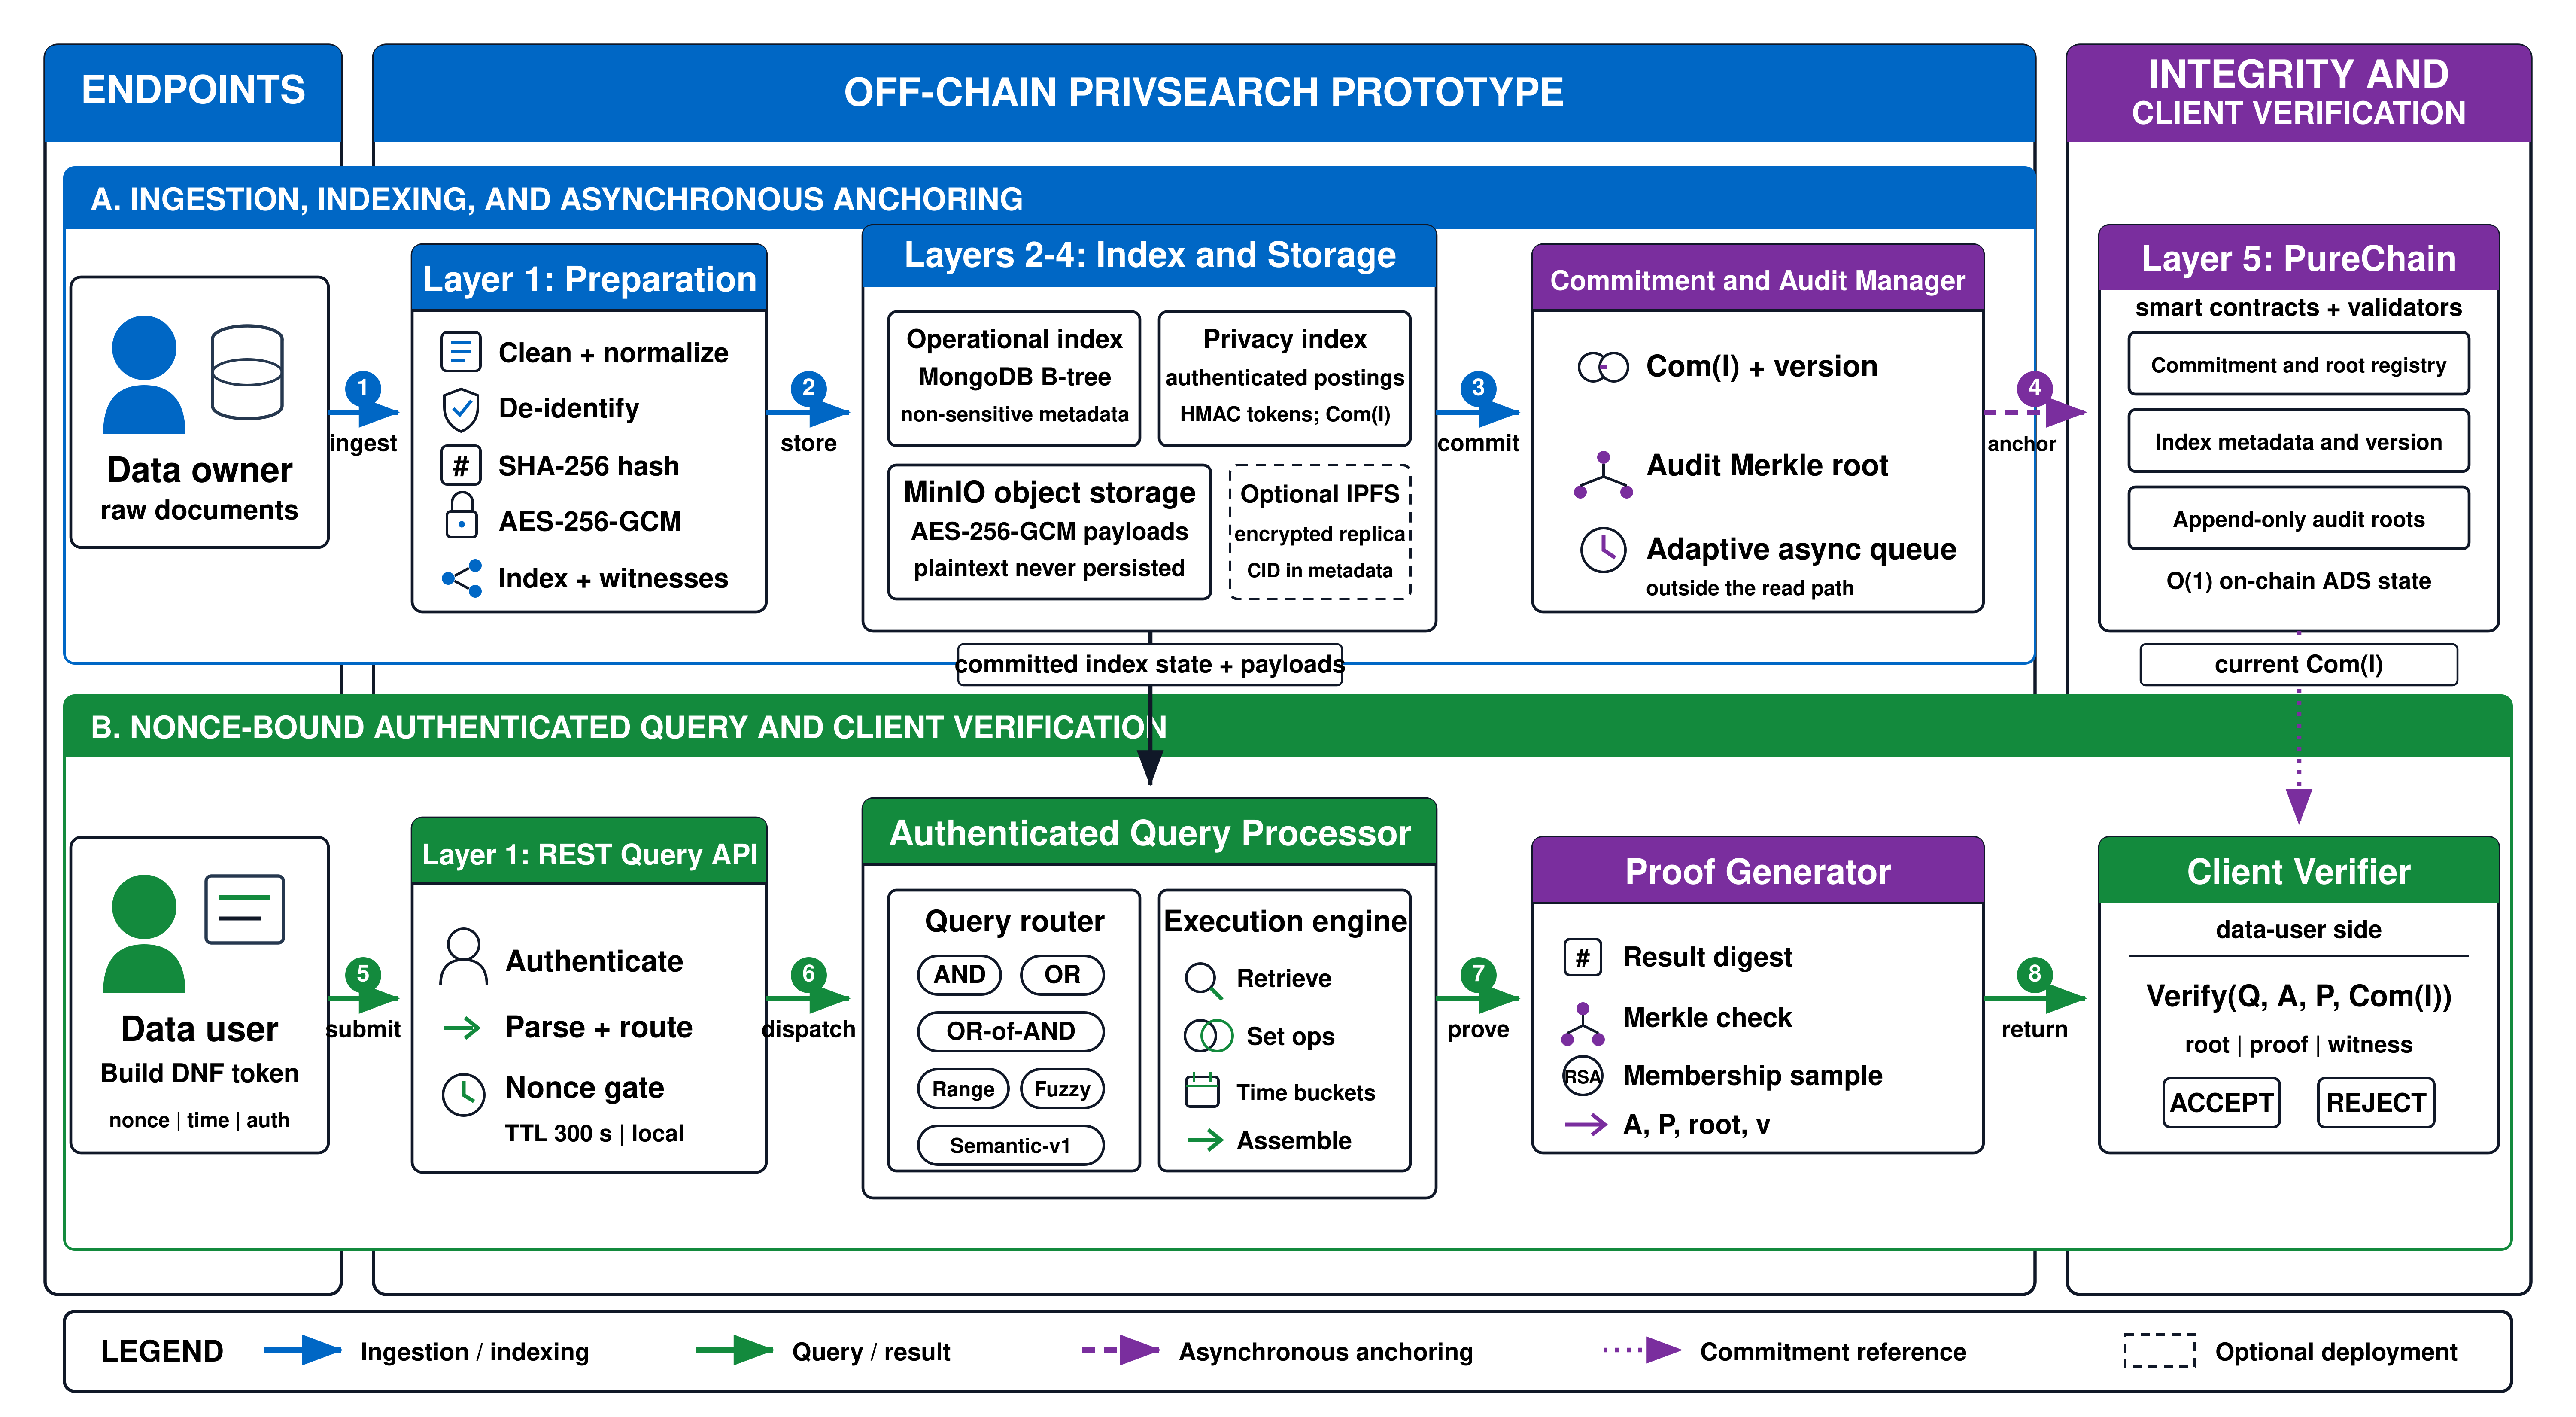
\includegraphics[width=0.80\textwidth]{pics/PrivSearch_System_Architecture.png}
\caption{PrivSearch architecture. Ingestion constructs authenticated encrypted indexes and asynchronously anchors their commitments on PureChain. Queries undergo nonce checking, authenticated search, proof generation, and client-side verification against the current commitment.}
\label{fig:architecture}
\end{figure*}

\textbf{Layer 1: Preparation and query API.}
During ingestion, the data owner cleans, normalizes, and de-identifies raw documents, computes their SHA-256 content hashes, encrypts payloads using AES-256-GCM, and constructs authenticated indexes and witnesses. During retrieval, the REST query API authenticates the data user, parses and routes the DNF query token, and applies a process-local nonce gate with validity window \(T\) (300~s in the prototype).

\textbf{Layers 2--4: Index and encrypted storage.}
Layer~2 maintains two complementary indexes. The operational index stores non-sensitive metadata in a MongoDB B-tree with lookup complexity \(O(\log n+|R|)\). The privacy index stores authenticated postings, HMAC-derived tokens, and the commitment \(\mathrm{Com}(I)\); its OXT-style conjunctive search cost depends on the least-frequent posting list, \(O(|R_{w_{\min}}|)\)~\cite{Yang}. Layer~3 stores AES-256-GCM-encrypted payloads in MinIO without persisting plaintext. Layer~4 optionally replicates encrypted objects through IPFS and records only their content identifiers in metadata.

\textbf{Authenticated query and proof processing.}
The query processor routes conjunctive, disjunctive, OR-of-AND, temporal-range, bounded-fuzzy, and semantic-v1 queries to the execution engine. The engine retrieves authenticated postings, performs the required set operations or time-bucket lookups, and assembles the answer. The proof generator returns the answer \(A\), proof \(P\), commitment root, and index version, including the result digest, Merkle evidence, and sampled RSA-accumulator witnesses.

\textbf{Off-chain commitment and audit manager.}
The manager constructs the versioned index commitment, computes Merkle roots over sealed audit batches, and places anchoring requests in an adaptive asynchronous queue. Its scheduler adjusts batch size according to \(\lambda/\mu\) without placing anchoring on the read-query critical path.

\textbf{Layer 5: PureChain integrity.}
PureChain smart contracts and validators maintain the commitment-and-root registry, index metadata and version, append-only audit roots, and the constant-size on-chain ADS state. The current \(\mathrm{Com}(I)\) is referenced by the data-user-side verifier, which evaluates
\[
\mathrm{Verify}(Q,A,P,\mathrm{Com}(I))
\]
and accepts or rejects the returned result.

\subsection{System Model and Notation}
\label{3B}

Let \(D=\{d_1,\ldots,d_n\}\) be the outsourced document set, \(W\) the keyword universe, \(I(w)\) the authenticated posting list for \(w\in W\), and \(M(d)\) the authenticated metadata of document \(d\). The current index commitment is denoted by \(\mathrm{Com}(I)\). For query \(Q\), answer \(A\), and proof \(P\), the client computes
\begin{equation}
\mathrm{Verify}(Q,A,P,\mathrm{Com}(I))
\in\{\mathrm{accept},\mathrm{reject}\}.
\end{equation}

After fuzzy or semantic expansion, every supported query is represented in disjunctive normal form:
\begin{equation}
Q=\bigvee_{i=1}^{d}C_i,\qquad
C_i=\bigwedge_j(k_j=v_j)\wedge
\bigwedge_l(r_l\in[a_l,b_l]),
\label{eq:dnf}
\end{equation}
and the final answer \(A=\bigcup_i\sigma_{C_i}(D)\) is deduplicated by document identifier.

We assume honest data owners and users, an append-only blockchain, and a potentially malicious off-chain server that may fabricate, alter, omit, or replay information~\cite{Yang,Yin,Wu}. Byzantine validators and validator collusion are outside the retrieval-layer threat model because consensus security belongs to the reused PureChain substrate.

\begin{table}[!tb]
\centering
\caption{Threat Model and Mitigation}
\label{tab:threat}
\scriptsize
\setlength{\tabcolsep}{3pt}
\begin{tabular}{p{1.25cm}p{1.35cm}p{1.55cm}p{1.9cm}}
\toprule
\textbf{Adversary} & \textbf{Goal} & \textbf{Capability} & \textbf{Mitigation} \\
\midrule
Malicious server &
Alter, omit, or fabricate results &
Controls storage and query execution &
Authenticated postings and committed index state; sampled soundness follows Theorem~\ref{thm:sampled} \\

Replay attacker &
Repeat an accepted mutation &
Replays valid request material &
Nonce-bound freshness and exact-match registry \\

Stale-proof attacker &
Return an outdated proof &
Reuses a prior valid transcript &
Equality check against current \(\mathrm{Com}(I)\) \\

Adaptive querier &
Infer sensitive structure &
Selects queries from prior outputs &
Encrypted postings and leakage-bounded trapdoors \\
\bottomrule
\end{tabular}
\end{table}

The analysis assumes DDH hardness for OXT cross-tags, pseudorandomness of HMAC-SHA256, authenticated-encryption security of AES-256-GCM under nonce uniqueness, and Strong RSA for the accumulator~\cite{CamenischLysyanskaya2002}. Experiments use a 2048-bit RSA modulus whose factorization was discarded after index preparation. One modular exponentiation costs \(175.2~\text{\textmu s}\) on Enron and \(174.0~\text{\textmu s}\) on the healthcare corpus. Production deployment requires either distributed modulus generation or a transparent accumulator, which remains outside the prototype scope. The prototype also integrates storage and query execution on the same stack; independent remote hosting remains future work.

\subsection{Authenticated Query Framework}
\label{3C}

PrivSearch supports six query families through authenticated posting-list intersection and union.

\subsubsection{Conjunctive Query}
\label{3C1}

For \(Q_{and}=w_1\wedge\cdots\wedge w_k\),
\begin{equation}
A_{and}=\bigcap_{j=1}^{k}I(w_j).
\label{eq:qand}
\end{equation}
This OXT-style path is also used for the same-stack SeaCQ comparison in Section~\ref{4G}.

\subsubsection{Disjunctive Query}
\label{3C2}

Each OR clause is evaluated and verified independently:
\begin{equation}
Q_{or}=\bigvee_{i=1}^{m}c_i,\qquad
A_{or}=\bigcup_{i=1}^{m}A(c_i),\quad
A(c_i)=\bigcap_{w\in c_i}I(w).
\label{eq:qor}
\end{equation}
The client rejects if any clause fails verification and otherwise returns the deduplicated union. Thus, OR support requires no additional trusted component.

\subsubsection{OR-of-AND Query}
\label{3C3}

General DNF queries are evaluated as
\begin{equation}
Q_{oa}=\bigvee_{i=1}^{p}
\left(\bigwedge_{j=1}^{q_i}w_{ij}\right),
\qquad
A_{oa}=\bigcup_{i=1}^{p}\bigcap_{j=1}^{q_i}I(w_{ij}).
\label{eq:qoa}
\end{equation}
Each conjunctive clause uses the AND engine, followed by verified deduplication.

\subsubsection{Temporal-Range Query}
\label{3C4}

Let \(\mathcal{B}(a,b)\) be the authenticated metadata buckets covered by \([a,b]\). Then
\begin{equation}
A_{range}=
\left(\bigcup_{t\in\mathcal{B}(a,b)}M^{-1}(t)\right)
\cap\bigcap_j I(k_j).
\label{eq:qrange}
\end{equation}
Each bucket is converted to a keyed token in the same namespace as keyword terms; literal bucket values are neither stored nor transmitted. A range query is therefore a union of \(B(a,b)=|\mathcal{B}(a,b)|\) authenticated lookups and requires no order-preserving encryption or its associated order leakage~\cite{Naveed2015}.

\subsubsection{Bounded Fuzzy Query}
\label{3C5}

For edit distance \(\operatorname{ed}(\cdot,\cdot)\), PrivSearch supports threshold-one matching:
\begin{equation}
Q_{\mathrm{fuzzy}}(w)=
\{w'\in W:\operatorname{ed}(w,w')\leq1\},
\qquad
A_{\mathrm{fuzzy}}=
\bigcup_{w'\in Q_{\mathrm{fuzzy}}(w)}I(w').
\label{eq:qfuzzy}
\end{equation}
This covers one insertion, deletion, or substitution, not arbitrary-distance similarity search.

\subsubsection{Semantic Query (v1)}
\label{3C6}

A concept \(c\) is mapped to a curated expansion set \(E(c)\) with client-known weights \(\omega_t\):
\begin{equation}
A_{sem}=\bigcup_{t\in E(c)}I(t),\qquad
\mathrm{score}(d)=
\sum_{\substack{t\in E(c)\\d\in I(t)}}\omega_t.
\label{eq:qsem}
\end{equation}
Results are ranked by \(\mathrm{score}(d)\) and verified against their authenticated postings. This executable semantic-v1 path performs concept expansion, not embedding-based retrieval.

\subsection{Replay-Protection Mechanism}
\label{3D}

Each state-mutating request carries
\((\mathit{nonce},\mathit{ts},\mathit{auth})\).
The bounded, TTL-evicting registry \(\mathcal{N}\) uses the key
\begin{equation}
\kappa=(\mathit{principal},\mathit{method},
\mathit{path},\mathit{nonce}),
\label{eq:noncekey}
\end{equation}
which binds freshness to a principal and endpoint. Admission is
\begin{equation}
\mathrm{Admit}(\kappa)=
\begin{cases}
\mathrm{reject}, & \kappa\in\mathcal{N},\\
\mathrm{insert}\ \kappa;\ \mathrm{process}, & \text{otherwise}.
\end{cases}
\label{eq:admit}
\end{equation}

The exact-match check precedes mutation and therefore rejects a repeated request while its key remains resident. This improves on the post-hoc replay detection of the reused substrate~\cite{Nnadiekwe2026PureSearchHCC}. The guarantee requires sufficient capacity \(C\) for all live keys within validity window \(T\). Moreover, the prototype registry is process-local and neither survives restart nor coordinates API replicas; horizontally scaled deployment requires a shared freshness store.

\subsection{Formal Security Analysis}
\label{3E}

\begin{definition}[Complete and sampled verifiers]
\label{def:completeverifier}
The complete verifier validates all authenticated membership and coverage evidence needed to reconstruct the committed answer. The sampled verifier checks membership witnesses for a uniformly selected subset of \(\min(s,|A|)\) returned documents. They coincide when \(|A|\leq s\). The prototype uses \(s=5\).
\end{definition}

\begin{theorem}[Conjunctive correctness]
\label{thm:conjcorrect}
Under the complete verifier, acceptance implies that every returned document satisfies all conjunctive terms in the committed index state.
\end{theorem}

\begin{proof}
Let \(d\in A_{and}\). By Eq.~\eqref{eq:qand}, \(d\) is returned only if it appears in every posting list \(I(w_j)\). The complete verifier authenticates each contributing posting against \(\mathrm{Com}(I)\). If \(d\notin I(w_j)\) for any \(j\), the corresponding membership evidence is invalid and verification rejects. Therefore, acceptance implies \(d\in\bigcap_{j=1}^{k}I(w_j)\), so every returned document satisfies all query terms.
\end{proof}

\begin{theorem}[Conjunctive completeness]
\label{thm:conjcomplete}
Under the complete verifier, acceptance implies that no valid committed conjunctive result is omitted.
\end{theorem}

\begin{proof}
Let
\[
R_{and}=\bigcap_{j=1}^{k}I(w_j)
\]
be the result induced by the committed postings. The complete verifier validates the authenticated coverage evidence for every contributing posting and reconstructs their deterministic intersection. If some \(d^{*}\in R_{and}\) were omitted from \(A_{and}\), then \(A_{and}\neq R_{and}\), causing the reconstructed result or its committed coverage digest to disagree with the submitted proof. The verifier would reject, contradicting acceptance. Hence \(A_{and}=R_{and}\).
\end{proof}

The preceding theorems apply to the complete verifier. They do not imply equivalent completeness for the prototype's sampled verifier.

\begin{theorem}[Sampled-verifier soundness]
\label{thm:sampled}
Let a returned set contain \(n\) documents, including \(t\geq1\) invalid documents. If \(s\leq n\) documents are sampled uniformly without replacement, then
\begin{equation}
p_{\det}(n,t,s)
=1-\frac{\binom{n-t}{s}}{\binom{n}{s}}
=1-\prod_{i=0}^{t-1}\frac{n-s-i}{n-i},
\label{eq:pdetect}
\end{equation}
with \(p_{\det}=1\) when \(s>n-t\). For \(t=1\),
\(p_{\det}=s/n\).
\end{theorem}

\begin{proof}
Detection fails exactly when all \(s\) checked documents are selected from the \(n-t\) valid documents. There are \(\binom{n-t}{s}\) such samples among \(\binom{n}{s}\) equiprobable samples. Therefore, the failure probability is their ratio and the detection probability is its complement. Expanding the ratio yields the product form. For \(t=1\), the failure probability reduces to \((n-s)/n\), giving \(p_{\det}=s/n\).
\end{proof}

\begin{corollary}[Required sampling rate]
\label{cor:floor}
Detecting one invalid document with probability at least \(1-\delta\) requires \(s\geq(1-\delta)n\). Hence, fixed-size sampling provides no result-size-independent detection floor.
\end{corollary}

\begin{proof}
For \(t=1\), Theorem~\ref{thm:sampled} gives \(p_{\det}=s/n\). Requiring \(s/n\geq1-\delta\) yields \(s\geq(1-\delta)n\). If \(s\) is fixed while \(n\) increases, then \(s/n\rightarrow0\).
\end{proof}

\begin{corollary}[Repeated interaction]
\label{cor:compound}
For \(q\) independent tampered responses with per-query detection probability \(p\), the probability of at least one detection is \(1-(1-p)^q\).
\end{corollary}

\begin{proof}
The probability that all \(q\) tampered responses avoid detection is \((1-p)^q\). Taking the complement gives the stated result.
\end{proof}

\begin{remark}[No omission completeness under sampling]
\label{rem:omission}
Because sampling selects only returned documents, an omitted document cannot be sampled. Therefore, the sampled verifier detects invalid inclusions probabilistically but does not establish completeness.
\end{remark}

Accordingly, zero verification failures under an honest server demonstrate functional correctness, not adversarial soundness. Tamper detection is evaluated separately in Section~\ref{4Ntd}.

\begin{theorem}[OR-query correctness and completeness]
\label{thm:orcorrect}
Let \(Q_{or}=c_1\lor\cdots\lor c_m\). If every clause answer is accepted under the complete verifier and the final answer is their deduplicated union, then the returned answer equals the committed OR-query result.
\end{theorem}

\begin{proof}
Let \(R(c_i)\) denote the committed result of clause \(c_i\). By Theorems~\ref{thm:conjcorrect} and~\ref{thm:conjcomplete}, acceptance of each clause gives \(A(c_i)=R(c_i)\). Therefore,
\[
A_{or}
=\bigcup_{i=1}^{m}A(c_i)
=\bigcup_{i=1}^{m}R(c_i).
\]
Deduplication removes only repeated identifiers and neither introduces an invalid document nor removes a distinct valid document. Hence \(A_{or}\) is exactly the committed OR-query result.
\end{proof}

\begin{corollary}[OR verification cost]
\label{cor:oradd}
OR verification cost is additive across independently authenticated clauses.
\end{corollary}

\begin{proof}
Each clause is evaluated and verified independently before union. The total verification work is therefore the sum of the clause-verification costs plus deduplication of their returned identifiers.
\end{proof}

\begin{theorem}[Range-query correctness and completeness]
\label{thm:rangecorrect}
Under the complete verifier, an accepted range answer equals the union of the committed buckets covered by \([a,b]\), intersected with any accompanying equality predicates.
\end{theorem}

\begin{proof}
Let
\[
R_{range}=
\left(\bigcup_{t\in\mathcal B(a,b)}M^{-1}(t)\right)
\cap\bigcap_j I(k_j).
\]
Every returned document must possess authenticated metadata placing it in a covered bucket and must satisfy each accompanying equality predicate. Thus, an out-of-range or predicate-violating document causes membership verification to fail. Conversely, the complete verifier authenticates the coverage of every bucket in \(\mathcal B(a,b)\) and the participating equality postings. Omitting a document from their deterministic union and intersection makes the submitted answer inconsistent with the authenticated coverage evidence. Therefore, acceptance implies \(A_{range}=R_{range}\).
\end{proof}

\begin{corollary}[Range-query cost]
\label{cor:rangecost}
Range-query cost increases with bucket count \(B(a,b)\) and candidate-set size \(|R_{range}|\).
\end{corollary}

\begin{proof}
The engine performs one authenticated lookup for each bucket in \(\mathcal B(a,b)\), followed by union, optional intersection, and verification over the resulting candidates. Hence work increases with both \(B(a,b)\) and \(|R_{range}|\).
\end{proof}

\begin{theorem}[Replay resistance under residency]
\label{thm:replay}
Assume that no live key is evicted from \(\mathcal{N}\) during freshness window \(T\). A request inducing key \(\kappa\) cannot cause two accepted state mutations within \(T\).
\end{theorem}

\begin{proof}
The first accepted request inserts \(\kappa\) before executing its mutation. Every subsequent request inducing the same key is checked against \(\mathcal N\) before mutation. Under the residency assumption, \(\kappa\) remains present and the exact-match lookup rejects the request. Therefore, the same freshness tuple cannot produce a second accepted mutation within \(T\).
\end{proof}

\begin{corollary}[Capacity condition]
\label{cor:evict}
For peak accepted-request rate \(\lambda\), residency is guaranteed when \(C\geq\lambda T\). If \(C<\lambda T\), admissible requests may evict a live key and invalidate the guarantee.
\end{corollary}

\begin{proof}
At most \(\lambda T\) distinct live keys arrive during a window of length \(T\). Capacity \(C\geq\lambda T\) therefore retains all live keys. If \(C<\lambda T\), an adversary that generates sufficiently many admissible keys can force eviction before expiry, after which the evicted request may be replayed.
\end{proof}

Replay checking has expected \(O(1)\) hash-table cost.

\begin{theorem}[Latency separation]
\label{thm:latsep}
Because the authenticated read path does not synchronously invoke anchoring, its protocol latency is independent of anchoring backlog, except for incidental contention over shared resources.
\end{theorem}

\begin{proof}
The query path comprises normalization, trapdoor generation, off-chain retrieval, proof generation, and client verification. Anchoring executes through a separate asynchronous queue and contributes no waiting term to this critical path. Increasing the anchoring backlog therefore does not change protocol-level read latency. Shared CPU, memory, disk, or network contention may affect observed latency, but such interference is an implementation effect rather than a protocol dependency.
\end{proof}

This restates Eq.~\eqref{eq:invariant} for encrypted retrieval; the underlying anchoring separation was established in~\cite{Nnadiekwe2026PureSearchHCC}.

\begin{definition}[PrivSearch leakage]
\label{def:leakage}
PrivSearch retains the OXT trapdoor, TSet, and cross-tag construction~\cite{Cash2013}. Its setup leakage is
\[
\mathcal{L}_{setup}(DB)=(|DB|,N),
\qquad
N=\sum_{w\in W}|I(w)|,
\]
and its query leakage is
\[
\mathcal{L}_{qry}(Q_t\mid Q_{<t})=
\bigl(
\mathrm{sp}(Q_t),
\mathrm{ap}(Q_t),
|R_{Q_t}|,
\mathrm{XP}(Q_t),
\mathrm{IP}(Q_t)
\bigr),
\]
where \(\mathrm{sp}\), \(\mathrm{ap}\), \(\mathrm{XP}\), and \(\mathrm{IP}\) denote the search, access, x-term equality, and conditional intersection patterns, respectively. Union-based queries additionally reveal their clause count.
\end{definition}

\begin{theorem}[Simulation-based query privacy]
\label{thm:sim}
Under DDH, secure pseudorandomness of \(F\), and secure authenticated encryption, PrivSearch is \(\mathcal{L}\)-secure in the random-oracle model:
\[
\left|
\Pr[\mathrm{Real}_{\Pi,\mathcal A}(\lambda)=1]
-\Pr[\mathrm{Ideal}_{\Pi,\mathcal A,\mathcal S}(\lambda)=1]
\right|
\leq\mathrm{negl}(\lambda).
\]
\end{theorem}

\begin{proof}[Proof sketch]
The conjunctive core retains the OXT trapdoor, TSet, and cross-tag constructions without modification. Under DDH and pseudorandomness of \(F\), the OXT simulator constructs an indistinguishable encrypted-index and query transcript using only \(\mathcal L_{setup}\) and \(\mathcal L_{qry}\). Secure authenticated encryption hides payload contents, while the accumulator can be simulated from the identifier set already exposed through the permitted access pattern. The union extension follows from Theorem~\ref{thm:union}. The complete real/ideal experiments and hybrid sequence are given in the supplementary material.
\end{proof}

\begin{theorem}[Union composition]
\label{thm:union}
If \(\Pi\) is \(\mathcal{L}\)-secure, independently evaluating \(m\) clauses and deduplicating their answers client-side is secure under
\[
\mathcal{L}'(\mathbf q)=
\bigl(m,\mathcal{L}(c_1),\ldots,\mathcal{L}(c_m)\bigr).
\]
\end{theorem}

\begin{proof}
Consider hybrids \(H_0,\ldots,H_m\), where \(H_j\) replaces the first \(j\) real clause transcripts with simulated transcripts. Adjacent hybrids differ in one invocation of \(\Pi\), so their distinguishing advantage is negligible by the \(\mathcal L\)-security of \(\Pi\). Summing over \(m\) hybrids gives at most \(m\cdot\mathrm{negl}(\lambda)\), which remains negligible for polynomial \(m\). Deduplication occurs client-side after decryption and therefore reveals no additional server-side overlap information. Hence the composed scheme is \(\mathcal L'\)-secure.
\end{proof}

\begin{remark}[Temporal-range coverage]
\label{rem:range}
A range query comprises \(B(a,b)\) independently trapdoored bucket lookups and is therefore covered by Theorem~\ref{thm:union}. Token shape does not distinguish bucket from equality lookups.
\end{remark}

The privacy result bounds leakage but does not eliminate access-pattern attacks, including query recovery~\cite{Islam2012,CashLeakage2015}, file injection~\cite{Zhang2016}, or volume-based range reconstruction~\cite{Grubbs2018}. The static prototype also provides neither forward nor backward privacy; dynamic schemes such as~\cite{Guo} remain complementary. The accumulator adds no information beyond the committed identifier set because its public witnesses can be simulated from that set.

\begin{theorem}[Cross-family security composition]
\label{thm:composition}
Let
\[
\mathcal Q=
\{Q_{\mathrm{and}},Q_{\mathrm{or}},Q_{\mathrm{oa}},
Q_{\mathrm{range}},Q_{\mathrm{fuzzy}},Q_{\mathrm{sem}}\}
\]
share commitment \(\mathrm{Com}(I)\) and nonce registry \(\mathcal N\). Under Strong RSA and the assumptions of Theorems~\ref{thm:replay} and~\ref{thm:sim}, the following properties hold without family-specific commitment material:

\begin{enumerate}[label=\textnormal{(\roman*)},topsep=2pt,itemsep=1pt]
\item accepted answers satisfy their authenticated query predicates; forging membership for an uncommitted identifier violates Strong RSA;

\item replay resistance applies uniformly to protected mutations, subject to nonce residency and the endpoint-bound key of Eq.~\eqref{eq:noncekey};

\item the complete verifier preserves correctness and completeness across families, whereas the sampled verifier provides only the guarantee of Theorem~\ref{thm:sampled}; and

\item adaptive multi-family transcripts remain simulatable under the leakage of Definition~\ref{def:leakage}, extended by clause counts according to Theorem~\ref{thm:union}.
\end{enumerate}
\end{theorem}

\begin{proof}[Proof sketch]
All query families reduce to authenticated intersections or unions of postings committed by the same \(\mathrm{Com}(I)\). Conjunctive correctness and completeness follow from Theorems~\ref{thm:conjcorrect} and~\ref{thm:conjcomplete}; OR, OR-of-AND, fuzzy, semantic-v1, and range queries preserve these properties through authenticated union by Theorems~\ref{thm:orcorrect}, \ref{thm:rangecorrect}, and~\ref{thm:union}. A forged membership witness for an uncommitted identifier contradicts Strong RSA. Replay resistance follows from the common pre-mutation registry check of Theorem~\ref{thm:replay}. Finally, Theorem~\ref{thm:sim} simulates the shared conjunctive core, while Theorem~\ref{thm:union} extends the simulation to union-based and range families. The sampled implementation inherits only Theorem~\ref{thm:sampled} and not complete omission detection. The full hybrid composition is provided in the supplementary material.
\end{proof}

Thus, one authenticated index commitment and one replay-protection channel serve all six query families.

\subsection{Analytical Cost Model}
\label{3F}

End-to-end query latency is decomposed as
\begin{equation}
\begin{aligned}
T_{query}(Q)={}&T_{norm}(Q)+T_{trapdoor}(Q)+T_{retrieve}(Q)\\
&+T_{proof}(Q)+T_{verify}(Q)+T_{anchor\_ref}(Q),
\end{aligned}
\label{eq:tquery}
\end{equation}
where \(T_{anchor\_ref}\) measures commitment-reference checking, not asynchronous anchoring.

For a \(k\)-term conjunctive query verifying sample \(R_s\),
\begin{equation}
T_{verify}(Q_{and})=
O(k+|R_s|t_{exp}).
\label{eq:tverify-and}
\end{equation}
For an \(m\)-clause OR query with deduplicated union \(U\),
\begin{equation}
T_{query}(Q_{or})=
\sum_{i=1}^{m}T_{query}(c_i)
+O\!\left(\sum_{i=1}^{m}|A(c_i)|\right),
\label{eq:tor}
\end{equation}
and
\begin{equation}
T_{verify}(Q_{or})=
\sum_{i=1}^{m}T_{verify}(c_i)+O(|U|).
\label{eq:tverify-or}
\end{equation}
For a temporal range,
\begin{equation}
T_{query}(Q_{range})=
O\!\left(B(a,b)+|R_{range}|+|R_s|t_{exp}\right).
\label{eq:trange}
\end{equation}

Let \(S_{index}=S_{enc}+S_{meta}\). Storage overhead is
\begin{equation}
\rho_{storage}=\frac{S_{index}}{S_{raw}},
\label{eq:rho}
\end{equation}
and proof size is
\begin{equation}
S_{proof}=O(kb_{root}+|R_s|b_{wit}).
\label{eq:sproof}
\end{equation}

\begin{table}[!tb]
\centering
\caption{PrivSearch Complexity}
\label{tab:complexity}
\scriptsize
\setlength{\tabcolsep}{3pt}
\begin{tabular}{p{2.5cm}p{2.3cm}p{1.8cm}}
\toprule
\textbf{Operation} & \textbf{Complexity} & \textbf{Driver} \\
\midrule
Metadata search &
\(O(\log n+|R|)\) &
Result size \\

Conjunctive search &
\(O(|R_{w_{\min}}|)\) &
Smallest posting \\

Disjunctive search &
\(O(\sum_i|R_{w_{\min}}^{(i)}|)\) &
Clause postings \\

Range search &
\(O(B+|R_{range}|)\) &
Buckets and results \\

Complete verification &
\(O(|R|kt_{exp})\) &
All witnesses \\

Sampled verification &
\(O(\min(s,|R|)kt_{exp})\) &
Sample size \\

Returned-set digest &
\(O(|R|t_h)\) &
All returned records \\

Witness precomputation &
\(O(\sum_w|I(w)|^2t_{exp})\) &
Posting-list sizes \\

Merkle batching &
\(O(b)\) &
Batch size \\

Blockchain anchor &
\(O(1)\) &
Fixed root \\

Replay lookup &
Expected \(O(1)\) &
Exact-match hash \\

On-chain ADS &
\(O(1)\) &
Accumulator value \\
\bottomrule
\end{tabular}
\end{table}

At fixed \(s\), sampled witness checking is constant in \(|R|\), but returned-set hashing remains linear. Sampling therefore reduces accumulator work without establishing omission completeness or eliminating result-size-dependent verification cost. 
 
% \section{System Methodology}
% \label{3}
% This section presents the PrivSearch architecture, system and adversary model, unified authenticated query framework, replay-protection mechanism, formal security analysis, and the cost model linking those properties to the timings measured in Section~\ref{4}. The analysis culminates in a composition theorem (Theorem~\ref{thm:composition}) stating why PrivSearch's guarantee is a new claim rather than a consequence of prior single-family results.

% \subsection{Design Principles and System Architecture}
% \label{3A}
% PrivSearch is built around one architectural invariant: operational query latency must remain decoupled from blockchain anchoring latency. Writing $T_{search}$ for operational and encrypted search latency and $T_{anchor}$ for asynchronous anchoring latency, we require
% \begin{equation}
% T_{search} \perp T_{anchor},
% \label{eq:invariant}
% \end{equation}
% so that read-query latency is architecturally independent of the anchoring backlog. This invariant and the anchoring plane realizing it were established for plaintext indexed metadata in~\cite{Nnadiekwe2026PureSearchHCC} and are reused rather than newly claimed; the present contribution is the authenticated encrypted retrieval layer above it, realized by the five-layer architecture of Fig.~\ref{fig:architecture}.

% \begin{figure*}[!t]
% \centering
% 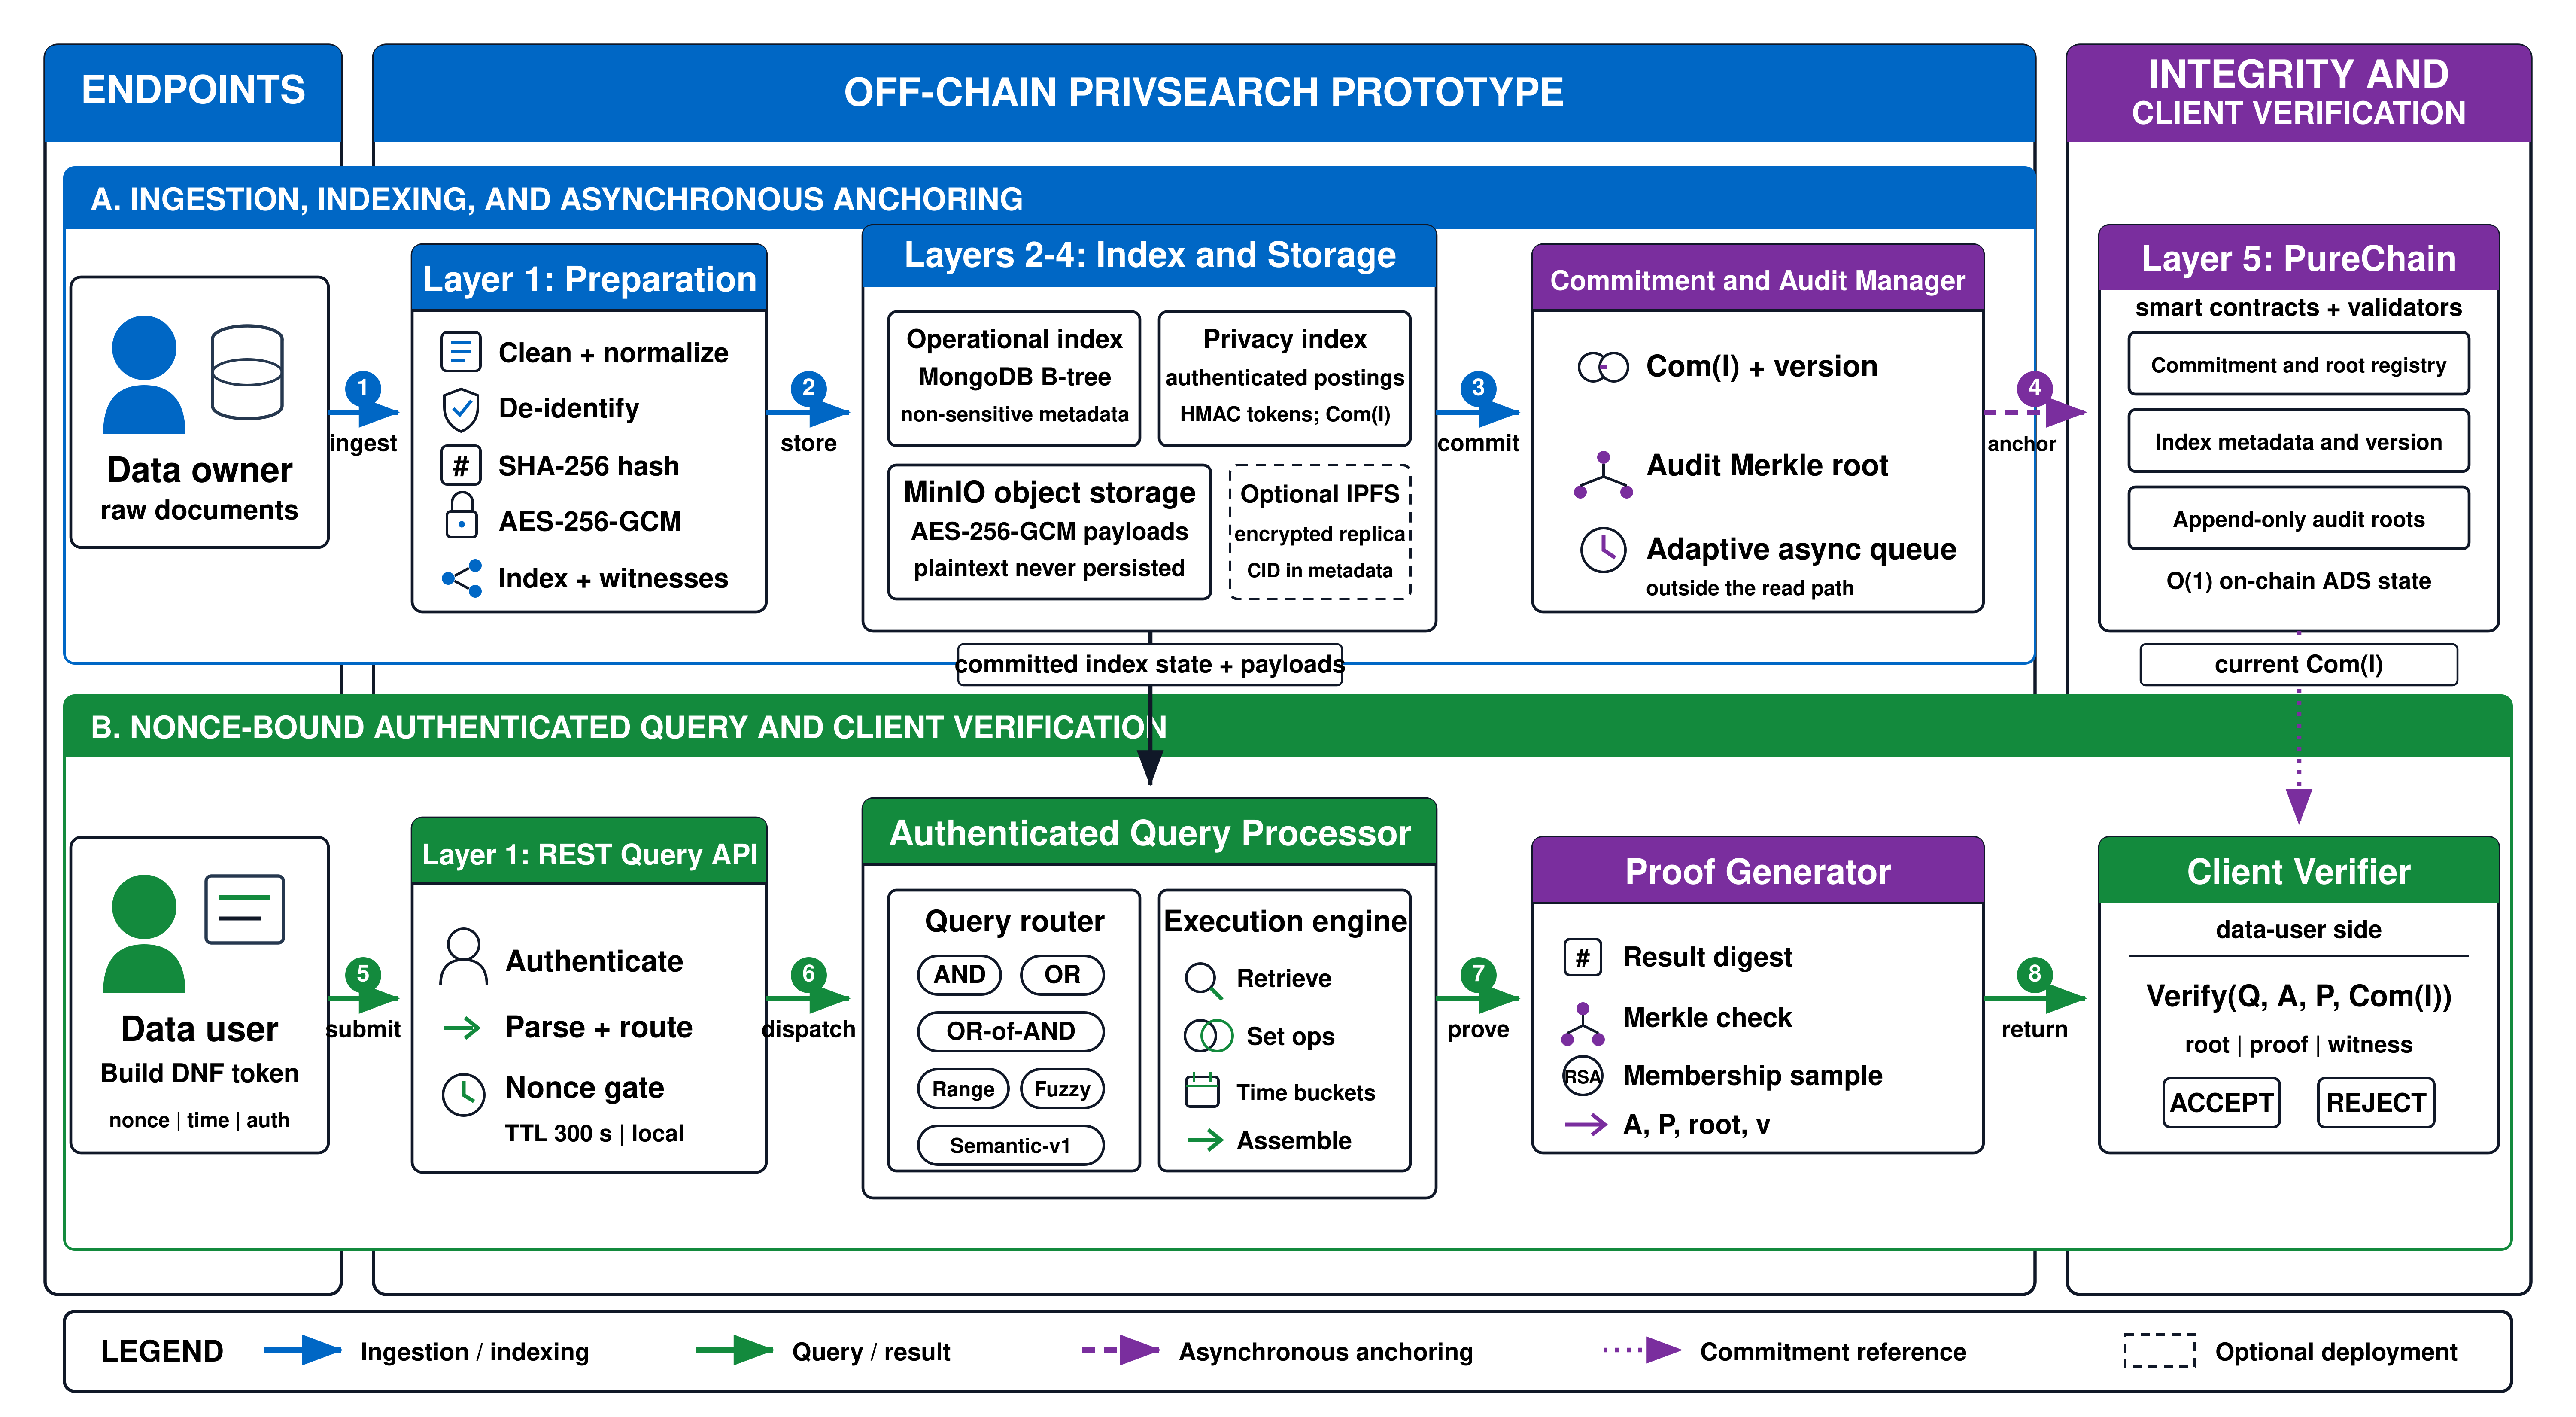
\includegraphics[width=0.80\textwidth]{pics/PrivSearch_System_Architecture.png}
% \caption{PrivSearch system architecture. The ingestion path constructs and
% stores authenticated encrypted indexes before asynchronously anchoring their
% commitments on PureChain. The query path performs nonce checking, authenticated search and proof generation, followed by client-side verification against the current on-chain commitment.}
% \label{fig:architecture}
% \end{figure*}

% \textbf{Layer 1 (Application)} exposes a REST interface for ingestion, query submission, and administration, and attaches a freshness tuple to every state-mutating request.

% \textbf{Layer 2 (Dual-layer index)} is the core architectural contribution. An \emph{operational index} holds non-sensitive attributes in plaintext B-trees for administrative lookups ($O(\log n + |R|)$); a \emph{privacy index} holds an authenticated encrypted index over sensitive keyword and metadata attributes, extending the OXT protocol used by SeaCQ~\cite{Yang}, which attains conjunctive complexity $O(|R_{w_{min}}|)$ by intersecting candidates around the least-frequent keyword. Both paths satisfy Eq.~\eqref{eq:invariant} independently of anchor-queue state.

% \textbf{Layer 3 (Encrypted object storage)} stores AES-256-GCM payloads with a SHA-256 content hash computed before encryption; plaintext is never persisted. \textbf{Layer 4 (Decentralized replication, optional)} distributes encrypted replicas across content-addressed storage for cross-institution access, recording only the content identifier in metadata.

% \textbf{Layer 5 (Blockchain integrity)} anchors three mechanisms on PureChain: (i) an RSA-accumulator authenticated data structure (ADS) giving per-query correctness and completeness proofs at $O(1)$ on-chain storage rather than $O(s_r+s_c)$, following the constant-size construction of SeaCQ$^{*}$; (ii) Merkle batch anchoring, hashing sealed batches of audit transactions into a root anchored asynchronously at $O(1)$ amortized gas per batch; and (iii) the bounded, TTL-evicting nonce registry of Section~\ref{3D}, performing exact-match replay detection at the API boundary. An adaptive scheduler monitors the arrival-to-processing ratio $\lambda/\mu$ and adjusts batch size $b$ so backlog growth stays bounded without ever blocking the query path, operationally realizing Eq.~\eqref{eq:invariant} under bursty write load.

% \subsection{System Model and Notation}
% \label{3B}
% Let $D=\{d_1,\dots,d_n\}$ denote the outsourced document set and $W$ the keyword universe. Let $I(w)$ denote the authenticated posting list for keyword $w \in W$, $M(d)$ the authenticated metadata bound to document $d$ (e.g., month/year buckets used for range queries), and $\mathrm{Com}(I)$ the authenticated commitment of the current index state, anchored on-chain. For a query $Q$ the server returns an answer set $A$ and proof object $P$; the client-side verifier computes
% \begin{equation}
% \mathrm{Verify}(Q,A,P,\mathrm{Com}(I)) \in \{\text{accept}, \text{reject}\}.
% \end{equation}
% We consider conjunctive $Q_{and}$, disjunctive $Q_{or}$, range $Q_{range}$, and fuzzy $Q_{fuzzy}$ classes, together with the concept-expanded semantic query $Q_{sem}$ of Section~\ref{3C6}. Every PrivSearch query is expressible in disjunctive normal form,
% \begin{equation}
% Q = C_1 \lor C_2 \lor \cdots \lor C_d, \quad
% C_i = \bigwedge_{j} (k_j = v_j) \wedge \bigwedge_{l} \big(r_l \in [a_l,b_l]\big),
% \label{eq:dnf}
% \end{equation}
% where each clause $C_i$ conjoins equality predicates over searchable keyword attributes $k_j$ with optional range predicates over attributes $r_l$, and the final answer $A = \bigcup_i \sigma_{C_i}(D)$ is deduplicated on document identifier.

% The trust and adversary model follows the semi-honest/malicious cloud model of prior authenticated blockchain query work~\cite{Yang,Yin,Wu}: the data owner and data user are honest, the blockchain platform is honest and append-only, and the off-chain cloud server (storage and query execution) is potentially malicious, in that it may return incorrect, incomplete, stale, or fabricated results, or replay previously accepted requests. Table~\ref{tab:threat} summarizes the four adversaries against which PrivSearch states a guarantee. Byzantine and colluding \emph{validators} are deliberately excluded: threshold validation is a property of the underlying PureChain substrate rather than of the retrieval layer contributed here, and the benchmark of Section~\ref{4O} measures its latency under network delay, not its resistance to a Byzantine quorum. We therefore make no adversarial claim about validator behavior.

% Section~\ref{3E} assumes DDH hardness in the group underlying the OXT cross-tag construction, pseudorandomness of the keyed function $F$ (HMAC-SHA256), IND-CPA security of AES-256-GCM, and Strong RSA for the membership accumulator~\cite{CamenischLysyanskaya2002}, which further presumes an RSA modulus whose factorization is unknown to all parties. All results in Section~\ref{4} use a 2048-bit modulus generated once during index preparation with the factorization discarded; one modular exponentiation costs a measured $t_{exp}=175.2$~\textmu s (Enron) and $174.0$~\textmu s (healthcare), and every verification figure in this paper is a multiple of that cost rather than of a reduced-parameter proxy. Production deployment would require a distributed generation ceremony or a class-group instantiation needing no trusted setup, which we state as an open requirement rather than a solved problem.

% \begin{table}[!tb]
% \centering
% \caption{Threat Model and Mitigation}
% \label{tab:threat}
% \scriptsize
% \setlength{\tabcolsep}{3pt}
% \begin{tabular}{p{1.3cm}p{1.4cm}p{1.55cm}p{1.85cm}}
% \toprule
% \textbf{Adversary} & \textbf{Goal} & \textbf{Capability} & \textbf{Mitigation} \\
% \midrule
% Malicious cloud server & Alter, omit, or fabricate results & Controls outsourced storage/query execution & Authenticated postings, proof verification, committed index state (Theorem~\ref{thm:sampled} bounds the sampled case) \\
% Replay attacker & Resubmit accepted writes & Captures/replays valid request material & Nonce-bound freshness checks, exact-match nonce registry (Theorem~\ref{thm:replay}) \\
% Stale-proof attacker & Return once-valid, outdated proofs & Reuses proof from earlier state & Root-equality check against current $\mathrm{Com}(I)$ (Section~\ref{4N}) \\
% Adaptive query adversary & Infer sensitive structure & Chooses queries adaptively from outputs & Encrypted postings, trapdoor interface; leakage bounded by Definition~\ref{def:leakage} \\
% \bottomrule
% \end{tabular}
% \end{table}

% PrivSearch is evaluated under this model using a runnable prototype integrated with the hybrid blockchain stack rather than a physically separate, independently hosted cloud server; a remote query-server benchmark remains future work.

% \subsection{Authenticated Query Framework}
% \label{3C}
% PrivSearch supports six query families under the unified DNF model of Eq.~\eqref{eq:dnf}.

% \subsubsection{Conjunctive Baseline}
% \label{3C1}
% The conjunctive query $Q_{and}=w_1 \wedge \cdots \wedge w_k$ follows the OXT-style AND-search model used by SeaCQ: a record is returned only if it belongs to every contributing authenticated posting list $I(w_1),\dots,I(w_k)$. This family is the direct experimental baseline against SeaCQ (Section~\ref{4G}).

% \subsubsection{Disjunctive OR Query}
% \label{3C2}
% A disjunctive query is evaluated clause-by-clause and recombined from authenticated clause-level results:
% \begin{equation}
% \begin{aligned}
% Q_{\mathrm{or}}
%     &= c_1 \lor c_2 \lor \cdots \lor c_m,\\
% A_{\mathrm{or}}
%     &= \bigcup_{i=1}^{m} A(c_i),
%     \qquad
% A(c_i)=\bigcap_{w\in c_i} I(w).
% \end{aligned}
% \label{eq:qor}
% \end{equation}
% Each clause \(c_i\) is evaluated by the conjunctive engine and authenticated against its posting lists, and \(A_{\mathrm{or}}\) is the deduplicated union of clause answers that pass verification, so the client authenticates the OR result without an additional trusted component rather than concatenating unauthenticated outputs (Algorithm~\ref{alg:authenticated-or}).

% \begin{algorithm}[t]
% \caption{Authenticated OR-Query Evaluation}
% \label{alg:authenticated-or}
% \begin{algorithmic}[1]
% \Require Query $Q_{\mathrm{or}}=c_1\lor\cdots\lor c_m$,
% commitment $\mathrm{Com}(I)$
% \Ensure Verified answer $A_{\mathrm{or}}$ and proof $P_{\mathrm{or}}$

% \State $A_{\mathrm{or}}\gets\emptyset$
% \State $P_{\mathrm{or}}\gets\emptyset$

% \For{$i=1$ to $m$}
%     \State $(A(c_i),P(c_i))
%     \gets \Call{EvaluateClause}{c_i}$

%     \If{$\mathrm{Verify}\bigl(c_i,A(c_i),P(c_i),
%         \mathrm{Com}(I)\bigr)=\mathit{reject}$}
%         \State \textbf{abort}
%         \Comment{Clause verification failed}
%     \EndIf

%     \State $A_{\mathrm{or}}\gets
%     A_{\mathrm{or}}\cup A(c_i)$
%     \Comment{Deduplicate by document ID}

%     \State $P_{\mathrm{or}}\gets
%     P_{\mathrm{or}}\cup P(c_i)$
% \EndFor

% \State \Return $(A_{\mathrm{or}},P_{\mathrm{or}})$
% \end{algorithmic}
% \end{algorithm}

% \subsubsection{OR-of-AND Query}
% \label{3C3}
% PrivSearch further supports small-clause-count disjunctive normal form,
% \begin{equation}
% Q_{oa} = \bigvee_{i=1}^{p}\Big(\bigwedge_{j=1}^{q_i} w_{ij}\Big), \qquad
% A_{oa} = \bigcup_{i=1}^{p}\ \bigcap_{j=1}^{q_i} I(w_{ij}),
% \label{eq:qoa}
% \end{equation}
% e.g., $(w_1 \wedge w_2) \lor (w_3 \wedge w_4)$, capturing realistic ``alternative constrained case'' queries rather than single-keyword alternation alone. Each conjunctive clause is evaluated by the standard AND engine and the verified clause outputs are combined by the deduplicated-union procedure of Algorithm~\ref{alg:authenticated-or}.

% \subsubsection{Temporal Range Query}
% \label{3C4}
% Range queries are evaluated over authenticated metadata buckets $M(d)$ keyed by month or year. Let $\mathcal{B}(a,b) = \{\, t : t \text{ is a metadata bucket}, a \le t \le b \,\}$ be the buckets covered by $[a,b]$ and $B(a,b)=|\mathcal{B}(a,b)|$ their number. The engine computes
% \begin{equation}
% A_{range} = \Big(\bigcup_{t \in \mathcal{B}(a,b)} M^{-1}(t)\Big) \cap \bigcap_{j} I(k_j),
% \label{eq:qrange}
% \end{equation}
% where $M^{-1}(t)=\{d \in D : t \in M(d)\}$, and the optional intersection with $I(k_j)$ applies any accompanying equality predicates as in Eq.~\eqref{eq:dnf}: PrivSearch resolves $[a,b]$ to $\mathcal{B}(a,b)$, retrieves and authenticates postings per bucket, then unions and verifies the candidate set.

% Crucially, the range path uses no order-preserving encryption. Each bucket $t$ is resolved to a posting token \texttt{meta:}$\langle$field$\rangle$\texttt{:}$\langle$value$\rangle$ passed through the \emph{same} keyed trapdoor derivation and token namespace as ordinary keyword terms before any index lookup; the literal bucket string is never stored or transmitted. A range query is therefore structurally a disjunction of $B(a,b)$ independently trapdoored posting-list lookups indistinguishable by token shape from equality lookups. Two consequences follow: the family inherits the union-composition guarantee of Theorem~\ref{thm:union} (Remark~\ref{rem:range}), and no order leakage of the kind exploited against property-preserving encryption~\cite{Naveed2015} arises.

% \subsubsection{Bounded Fuzzy Matching}
% \label{3C5}
% With $ed(w,w')$ the edit (Levenshtein) distance between $w,w' \in W$, PrivSearch supports bounded fuzzy matching at threshold one,
% \begin{equation}
% \begin{aligned}
% Q_{\mathrm{fuzzy}}(w)
%     &= \{\,w' \in W : \operatorname{ed}(w,w') \leq 1\,\},\\
% A_{\mathrm{fuzzy}}
%     &= \bigcup_{w' \in Q_{\mathrm{fuzzy}}(w)} I(w'),
% \end{aligned}
% \label{eq:qfuzzy}
% \end{equation}
% so that $w$ retrieves the authenticated union of postings for every keyword within one insertion, deletion, or substitution. This is intentionally a bounded model rather than similarity search over arbitrary edit distance.

% \subsubsection{Semantic Query (v1)}
% \label{3C6}
% The semantic path (\emph{semantic\_v1}) represents a high-level concept $c$ as a curated expansion-term set $E(c)=\{t_1,\dots,t_r\} \subseteq W$ with per-term weights $\omega_1,\dots,\omega_r$, computing
% \begin{equation}
% A_{sem} = \bigcup_{t \in E(c)} I(t), \qquad
% \mathrm{score}(d) = \!\!\sum_{t \in E(c)\,:\,d \in I(t)}\!\! \omega_t,
% \label{eq:qsem}
% \end{equation}
% ranking by $\mathrm{score}(d)$ and verifying the ranked output against the underlying authenticated postings. Grounding expansion in authenticated postings rather than a neural embedding index keeps verification tractable; this is a first-generation executable semantic path, not an embedding-based retrieval system.

% \subsection{Replay-Protection Mechanism}
% \label{3D}
% Every state-mutating request carries a freshness tuple $(\mathit{nonce}, \mathit{ts}, \mathit{auth})$. The \emph{nonce registry} $\mathcal{N}$ is a bounded in-memory key--value store with time-to-live eviction, keyed on
% \begin{equation}
% \kappa = \bigl(\mathit{principal},\, \mathit{method},\, \mathit{path},\, \mathit{nonce}\bigr),
% \label{eq:noncekey}
% \end{equation}
% binding freshness to a specific principal invoking a specific endpoint rather than to a principal-global counter. Entries expire after a configurable validity window $T$ (e.g., 24 hours for clinical event deduplication), and the store enforces a capacity bound $C$ by evicting the oldest surviving entry when full. Admission is
% \begin{equation}
% \mathrm{Admit}(\kappa)=
% \begin{cases}
% \text{reject (\texttt{DUPLICATE\_EVENT})}, & \kappa \in \mathcal{N},\\[2pt]
% \text{insert } \kappa;\ \text{process}(\mathit{event}), & \text{otherwise.}
% \end{cases}
% \label{eq:admit}
% \end{equation}

% Lookup is exact-match, so admission has neither false positives nor false negatives within the validity window: no fresh request is rejected as a duplicate, and no duplicate is admitted while its key remains resident. The check executes \emph{before} any state mutation, so a replayed request cannot cause a second accepted write. This targets a gap in the prior hybrid-blockchain evidence underlying this work~\cite{Nnadiekwe2026PureSearchHCC}, where replay attempts were detectable only after the fact through audit inspection rather than rejected in real time; Section~\ref{4N} reports the live benchmark.

% Two deployment boundaries follow and are stated explicitly. First, residency holds only while $C$ exceeds the number of distinct admissible keys arriving within $T$; Corollary~\ref{cor:evict} gives the consequences of violating that bound. Second, the registry is process-local, so it neither survives a restart nor is shared across horizontally scaled API replicas; a multi-replica deployment requires a shared freshness store, outside the present prototype scope.

% \subsection{Formal Security Analysis}
% \label{3E}
% We state the correctness, completeness, replay-resistance, latency-separation, and query-privacy properties of PrivSearch as definition--theorem--proof triples, connecting each to its experimental evidence in Section~\ref{4}. We first fix the verifier to which the correctness and completeness results apply.

% \begin{definition}[Complete and sampled verifiers]
% \label{def:completeverifier}
% The \emph{complete verifier} checks an authenticated membership witness for every document in the returned answer set $A$. The \emph{sampled verifier} with parameter $s$ checks witnesses for a uniformly random subset of $\min(s,|A|)$ documents of $A$; for $|A| \le s$ the two coincide. Theorems~\ref{thm:conjcorrect}, \ref{thm:conjcomplete}, \ref{thm:orcorrect} and~\ref{thm:rangecorrect} are stated for the complete verifier. The deployed prototype uses the sampled verifier with default $s=5$, whose guarantee is Theorem~\ref{thm:sampled}.
% \end{definition}

% Throughout, $Q_{and}=w_1 \wedge \cdots \wedge w_k$ has committed authenticated posting lists $I(w_1),\dots,I(w_k)$, and $\mathrm{Verify}$ accepts only if $(A,P)$ is consistent with $\mathrm{Com}(I)$.

% \begin{theorem}[Conjunctive correctness]
% \label{thm:conjcorrect}
% Under the complete verifier of Definition~\ref{def:completeverifier}, if $\mathrm{Verify}(Q_{and},A_{and},P_{and})$ accepts, then every document in $A_{and}$ satisfies all conjunctive query terms under the committed dataset state.
% \end{theorem}
% \begin{proof}[Proof sketch]
% Acceptance implies every posting list used is authenticated against $\mathrm{Com}(I)$, and $A_{and}$ is computed only from $I(w_1)\cap\cdots\cap I(w_k)$; a document violating any term fails membership consistency with at least one authenticated list and causes rejection. Full proof in the supplementary material.
% \end{proof}

% \begin{theorem}[Conjunctive completeness]
% \label{thm:conjcomplete}
% Under the complete verifier, if $\mathrm{Verify}(Q_{and},A_{and},P_{and})$ accepts, then no valid committed conjunctive result is omitted from $A_{and}$.
% \end{theorem}
% \begin{proof}[Proof sketch]
% An omitted $d^{*}$ from the true committed intersection would make the answer inconsistent with the deterministic intersection induced by the committed state, so the verifier rejects, contradicting acceptance. Full proof in the supplementary material.
% \end{proof}

% The deployed prototype uses the sampled verifier, so its guarantee is probabilistic. This matters for the zero verification failures of Sections~\ref{4D} and~\ref{4F}: those runs exercise an honest server and evidence that the verifier accepts correct answers, not soundness against a tampering server, which Section~\ref{4Ntd} measures separately.

% \begin{theorem}[Soundness of the sampled verifier]
% \label{thm:sampled}
% Let $|A| = n$ be the size of a returned answer set of which $t \ge 1$ documents are not members of the committed result, and let the verifier check a uniformly random sample of size $s \le n$. The probability that at least one tampered document is checked is
% \begin{equation}
% p_{\det}(n,t,s) \;=\; 1 - \frac{\binom{n-t}{s}}{\binom{n}{s}}
% \;=\; 1 - \prod_{i=0}^{t-1}\frac{n-s-i}{n-i},
% \label{eq:pdetect}
% \end{equation}
% with $p_{\det}=1$ whenever $s > n-t$. In particular, for a single tampered document, $p_{\det}(n,1,s) = s/n$.
% \end{theorem}
% \begin{proof}
% Detection fails exactly when the sample avoids all $t$ tampered documents. The number of $s$-subsets drawn from the $n-t$ untampered documents is $\binom{n-t}{s}$, out of $\binom{n}{s}$ equiprobable samples; the product form follows by expanding the binomial ratio. For $t=1$ the ratio reduces to $(n-s)/n$.
% \end{proof}

% \begin{corollary}[Sampling cost of a detection floor]
% \label{cor:floor}
% To achieve $p_{\det}\ge 1-\delta$ against a single tampered document, Theorem~\ref{thm:sampled} requires $s \ge (1-\delta)n$. A constant detection floor therefore costs a constant \emph{fraction} of the answer set, and no sublinear sampling rule attains a detection floor independent of $n$ against $t=1$. Holding $s$ fixed while $n$ grows drives $p_{\det}\to 0$.
% \end{corollary}

% \begin{corollary}[Detection under repeated interaction]
% \label{cor:compound}
% A server that tampers across $q$ independent queries, each with per-query detection probability $p$, is detected at least once with probability $1-(1-p)^{q}$. Sampled verification therefore provides auditing-grade detection against a persistently tampering server rather than per-query soundness against a single-shot adversary.
% \end{corollary}

% \begin{remark}[Omission is not covered by sampling]
% \label{rem:omission}
% Sampling draws from the \emph{returned} answer set, so a document omitted from $A$ can never be selected. The sampled verifier therefore provides no completeness guarantee at any $s<n$; completeness requires the complete verifier of Definition~\ref{def:completeverifier}.
% \end{remark}

% \begin{theorem}[OR-query correctness]
% \label{thm:orcorrect}
% Let $Q_{or}=c_1\lor\cdots\lor c_m$ with each clause $c_i$ individually authenticated. Under the complete verifier, if every clause answer $A(c_i)$ is accepted and the final answer is the deduplicated union of accepted clause answers, then the returned OR answer equals the committed OR-query result.
% \end{theorem}
% \begin{proof}[Proof sketch]
% Clause-level acceptance gives $A(c_i)=R(c_i)$ for every $i$; deduplication removes only repeated identifiers, and no document failing all clauses appears in an accepted clause answer. Hence $A_{or}$ equals the committed union.
% \end{proof}

% \begin{corollary}[Additive OR verification cost]
% \label{cor:oradd}
% Authenticated OR execution introduces additive clause-wise proof handling and verification cost across independently verified clauses, as the OR benchmarks of Section~\ref{4D} confirm.
% \end{corollary}

% \begin{theorem}[Range-query correctness]
% \label{thm:rangecorrect}
% Let $Q_{range}=[a,b]$ be a metadata-backed interval query over authenticated month or year buckets derived from the committed dataset state. Under the complete verifier, if $\mathrm{Verify}(Q_{range},A_{range},P_{range})$ accepts, then $A_{range}$ is exactly the committed range-query result set for $[a,b]$.
% \end{theorem}
% \begin{proof}[Proof sketch]
% Accepted records are consistent with authenticated metadata bindings and lie within $[a,b]$; omission would break consistency with the committed coverage and cause rejection. Acceptance therefore implies neither false positives nor false negatives.
% \end{proof}

% \begin{corollary}[Range-cost dependence]
% \label{cor:rangecost}
% The cost of authenticated range retrieval increases with interval breadth $B(a,b)$ and candidate-set size $|R_{range}|$, as the month- and year-range benchmarks of Section~\ref{4D} confirm.
% \end{corollary}

% \begin{theorem}[Replay resistance under residency]
% \label{thm:replay}
% Let a state-mutating request carry freshness material $(\mathit{nonce},\mathit{ts})$ inducing the registry key $\kappa$ of Eq.~\eqref{eq:noncekey}, accepted only if $\kappa$ is not resident in $\mathcal{N}$ at the time of the check. Let $T$ denote the freshness window and $C$ the registry capacity, and suppose no eviction of a live key occurs during $T$. Then a replay attacker cannot obtain two accepted mutations from the same freshness tuple within $T$.
% \end{theorem}
% \begin{proof}
% After the first valid request is accepted, $\kappa$ is inserted into $\mathcal{N}$ before the mutation executes. Any subsequent request inducing the same $\kappa$ is tested against $\mathcal{N}$ before mutation. Under the residency hypothesis $\kappa$ is still present, the lookup is exact, and the request is rejected. Hence no second accepted mutation arises from the same freshness tuple within $T$.
% \end{proof}

% \begin{corollary}[Capacity condition for residency]
% \label{cor:evict}
% Let $\lambda$ denote the peak rate of accepted state-mutating requests bearing distinct keys. Residency holds, and hence Theorem~\ref{thm:replay} applies, whenever $C \ge \lambda T$. If $C < \lambda T$, an adversary able to issue $C$ distinct admissible requests within $T$ can evict a target key before its expiry and subsequently replay it. Registry sizing is therefore a security parameter rather than a performance parameter.
% \end{corollary}

% Under exact-match hash-table lookup, replay checking has expected $O(1)$ overhead beyond ordinary implementation cost; we refer to this as the $O(1)$ replay-check property.

% \begin{theorem}[Architectural latency independence from anchoring backlog]
% \label{thm:latsep}
% Let latency separation mean that the read-query path executes against the off-chain authenticated retrieval layer without synchronously waiting for anchoring completion. In the PrivSearch hybrid architecture, read-query latency is then independent of anchoring-queue backlog except through incidental shared-resource interference not intrinsic to the query protocol.
% \end{theorem}
% \begin{proof}[Proof sketch]
% The authenticated search path executes against the off-chain retrieval layer while anchoring proceeds asynchronously, so queue-delay terms lie outside the read-query critical path; only incidental resource contention interferes, which is not intrinsic to the protocol.
% \end{proof}

% Anchoring backlog therefore influences write-side and background commitment progress rather than authenticated read latency; Theorem~\ref{thm:latsep} is the formal counterpart of Eq.~\eqref{eq:invariant}, established for the plaintext substrate in~\cite{Nnadiekwe2026PureSearchHCC} and restated here for the encrypted path. Beyond these structural properties, PrivSearch bounds what a semi-honest server infers from the encrypted index and query transcripts.

% \begin{definition}[PrivSearch leakage function]
% \label{def:leakage}
% The privacy index instantiates the OXT protocol of Cash et al.~\cite{Cash2013} without modification to its trapdoor derivation, TSet, or cross-tag construction, and therefore inherits the OXT leakage profile. Let $\mathcal{L}=(\mathcal{L}_{\mathrm{setup}},\mathcal{L}_{\mathrm{qry}})$ be defined by
% $\mathcal{L}_{\mathrm{setup}}(DB)=\bigl(|DB|,\,N\bigr)$, where $N=\sum_{w\in W}|I(w)|$ is the total number of keyword--document pairs, and
% \[
% \mathcal{L}_{\mathrm{qry}}(Q_t \mid Q_{<t}) =
% \bigl(\mathrm{sp}(Q_t),\,\mathrm{ap}(Q_t),\,|R_{Q_t}|,\,\mathrm{XP}(Q_t),\,\mathrm{IP}(Q_t)\bigr),
% \]
% where $\mathrm{sp}(\cdot)$ is the \emph{search pattern} (which query-keyword tokens recur across rounds), $\mathrm{ap}(\cdot)$ the \emph{access pattern} (which encrypted posting-list entry identifiers are read), $|R_{Q_t}|$ the result-set cardinality in round~$t$, $\mathrm{XP}(\cdot)$ the \emph{x-term equality pattern} (which non-least-frequent query terms coincide across rounds), and $\mathrm{IP}(\cdot)$ the \emph{conditional intersection pattern} arising from cross-tag evaluation, as characterized for OXT in~\cite{Cash2013}. For the union-based families of Section~\ref{3C} the profile extends to $\mathcal{L}'$ of Theorem~\ref{thm:union}, adding only the clause count.
% \end{definition}

% \begin{theorem}[Simulation-based query privacy]
% \label{thm:sim}
% Assume the Decisional Diffie--Hellman problem is hard in the group underlying the cross-tag construction, $F$ is a secure pseudorandom function, and AES-256-GCM is IND-CPA secure. Then, in the random-oracle model, the PrivSearch indexed-search scheme is $\mathcal{L}$-secure for the leakage function of Definition~\ref{def:leakage}: there exists a PPT simulator $\mathcal{S}$ such that for every PPT adversary $\mathcal{A}$,
% \[
% \bigl|\Pr\!\left[\mathrm{Real}_{\Pi,\mathcal{A}}(\lambda)=1\right]
% -\Pr\!\left[\mathrm{Ideal}_{\Pi,\mathcal{A},\mathcal{S}}(\lambda)=1\right]\bigr|
% \le \mathrm{negl}(\lambda).
% \]
% The conjunctive core is inherited from~\cite{Cash2013} without modification; the extension to the union-based query families is Theorem~\ref{thm:union}.
% \end{theorem}

% Theorem~\ref{thm:sim} bounds what the prototype leaks by the class $\mathcal{L}$, the profile accepted by OXT-family schemes~\cite{Curtmola2006,Cash2013}; the residual access-pattern leakage of Section~\ref{3B} is its $\mathrm{ap}(\cdot)$ term. Three boundaries are explicit. This is an upper bound, not a tightness claim. $\mathcal{L}$-security does not preclude leakage-abuse inference: query recovery from access patterns~\cite{Islam2012,CashLeakage2015}, file injection~\cite{Zhang2016}, and volume-based reconstruction on range workloads~\cite{Grubbs2018} apply to any scheme with this profile, and no resistance to them is claimed. Finally, the index is static, so forward and backward privacy are not claimed; dynamic constructions~\cite{Guo} are complementary.

% \begin{theorem}[Union composition]
% \label{thm:union}
% Let $\Pi$ be $\mathcal{L}$-secure. The $m$-clause scheme obtained by independent clause evaluation under $\Pi$, returning the client-side deduplicated union, is $\mathcal{L}'$-secure with $\mathcal{L}'(\mathbf{q}) = \bigl(m,\, \mathcal{L}(c_1),\ldots,\mathcal{L}(c_m)\bigr)$.
% \end{theorem}
% \begin{proof}[Proof sketch]
% Each clause is evaluated by an independent invocation of $\Pi$ on separately derived trapdoor material, so the server's view is the concatenation of $m$ independent transcripts plus the clause count. A standard hybrid over the $m$ clause positions bounds the composed advantage by $m$ times the single-clause advantage. Because deduplication is client-side after decryption, no cross-clause quantity, in particular the overlap $\sum_i |A(c_i)| - |A_{\mathrm{or}}|$, enters the server's view.
% \end{proof}

% \begin{remark}[Coverage of the temporal-range family]
% \label{rem:range}
% The range engine issues one posting-list lookup per bucket token, each derived through the same keyed trapdoor function and namespace as keyword terms (Section~\ref{3C4}), so a range query is a disjunction of $B(a,b)$ independently trapdoored lookups covered by Theorem~\ref{thm:union} with $m=B(a,b)$. Because bucket tokens are indistinguishable from keyword tokens in the stored index, the server cannot determine from token shape whether a lookup originates from a range or an equality predicate.
% \end{remark}

% The accumulator layer contributes no leakage: membership witnesses are publicly verifiable given the committed accumulator value and the exponent derived from a document identifier, so a simulator builds a genuine accumulator over the simulated identifier set and issues real witnesses for it. The full simulator construction, the real/ideal experiments, and the hybrid argument are in the supplementary material.

% Theorems~\ref{thm:conjcorrect}--\ref{thm:sim} individually characterize specific security properties. The following theorem states the \emph{composition} result binding them, which is what distinguishes PrivSearch from a collection of independent single-family authenticated search schemes, each requiring separate commitment material.

% \begin{theorem}[Security composition across query families]
% \label{thm:composition}
% Let $\mathcal{Q} = \{Q_{\mathrm{and}},\allowbreak Q_{\mathrm{or}},\allowbreak Q_{\mathrm{oa}},\allowbreak Q_{\mathrm{range}},\allowbreak Q_{\mathrm{fuzzy}},\allowbreak Q_{\mathrm{sem}}\}$ denote the six supported query families, sharing a single committed index state $\mathrm{Com}(I)$ and a single nonce registry $\mathcal{N}$. Under the assumptions of Theorems~\ref{thm:replay} and~\ref{thm:sim} together with the Strong RSA assumption for the accumulator, the following hold jointly, with no additional per-family cryptographic material.
% \begin{enumerate}[label=\textnormal{(\roman*)},topsep=2pt,itemsep=1pt]
% \item \textbf{Cross-family transcript soundness.} An accepted transcript $(A,P)$ for $Q\in\mathcal{Q}$ is not an accepted transcript for $Q'\neq Q$ unless $A$ also satisfies $Q'$, because the verifier re-evaluates the query predicate against the authenticated postings rather than accepting the proof object alone. Separately, exhibiting a membership witness for a document absent from the committed postings requires an $e$-th root in $\mathbb{Z}_N^{*}$ without the factorization of $N$, contradicting Strong RSA. Membership witnesses are bound to document identifiers and are therefore legitimately valid for every query a document answers; soundness across families rests on predicate re-evaluation, not on witness--query binding.

% \item \textbf{Replay resistance across families.} $\mathcal{N}$ is consulted before any state mutation irrespective of the originating family, so Theorem~\ref{thm:replay} applies uniformly. A key $\kappa$ consumed by an accepted request is \emph{inserted} into $\mathcal{N}$ and thereafter rejects any request inducing the same $\kappa$ within $T$, subject to Corollary~\ref{cor:evict}. Uniqueness is enforced per $(\mathit{principal},\mathit{method},\mathit{path})$ by Eq.~\eqref{eq:noncekey}: the same nonce at a different endpoint is admitted by design, since the tuple binds a request rather than a principal-global counter.

% \item \textbf{Cross-family completeness preservation.} All families retrieve posting lists authenticated against the same $\mathrm{Com}(I)$, so no family's postings can be selectively withheld when serving another without a detectable mismatch against the committed digest. This holds for the complete verifier of Definition~\ref{def:completeverifier}; under the sampled verifier the guarantee degrades as characterized by Theorem~\ref{thm:sampled} and Remark~\ref{rem:omission}.

% \item \textbf{Composed $\mathcal{L}$-security.} The simulator of Theorem~\ref{thm:sim} is constructed from $\mathcal{L}_{\mathrm{setup}}$ and the five components of $\mathcal{L}_{\mathrm{qry}}$ in Definition~\ref{def:leakage}, all defined uniformly over $\mathcal{Q}$; by Theorem~\ref{thm:union} and Remark~\ref{rem:range} the argument extends to any adaptive multi-family query sequence, with total distinguishing advantage at most $\mathrm{negl}(\lambda)$.
% \end{enumerate}
% \end{theorem}

% Theorem~\ref{thm:composition} is the formal counterpart of the architecture claim of Section~\ref{3A}: a single commitment and a single replay channel authenticate all six families simultaneously, a claim not implied by any single-family result.

% \subsection{Analytical Cost Model}
% \label{3F}
% To connect the properties above to the phase timings measured in Section~\ref{4}, the end-to-end query-latency model is
% \begin{equation}
% \begin{aligned}
% T_{query}(Q) = {}& T_{norm}(Q)+T_{trapdoor}(Q)+T_{retrieve}(Q) \\
% & {}+T_{proof}(Q)+T_{verify}(Q)+T_{anchor\_ref}(Q),
% \end{aligned}
% \label{eq:tquery}
% \end{equation}
% whose terms are, in order, query normalization and clause preparation, trapdoor generation, encrypted postings retrieval, proof construction, proof verification, and inline commitment-reference verification (near zero in the prototype, since blockchain cost is benchmarked separately). For conjunctive queries with $k$ terms and verification sample size $|R_s|$,
% \begin{equation}
% T_{verify}(Q_{and}) = O(k + |R_s|\cdot t_{exp}),
% \label{eq:tverify-and}
% \end{equation}
% with $t_{exp}$ the cost of one exponentiation-like authenticated witness check. For authenticated OR queries with $m$ verified clauses and deduplicated union $U$,
% \begin{equation}
% \begin{aligned}
% T_{query}(Q_{\mathrm{or}}) &= \sum\nolimits_i T_{query}(c_i) + O\Big(\sum\nolimits_i |A(c_i)|\Big),\\
% T_{\mathrm{verify}}(Q_{\mathrm{or}}) &= \sum\nolimits_i T_{\mathrm{verify}}(c_i)+O(|U|).
% \end{aligned}
% \end{equation}
% For metadata-backed range queries over $[a,b]$,
% \begin{equation}
% T_{query}(Q_{range}) = O\big(B(a,b) + |R_{range}| + |R_s|\cdot t_{exp}\big),
% \label{eq:trange}
% \end{equation}
% which explains why broader year-range queries cost more than narrower month-range queries, as observed in Section~\ref{4D}. The storage-cost model is $S_{index}=S_{enc}+S_{meta}$ with overhead ratio
% \begin{equation}
% \rho_{storage} = S_{index}/S_{raw},
% \label{eq:rho}
% \end{equation}
% for $S_{raw}$ raw posting storage, $S_{enc}$ encrypted payload, and $S_{meta}$ authenticated index metadata, measured in Section~\ref{4K}; the proof-size model $S_{proof} = O(k\cdot b_{root} + |R_s|\cdot b_{wit})$ relates clause count and witness sample size to the same measurements.

% Table~\ref{tab:complexity} summarizes the complexity of every PrivSearch operation. Two rows bound what sampling can achieve. Sampled accumulator checking is $O(\min(s,|R|)\cdot k\cdot t_{exp})$, hence \emph{constant} in $|R|$ at fixed $s$; this is the term the design optimizes. Result-set digest recomputation is $O(|R|\cdot t_{h})$ and is not reduced by sampling at all, because the verifier must recompute the committed digest over the whole returned set to detect omission. Total verification cost therefore remains linear in $|R|$ even under sampling, so families with large result sets broad temporal ranges and high-frequency single-keyword lookups stay expensive regardless of $s$. Section~\ref{4D} reports this behavior and Section~\ref{4Ntd} its soundness consequence.

% \begin{table}[!tb]
% \centering
% \caption{Complexity Summary}
% \label{tab:complexity}
% \scriptsize
% \setlength{\tabcolsep}{3pt}
% \begin{tabular}{p{2.3cm}p{2.3cm}p{2.0cm}}
% \toprule
% \textbf{Operation} & \textbf{Complexity} & \textbf{Primary Driver} \\
% \midrule
% Operational metadata search & $O(\log n + |R|)$ & B-tree traversal + result size \\
% Encrypted conjunctive search & $O(|R_{w_{min}}|)$ & OXT least-frequent keyword \\
% Encrypted disjunctive search & $O(\sum_i |R_{w_{min}}^{(i)}|)$ & Union of independent clauses \\
% Encrypted range filter & $O(|V|\cdot t_{dec})$ & One posting-list decryption per queried field-value token ($|V|$ tokens) \\
% Accumulator verification (complete) & $O(|R|\cdot k\cdot t_{exp})$ & One modPow per result per contributing list \\
% Accumulator verification (sampled) & $O(\min(s,|R|)\cdot k\cdot t_{exp})$ & Sample size $s$; soundness per Theorem~\ref{thm:sampled} \\
% Result-set digest recomputation & $O(|R|\cdot t_{h})$ & Hashing every returned record; dominates when $|R|\!\gg\! s$ \\
% Witness precomputation (index prep, once) & $O\big(\sum_{w}|I(w)|^{2}\cdot t_{exp}\big)$ & One $O(|I(w)|)$-modPow witness per posting entry \\
% Merkle batch generation & $O(b)$ & Batch size \\
% Blockchain anchor & $O(1)$ & Fixed-size Merkle root \\
% Replay detection & $O(1)$ & Exact-match nonce-store lookup \\
% On-chain ADS size & $O(1)$ & Constant-size comprehensive accumulator \\
% \bottomrule
% \end{tabular}
% \end{table}


 
\section{Implementation, Experimental Methodology, and Performance Evaluation}
\label{4}

This section describes the prototype, experimental protocol, performance results, security evaluation, and deployment limitations.

\subsection{Implementation and Reproducibility}
\label{4A}

PrivSearch is implemented as a runnable prototype (\texttt{privsearch-prototype}) integrated with the PureChain-backed stack of~\cite{Nnadiekwe2026PureSearchHCC}. It implements HMAC-SHA256 trapdoors, AES-256-GCM encrypted postings, the six query families of Section~\ref{3C}, Merkle-style integrity checks, and sampled RSA-accumulator verification. MongoDB provides the operational B-tree index, MinIO stores encrypted payloads, PureChain receives asynchronous commitments, and the nonce registry operates in-process at the REST API.

Table~\ref{tab:repro} summarises all hardware, software, and statistical configuration needed to reproduce the reported measurements. MongoDB, MinIO, PureChain, and the PrivSearch REST server all execute on the same host; an independently hosted query server remains future work.

\begin{table}[!tb]
\centering
\caption{Reproducibility Configuration}
\label{tab:repro}
\setlength{\tabcolsep}{3pt}
\renewcommand{\arraystretch}{1.05}
\resizebox{\columnwidth}{!}{%
\begin{tabular}{@{}lp{5.5cm}@{}}
\toprule
\textbf{Parameter} & \textbf{Value} \\
\midrule
\multicolumn{2}{@{}l@{}}{\small\textit{Hardware}} \\
CPU                  & AMD Ryzen 7 7700 (8 cores / 16 threads, 3.8\,GHz base) \\
RAM                  & 32\,GB DDR5 \\
Storage              & NVMe SSD (Crucial CT1000T500SSD8, 1\,TB PCIe) \\
OS                   & Windows 11 Pro 64-bit, build 26200 \\
\midrule
\multicolumn{2}{@{}l@{}}{\small\textit{Software}} \\
Node.js              & v24.15.0 (built with OpenSSL 3.5.0) \\
Crypto library       & Node.js \texttt{crypto}: HMAC-SHA256, AES-256-GCM; custom JS RSA mod-exp kernel \\
MongoDB              & v7.0.31 (Docker image \texttt{mongo:7}) \\
MinIO                & RELEASE.2025-09-07T16-13-09Z (Docker) \\
Docker               & v29.4.0 / Docker Compose v5.1.1 \\
PureChain            & External EVM (chain ID 900520900520); Solidity 0.8.24, Hardhat 2.22.19 \\
TypeScript / Python  & 5.4.3 / 3.11.9 \\
ethers.js            & v6.13.5 \\
\midrule
\multicolumn{2}{@{}l@{}}{\small\textit{Measurement conditions}} \\
CPU freq.\ scaling   & Not controlled (Windows Balanced power plan) \\
Measurement threads  & Sequential; one HTTP request per trial; no background concurrent load \\
\midrule
\multicolumn{2}{@{}l@{}}{\small\textit{Statistical parameters}} \\
Bootstrap CIs        & 3{,}000 resamples; seeds 314{,}159 (flat) and 271{,}828 (hierarchical) \\
Permutation tests    & 10{,}000 resamples, two-sided; seed 42 \\
Tamper trials        & 100 per $(t,s,\text{bucket})$ cell; OS-entropy via \texttt{crypto.randomBytes()} \\
\bottomrule
\end{tabular}%
}
\end{table}

\textbf{Dataset versions and retrieval dates.}
The \textbf{Enron Email Corpus}~\cite{Klimt2004} (517{,}401 emails, 150 mailboxes) was obtained from the CMU Machine Learning Repository on 2026-06-15. Body text was extracted, lowercased, whitespace-tokenized, and stripped of a 11-token noise set (e.g., \textit{ect}, \textit{hou}, \textit{corp}); date fields were parsed as ISO-8601 timestamps.

The \textbf{eICU Collaborative Research Database demo v2.0.1}~\cite{Pollard2018eICU} (MIT Laboratory for Computational Physiology, retrieved 2026-06-15) contributed patient, diagnosis, and medication records from 200 hospitals; 100{,}582 records were retained after schema normalization. The \textbf{MedCD Clinical Document Dataset}~\cite{TigerResearch2025MedCD} (TigerResearch, 2025; retrieved 2026-06-15) is a Chinese-language structured corpus of admission, discharge, lab-test, and imaging records; 1{,}999 records were ingested from the \texttt{medcd-annotations} split (\texttt{medcd\_search\_notes.csv} and \texttt{medcd\_search\_queries.csv}). Because MedCD text is in Chinese, keyword extraction used a mixed-language tokenizer: English tokens were whitespace-tokenized and stop-word filtered, while Chinese tokens were extracted as overlapping 2--3-character Han n-grams via Unicode \texttt{Script=Han} segmentation. The \textbf{openFDA drug enforcement, NDC directory, and recall records}~\cite{openFDA} were retrieved via the openFDA REST API on 2026-06-15; 178{,}461 documents were retained across all three endpoints. All corpora were lowercased, whitespace-tokenized, and deduplicated within each source before keyword extraction; no cross-corpus deduplication was performed. The merged healthcare corpus contains 281{,}042 records and 221{,}760 unique keywords.

\textbf{Workload generation.}
Workload-generation methodology is described in Section~\ref{4B}; complete manifests are in the project repository.

\textbf{Benchmark commands.}
Primary latency benchmarks ran as:
\begin{verbatim}
node dist/benchmark/run.js --dataset enron \
  --engine privsearch-prototype --trials 100
node dist/benchmark/run.js --dataset healthcare \
  --engine privsearch-prototype --trials 100
\end{verbatim}
The SeaCQ comparison, tamper injection, concurrency, and resource-overhead benchmarks are invoked by the corresponding scripts in \texttt{dist/benchmark/}. Figures are generated by \texttt{scripts/generate-privsearch-ieee-pub-figures.py}.

\textbf{Repository and artifacts.}
Benchmark scripts, the SeaCQ baseline, generated result assets (\texttt{Results/paper\_assets/}), and raw benchmark logs are retained in the project repository. A persistent URL and DOI will be provided upon acceptance.

\textbf{Supplementary proofs.}
The full hybrid-argument proof for Theorem~\ref{thm:sim} (simulation-based query privacy) and the cross-family composition proof for Theorem~\ref{thm:composition} are provided in the supplementary material submitted with this revision.

\textbf{Cryptographic parameters and preparation cost.}
The accumulator uses a 2048-bit RSA modulus. One modular exponentiation costs \(175.2~\text{\textmu s}\) on Enron and \(174.0~\text{\textmu s}\) on the healthcare corpus. Membership witnesses are generated once during index preparation and cached for both PrivSearch and the SeaCQ baseline. Per-witness generation averaged 836.0~ms for Enron posting lists containing 3{,}113 entries and 16.80~s for healthcare lists containing 65{,}864 entries, reaching 168~s for the largest lists. Because the current procedure scales quadratically with posting-list length, witness generation is the primary deployment constraint; batched or incremental updates remain future work.

The prototype recomputes clauses from decrypted postings but samples accumulator witnesses. It therefore realizes the probabilistic verifier of Theorem~\ref{thm:sampled}, not the complete verifier of Theorems~\ref{thm:conjcorrect}--\ref{thm:rangecorrect}. It also lacks on-chain query-specific digests and a generalized arbitrary-range engine.

\subsection{Datasets and Workloads}
\label{4B}

The \textbf{Enron-derived track}~\cite{Klimt2004} contains 448 workloads: 436 single-keyword, Boolean, temporal-range, and bounded-fuzzy workloads, plus 12 semantic-v1 workloads. Each workload was executed for 100 measured trials.

The \textbf{healthcare track} combines eICU demo~\cite{Pollard2018eICU} diagnosis and medication records, MedCD notes~\cite{TigerResearch2025MedCD}, and openFDA~\cite{openFDA} enforcement, NDC, and recall-product records. After normalization, it contains 281{,}042 records: 100{,}582 from eICU, 1{,}999 from MedCD, and 178{,}461 from openFDA. Its 221{,}760 unique keywords support 386 workloads across the six query families, also evaluated over 100 trials. Non-empty conjunctions for \(k\in\{6,8,10\}\) were obtained by exhaustive intersection over the 120 most frequent keywords. Together, the tracks comprise 834 workloads.

\textbf{Workload-generation methodology.}
Keywords were stratified into four document-frequency buckets: rare (5--20\,docs), low (21--100), medium (101--1{,}000), and high (1{,}001--15{,}000). Noise-like tokens (e.g., \textit{net}, \textit{www}, \textit{corp}) and strings outside the character-length range 4--24 or containing non-alphabetic characters were excluded; 30--50 candidates were sampled evenly from each bucket.
\textit{Conjunctive workloads} drew keywords from the medium and high buckets only.
At $k{=}2$, all pairwise intersections with $|R|\geq10$ were enumerated and a representative subset selected by even spacing.
At $k\in\{4,5,6,8,10\}$, a greedy overlap-targeting algorithm seeded each query with one medium/high keyword, then added the candidate whose intersection best approximated a target overlap ratio of 35\% ($k{=}2$) to 70\% ($k{=}10$), subject to $|R|\geq10$ at every extension step.
\textit{Disjunctive workloads}: OR-2 enumerated all pairwise unions across all four buckets; OR-3 enumerated all triples from an even per-bucket subsample; OR-of-AND workloads paired disjoint $k{=}2$ conjunctions whose keyword sets were non-overlapping.
\textit{Range workloads} enumerated every contiguous calendar window of width $\{1,3,6\}$~months and $\{2,3,5\}$~years lying within the Enron 1999--2002 date span, requiring at least 20~emails per month window; representative subsets were selected by even spacing.
\textit{Fuzzy workloads} used 6~seeds from each of the four frequency buckets (24~seeds total). Each fuzzy query term was formed by deleting the penultimate character of the seed keyword, yielding a Levenshtein-1 variant; the query resolves at runtime to the original seed's authenticated posting list.
\textit{Semantic workloads} matched 12~predefined domain concepts (energy contracts, power generation, trading risk, finance, legal compliance, travel logistics, etc.) against the indexed vocabulary. Each workload returns the union of all matched keyword postings, capped at $K{=}10$~results.
Healthcare workloads used the same procedure; non-empty conjunctions at $k\in\{6,8,10\}$ required exhaustive intersection over the 120 most frequent healthcare keywords. Complete workload manifests (\texttt{enron\_query\_workloads/} and \texttt{healthcare\_query\_workloads/}) are included in the project repository.

\subsection{Experimental and Statistical Protocol}
\label{4C}

We report mean, median, SD, bootstrap 95\% CI (3{,}000 resamples), P95, and P99 latency. Between-family comparisons use two-sided permutation tests with 10{,}000 resamples and Cliff's-\(\delta\) effect sizes over workload-level means (see Table~\ref{tab:repro} for seeds). Direct experimental comparison is limited to SeaCQ, reimplemented on the same stack in Section~\ref{4G}. TELEX~\cite{WuHaotian}, EAQ~\cite{Yin}, VQL~\cite{WuHaotianPeng}, and MSTDB~\cite{Zhou} are compared only at the feature level. Embedding-based retrieval, independent remote query hosting, and geographically distributed deployment remain outside the experimental scope.

\subsection{Enron-Derived Query Results}
\label{4D}

Table~\ref{tab:enron-summary} summarizes the 436 non-semantic workloads. All honest-server trials were accepted without verification failures.

\begin{table}[!tb]
\centering
\caption{Enron-Derived Query-Family Results}
\label{tab:enron-summary}
\setlength{\tabcolsep}{3pt}
\renewcommand{\arraystretch}{1.05}
\resizebox{\columnwidth}{!}{%
\begin{tabular}{lrrrrr}
\toprule
\textbf{Query Type} &
\textbf{Count} &
\textbf{Total (ms)} &
\textbf{Search (ms)} &
\textbf{Verify (ms)} &
\textbf{Fail.} \\
\midrule
single\_keyword  & 150 & 17.9511   & 0.1609   & 17.7845   & 0 \\
and\_2           & 40  & 2.5898    & 0.0453   & 2.5374    & 0 \\
and\_4           & 20  & 5.1399    & 0.0690   & 5.0582    & 0 \\
and\_5           & 20  & 6.4817    & 0.0793   & 6.3835    & 0 \\
and\_6           & 20  & 7.7866    & 0.0968   & 7.6699    & 0 \\
and\_8           & 20  & 10.3369   & 0.1237   & 10.1886   & 0 \\
and\_10          & 20  & 12.8967   & 0.1428   & 12.7234   & 0 \\
or\_2            & 40  & 2.6389    & 0.1398   & 2.4913    & 0 \\
or\_3            & 20  & 4.1290    & 0.2368   & 3.8772    & 0 \\
or\_of\_and      & 20  & 5.2231    & 0.1230   & 5.0860    & 0 \\
fuzzy\_1         & 24  & 1.3356    & 0.0542   & 1.2770    & 0 \\
range\_month\_1  & 12  & 179.6280  & 30.5292  & 149.0893  & 0 \\
range\_month\_3  & 10  & 375.7152  & 64.3724  & 311.3173  & 0 \\
range\_month\_6  & 8   & 262.1934  & 47.5155  & 214.6375  & 0 \\
range\_year\_2   & 6   & 1329.7822 & 235.9553 & 1093.7975 & 0 \\
range\_year\_3   & 4   & 35.4835   & 29.4649  & 5.9758    & 0 \\
range\_year\_5   & 2   & 62.0726   & 52.2419  & 9.7756    & 0 \\
\bottomrule
\end{tabular}%
}
\end{table}

Across the 244 Boolean and fuzzy workloads, mean latency was 5.2503~ms, with verification contributing 97.69\%. Conjunctive latency increased from 2.59~ms at \(k=2\) to 12.90~ms at \(k=10\), consistent with the \(O(\min(s,|R|)kt_{exp})\) model. Under the tested clause structures, OR and OR-of-AND latency remained comparable to conjunctive execution.

Broad ranges and high-cardinality keyword queries were substantially slower. The two-year range averaged 1{,}329.78~ms, including 1{,}093.80~ms of verification, because its mean result set contained 166{,}209 records. Sampling bounds accumulator checks but does not remove result-set assembly and hashing costs that remain linear in \(|R|\). Accordingly, the low-latency claim applies to Boolean, fuzzy, semantic-v1, and bounded-range workloads, not broad temporal scans. The non-monotonic range results reflect result cardinality rather than interval width, as predicted by Eq.~\eqref{eq:trange}.

\begin{figure*}[!t]
\centering
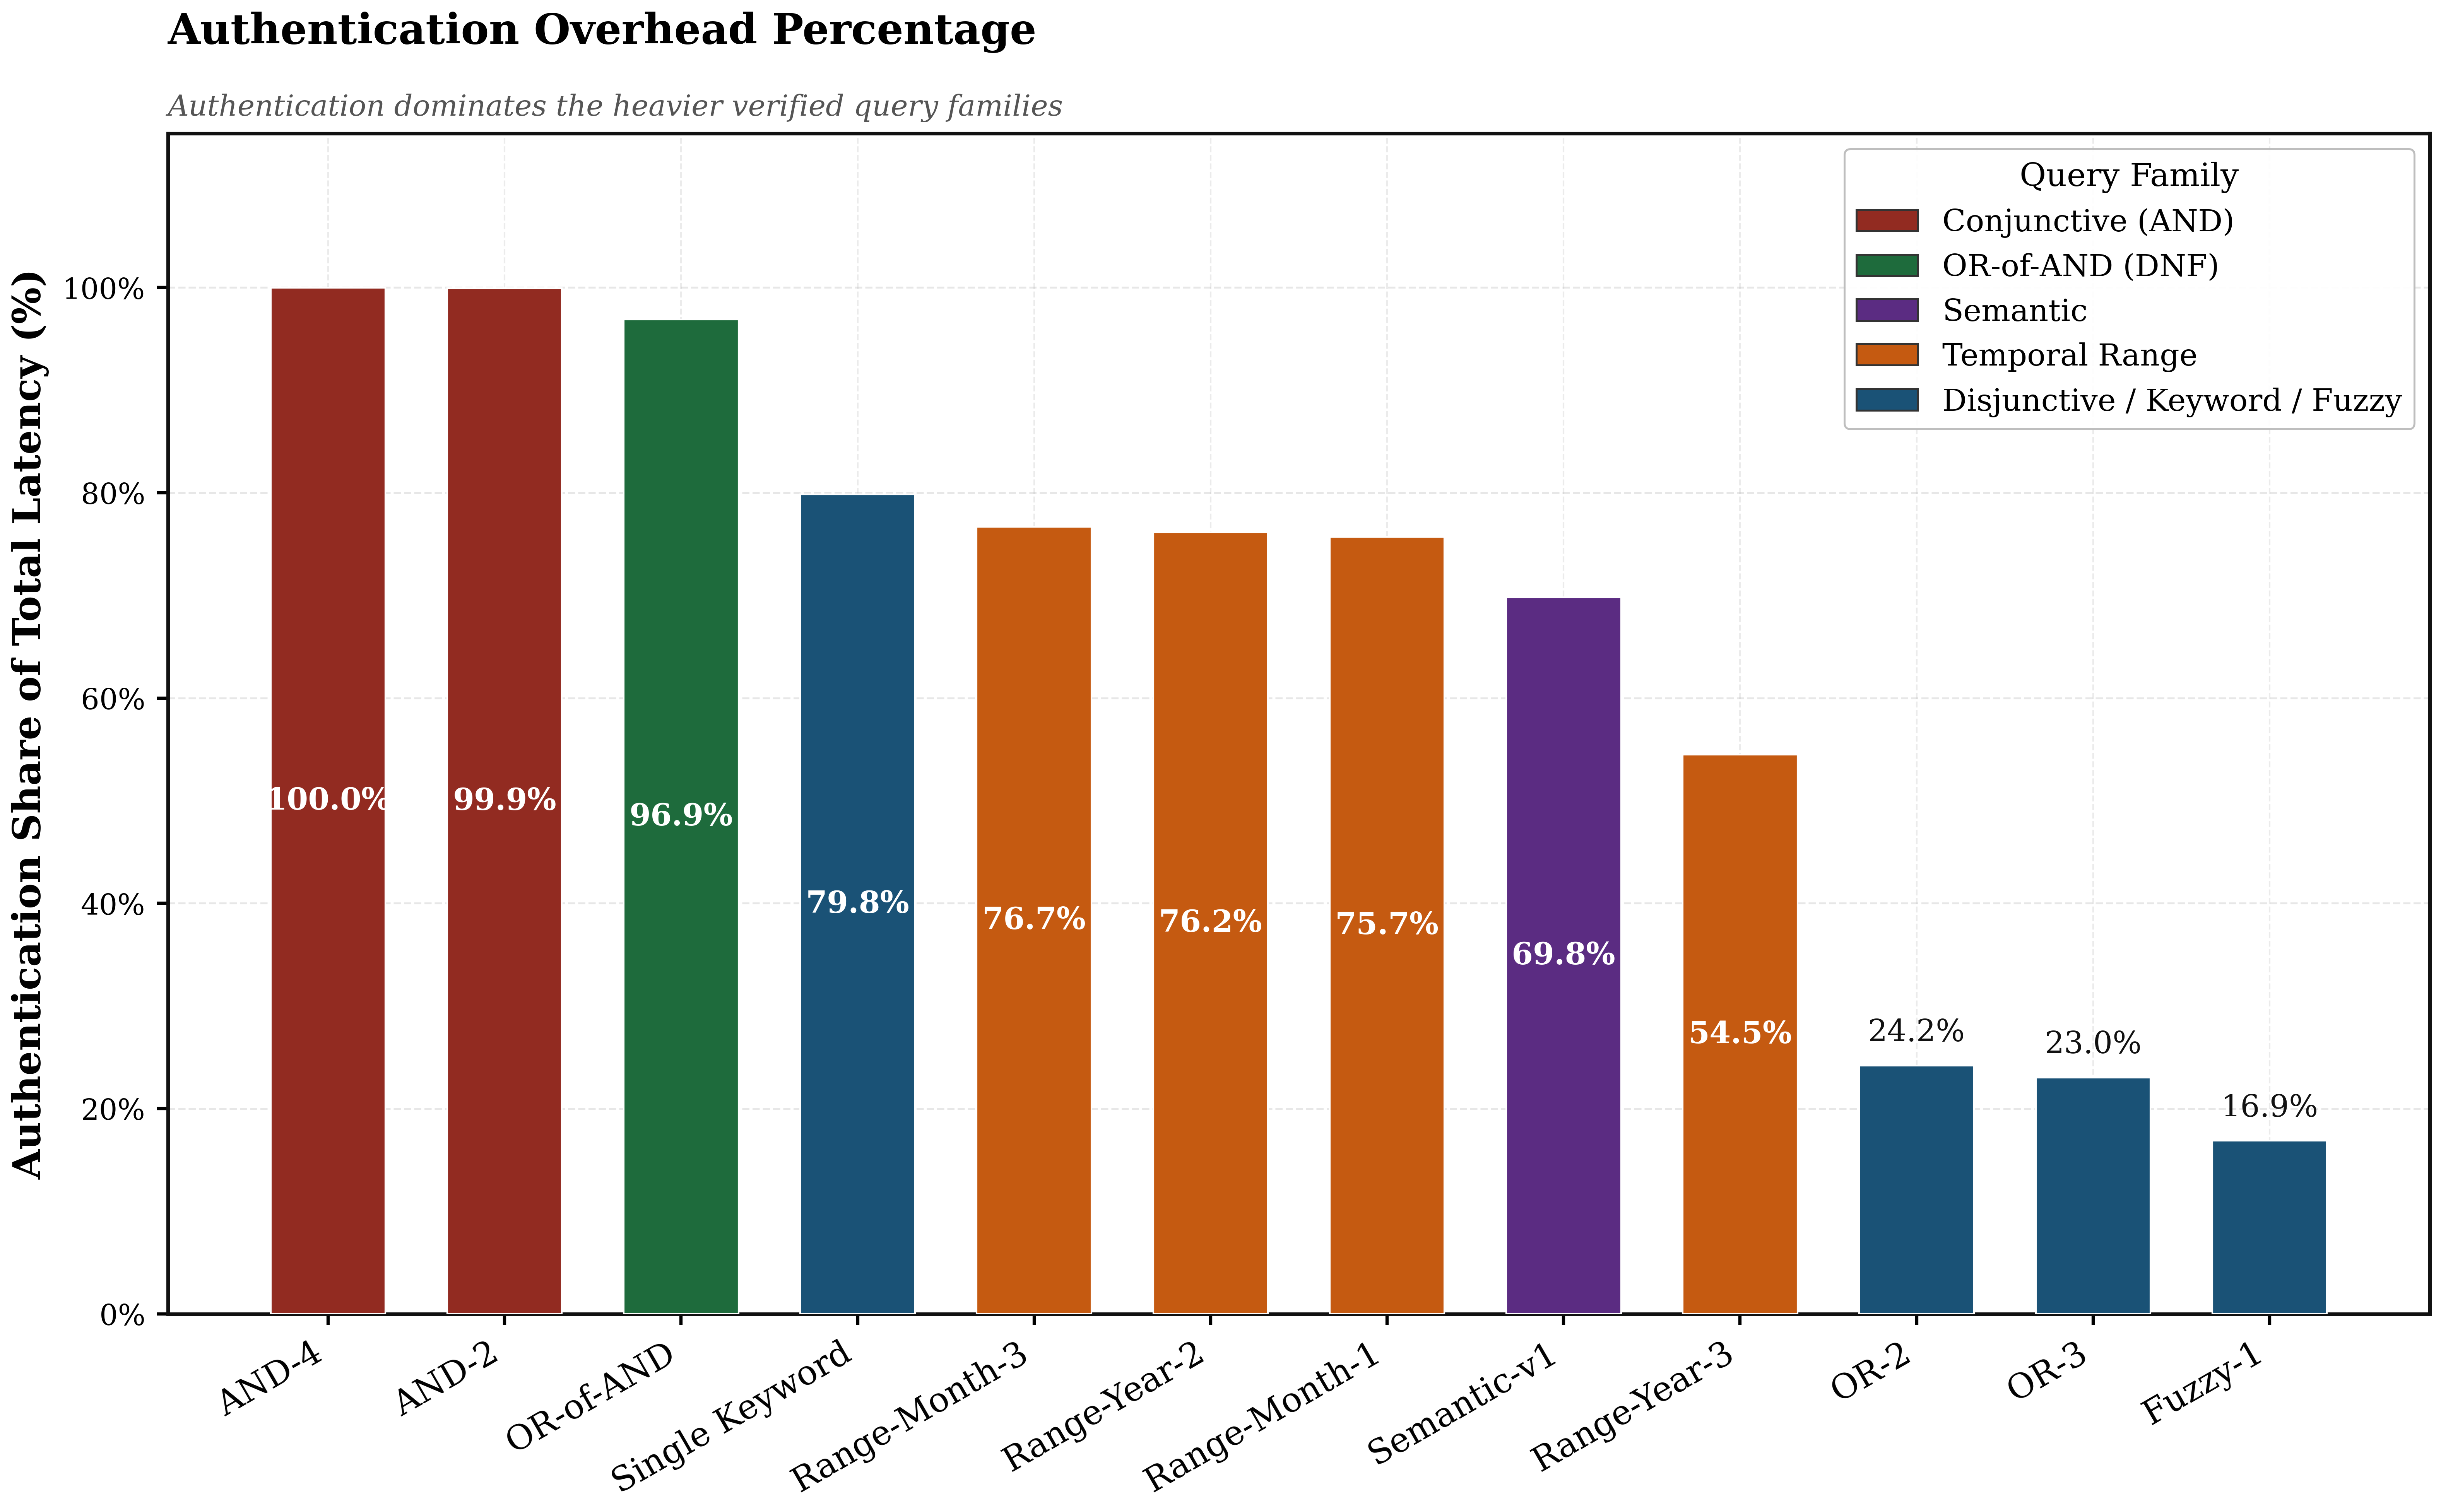
\includegraphics[width=0.48\textwidth]{pics/fig1_auth_overhead_pct.png}\hfill
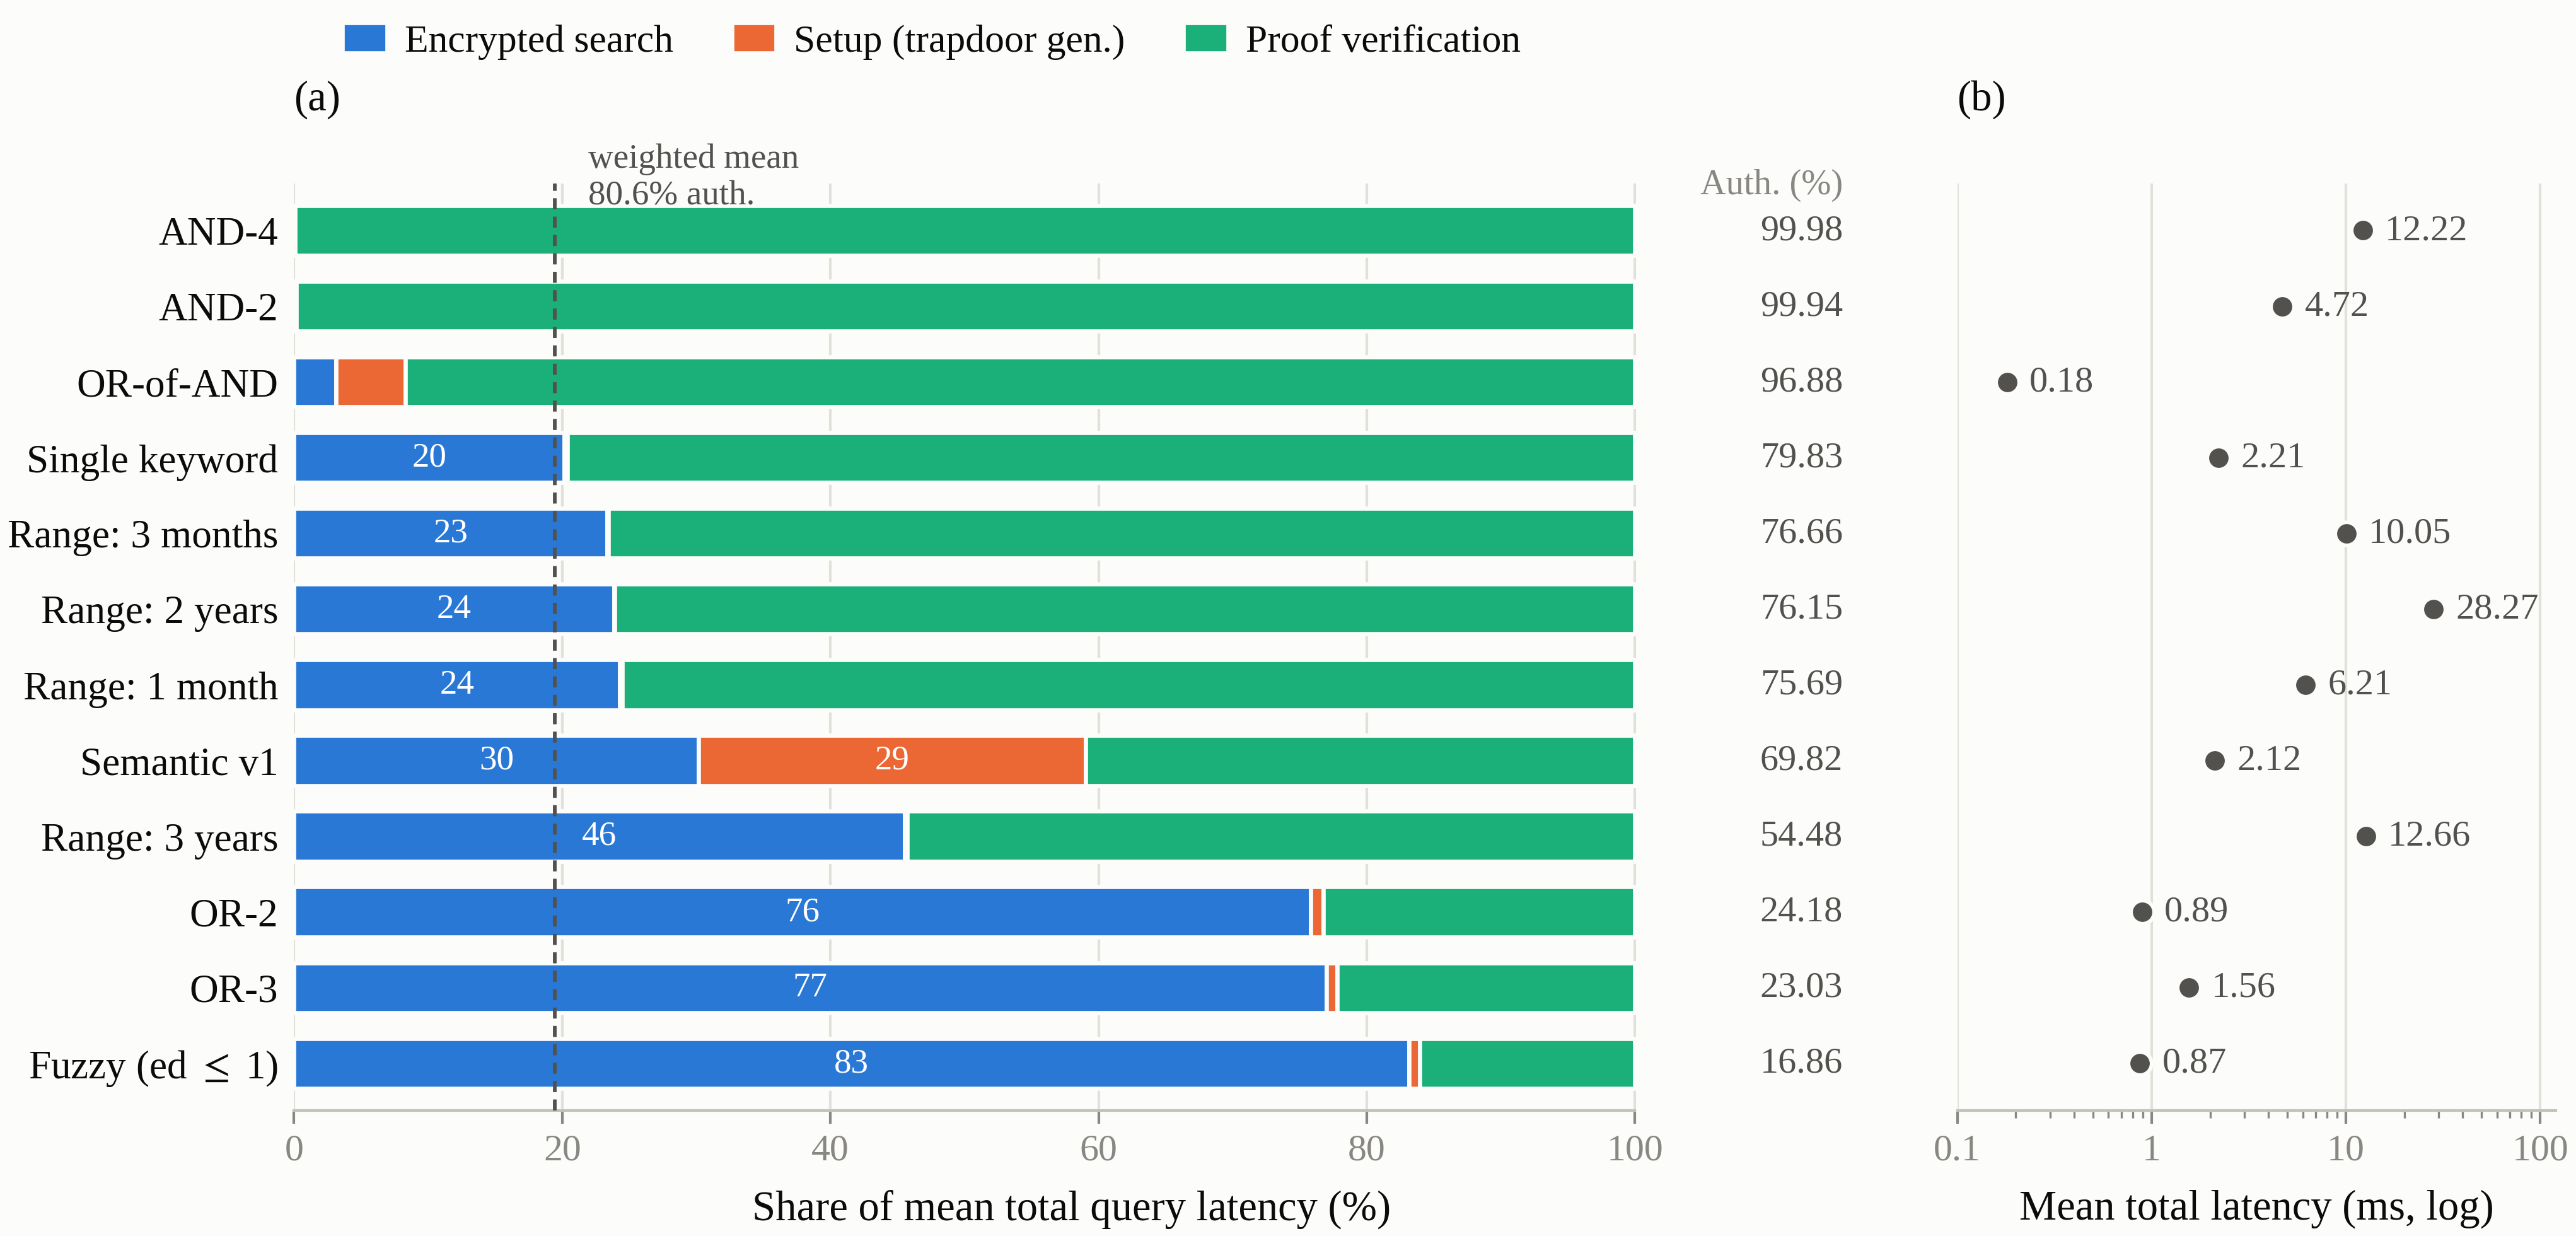
\includegraphics[width=0.48\textwidth]{pics/fig4_auth_share_horizontal.png}
\caption{Authentication share of total latency on the Enron-derived (left) and healthcare (right) tracks.}
\label{fig:authpct}
\end{figure*}

\subsection{Semantic-v1 Results}
\label{4E}

Semantic-v1 was evaluated on 12 concept-expanded workloads per corpus. Mean Enron latency was 755.8416~ms: 315.8987~ms for expansion setup, 71.2563~ms for search, and 368.6867~ms for verification. Healthcare latency was 12.6985~ms: 7.7169~ms for setup, 0.6275~ms for search, and 4.3540~ms for verification. The difference is driven by expansion breadth and posting-list length. These results characterize authenticated concept expansion over keyword postings, not embedding-based semantic retrieval.

\subsection{Healthcare-Corpus Validation}
\label{4F}

All 386 healthcare workloads completed without honest-server verification failures. The workload-weighted mean was 36.0062~ms, comprising 3.3046~ms of search and 32.4530~ms of verification. This aggregate is influenced by 240 single-keyword workloads; the 114 Boolean and fuzzy workloads averaged 5.0466~ms, close to the Enron result of 5.2503~ms.

\begin{table}[!tb]
\centering
\caption{Selected Healthcare Query-Family Means}
\label{tab:hc-family}
\setlength{\tabcolsep}{3pt}
\renewcommand{\arraystretch}{1.05}
\resizebox{\columnwidth}{!}{%
\begin{tabular}{lrrrr}
\toprule
\textbf{Query Type} &
\textbf{Count} &
\textbf{Total (ms)} &
\textbf{Search (ms)} &
\textbf{Verify (ms)} \\
\midrule
single\_keyword & 240 & 40.5753  & 2.5299  & 38.0396  \\
and\_2          & 24  & 3.2350   & 0.4235  & 2.8017   \\
and\_4          & 12  & 5.3278   & 0.1541  & 5.1575   \\
and\_6          & 6   & 7.8838   & 0.1821  & 7.6803   \\
and\_8          & 6   & 10.3833  & 0.2641  & 10.0932  \\
and\_10         & 6   & 13.0665  & 0.3526  & 12.6799  \\
or\_2           & 24  & 3.3355   & 0.7852  & 2.5404   \\
or\_3           & 12  & 5.5967   & 1.6782  & 3.9013   \\
or\_of\_and     & 12  & 6.7653   & 1.0907  & 5.6546   \\
fuzzy\_1        & 12  & 1.4450   & 0.1719  & 1.2672   \\
semantic\_v1    & 12  & 12.6985  & 0.6275  & 4.3540   \\
range\_month\_1 & 8   & 81.1254  & 13.6651 & 67.4517  \\
range\_month\_3 & 6   & 144.6576 & 24.5747 & 120.0662 \\
range\_year\_2  & 4   & 410.9589 & 70.5322 & 340.4091 \\
range\_year\_3  & 2   & 135.9195 & 25.5169 & 110.3744 \\
\bottomrule
\end{tabular}%
}
\end{table}

The similar Boolean costs across corpora indicate that \(k\) and \(s\), rather than total corpus size, dominate selective queries. In contrast, healthcare single-keyword and range queries are heavier because their posting lists are longer. Verification contributes 90.13\% of healthcare latency, consistent with Fig.~\ref{fig:authpct}.

\subsection{Same-Stack SeaCQ Comparison}
\label{4G}

SeaCQ's conjunctive path was reimplemented using the same host, Node.js runtime, inverted indexes, warm-up protocol, and cached witnesses. The implementations share the OXT-style search path but differ in verification: SeaCQ checks every returned document in every contributing list, whereas PrivSearch checks at most \(s=5\). Their accumulator work is therefore
\begin{equation}
\frac{\text{SeaCQ operations}}{\text{PrivSearch operations}}
=
\frac{|R|k}{\min(s,|R|)k}
=
\frac{|R|}{s},
\qquad |R|>s.
\label{eq:opsratio}
\end{equation}
The operation-count ratio is independent of \(k\) and hardware. Enron SeaCQ latency was measured directly; healthcare SeaCQ latency was derived from exact operation counts and the measured \(t_{exp}=174.0~\text{\textmu s}\).

\begin{table}[!tb]
\centering
\caption{Same-Stack Conjunctive Comparison}
\label{tab:seacq}
\setlength{\tabcolsep}{2.8pt}
\renewcommand{\arraystretch}{1.06}
\resizebox{\columnwidth}{!}{%
\begin{tabular}{llrrrrrr}
\toprule
\textbf{Corpus} & \textbf{\(k\)} & \textbf{\(|\bar R|\)} &
\makecell[r]{\textbf{PS}\\\textbf{ops}} &
\makecell[r]{\textbf{SQ}\\\textbf{ops}} &
\makecell[r]{\textbf{Ops}\\\textbf{ratio}} &
\makecell[r]{\textbf{PS Ver.}\\\textbf{(ms)}} &
\makecell[r]{\textbf{SQ Ver.}\\\textbf{(ms)}} \\
\midrule
Enron  & 2  & 10.3  & 10 & 20.7   & \(2.1\times\)   & 2.446  & 5.215 \\
Enron  & 4  & 10.3  & 20 & 41.3   & \(2.1\times\)   & 5.110  & 10.374 \\
Enron  & 6  & 10.0  & 30 & 60.0   & \(2.0\times\)   & 7.717  & 15.261 \\
Enron  & 8  & 10.0  & 40 & 80.0   & \(2.0\times\)   & 10.043 & 19.812 \\
Enron  & 10 & 10.0  & 50 & 100.0  & \(2.0\times\)   & 12.487 & 24.805 \\
\midrule
Health & 2  & 102.0 & 10 & 204.0  & \(20.4\times\)  & 3.106  & 35.504\(^{\ddagger}\) \\
Health & 4  & 60.3  & 20 & 241.3  & \(12.1\times\)  & 5.497  & 42.002\(^{\ddagger}\) \\
Health & 6  & 379.7 & 30 & 2278.0 & \(75.9\times\)  & 8.544  & 396.463\(^{\ddagger}\) \\
Health & 8  & 922.7 & 40 & 7381.3 & \(184.5\times\) & 11.292 & 1284.647\(^{\ddagger}\) \\
Health & 10 & 918.7 & 50 & 9186.7 & \(183.7\times\) & 13.680 & 1598.847\(^{\ddagger}\) \\
\bottomrule
\end{tabular}%
}
\vspace{2pt}

\parbox{\columnwidth}{\footnotesize
PS: PrivSearch with \(s=5\); SQ: exhaustive SeaCQ-style verification.
Operations are 2048-bit modular exponentiations. Enron SQ latency was measured; \(^{\ddagger}\)healthcare SQ latency was derived as
\(|\bar R|kt_{exp}\). Witnesses were precomputed for both systems.}
\end{table}

Enron produced a stable \(2.0\)--\(2.1\times\) reduction because \(|\bar R|\approx10\). Healthcare ratios ranged from \(12.1\times\) to \(184.5\times\) because its result sets were larger. PrivSearch verification remained approximately linear in \(k\) but bounded in \(|R|\); when \(|R|\leq s\), both approaches perform the same accumulator work.

This efficiency has a corresponding soundness cost. For the healthcare \(k=10\) row, checking 5 of 918.7 results reduces accumulator work by \(183.7\times\) but detects a single invalid result with probability only \(5/918.7\approx0.54\%\). Thus, Eq.~\eqref{eq:opsratio} and Theorem~\ref{thm:sampled} describe opposite sides of the same trade-off.

\subsection{Literature-Based Comparison}
\label{4H}

Table~\ref{tab:related_comparison} provides the broader comparison. TELEX supports rich private queries but assumes trusted hardware; EAQ provides authenticated multiattribute retrieval without query-content privacy; VQL verifies off-chain queries without privacy-preserving search; and MSTDB supports hybrid semantic queries without authenticated private retrieval. Because these systems were not reproduced on the same stack, no numerical performance superiority is claimed.

\subsection{Statistical Significance}
\label{4I}

Latency distributions for high-cardinality workloads were strongly right-skewed. For example, Enron \texttt{single\_keyword} had a mean of 17.9511~ms and median of 3.6704~ms, while \texttt{range\_year\_2} had a mean of 1{,}329.7822~ms and median of 383.6428~ms. We therefore use bootstrap rather than normal-approximation intervals. Boolean workloads were substantially less skewed because their sampled-verification cost is primarily governed by \(k\) and \(s\).

\begin{table}[!tb]
\centering
\caption{Selected Statistical Comparisons}
\label{tab:sig}
\scriptsize
\setlength{\tabcolsep}{3pt}
\begin{tabular}{p{2.9cm}rrl}
\toprule
\textbf{Comparison} & \textbf{\(p\)-value} &
\textbf{Cliff's \(\delta\)} & \textbf{Sig.} \\
\midrule
Enron \texttt{single\_keyword} vs.\ \texttt{and\_2}
& 0.0029 & \(+0.223\) & yes \\

Enron \texttt{and\_2} vs.\ \texttt{and\_10}
& \(<0.0002\) & \(-1.000\) & yes \\

Enron \texttt{and\_2} vs.\ \texttt{or\_2}
& 0.3105 & \(-0.045\) & no \\

Healthcare \texttt{and\_2} vs.\ \texttt{or\_2}
& 0.9453 & \(+0.313\) & no \\

Healthcare \texttt{semantic\_v1} vs.\ \texttt{fuzzy\_1}
& \(<0.0002\) & \(+0.986\) & yes \\

Enron \texttt{and\_2} vs.\ Healthcare \texttt{and\_2}
& \(<0.0002\) & \(-0.606\) & yes \\
\bottomrule
\end{tabular}
\end{table}

The \(k=2\) versus \(k=10\) comparison showed complete separation (\(\delta=-1.000\)), supporting linear growth with clause count. By contrast, AND and OR did not differ significantly on either corpus, consistent with their similar accumulator-operation counts. Healthcare \(k=2\) conjunctions were modestly but significantly slower than their Enron counterparts. Statistical power is determined by the number of independent workloads, not the 100 repeated trials; small family-level effects should therefore be interpreted cautiously.

\subsection{Ablation Study}
\label{4J}

The ablation progressed from plaintext postings (A0) through encrypted retrieval (A1), authenticated conjunction (A2), OR/OR-of-AND (A3), range processing (A4), replay protection (A5), and the integrated system (A6/A6b). Encryption increased latency from 0.0232 to 1.0731~ms, whereas authentication increased it to 100.5184~ms, including 99.4453~ms of verification. OR support added 3.7714~ms. The range stage reached 3{,}893.8788~ms because of its large result set, while replay checking added only 0.0205~ms for acceptance and 0.0036~ms for rejection. The ablation used 10 trials per query in one session and supports relative component attribution; Tables~\ref{tab:enron-summary} and~\ref{tab:hc-family} remain authoritative for absolute performance.

\subsection{Resource and Storage Overhead}
\label{4K}

Resource measurements cover 53 Enron-side workloads with three trials each.

\begin{table}[!tb]
\centering
\caption{Global Deployment-Cost Summary}
\label{tab:resource}
\small
\begin{tabular}{lr}
\toprule
\textbf{Metric} & \textbf{Value} \\
\midrule
Prepared posting sets & 102 \\
Indexed document references & 1{,}279{,}790 \\
Raw postings bytes & 37{,}164{,}996 \\
Encrypted payload bytes & 74{,}339{,}172 \\
Encrypted index size bytes & 74{,}434{,}355 \\
Blockchain commitment bytes & 74{,}101 \\
Storage overhead \(\rho_{storage}\) & \(2.0028\times\) \\
\bottomrule
\end{tabular}
\end{table}

The encrypted index approximately doubles raw posting storage, while blockchain commitments occupy only \(9.95\times10^{-4}\) of the encrypted-index size. Mean proof size ranges from 966~bytes for single-keyword and range queries to 7{,}216~bytes at \(k=10\), growing with clause count but remaining bounded by \(s\). CPU and memory values are process-level deltas; proof, commitment-reference, and network sizes are serialized-payload estimates rather than packet-capture measurements.

\subsection{Cryptographic Overhead}
\label{4L}

Across all 448 Enron workloads, cryptographic operations contributed 95.68\% of mean latency. Proof verification alone accounted for 48.1446~ms, or 73.62\% of the 65.3992~ms workload-weighted total. On healthcare, the cryptographic and proof-verification shares were 99.30\% and 90.13\%, respectively. Trapdoor generation and proof construction remained below 0.06~ms per family; encrypted-posting retrieval became substantial only for range and semantic-v1 queries. Inline commitment-reference checking contributed no measurable query-path latency, consistent with Theorem~\ref{thm:latsep}.

\begin{figure*}[!t]
\centering
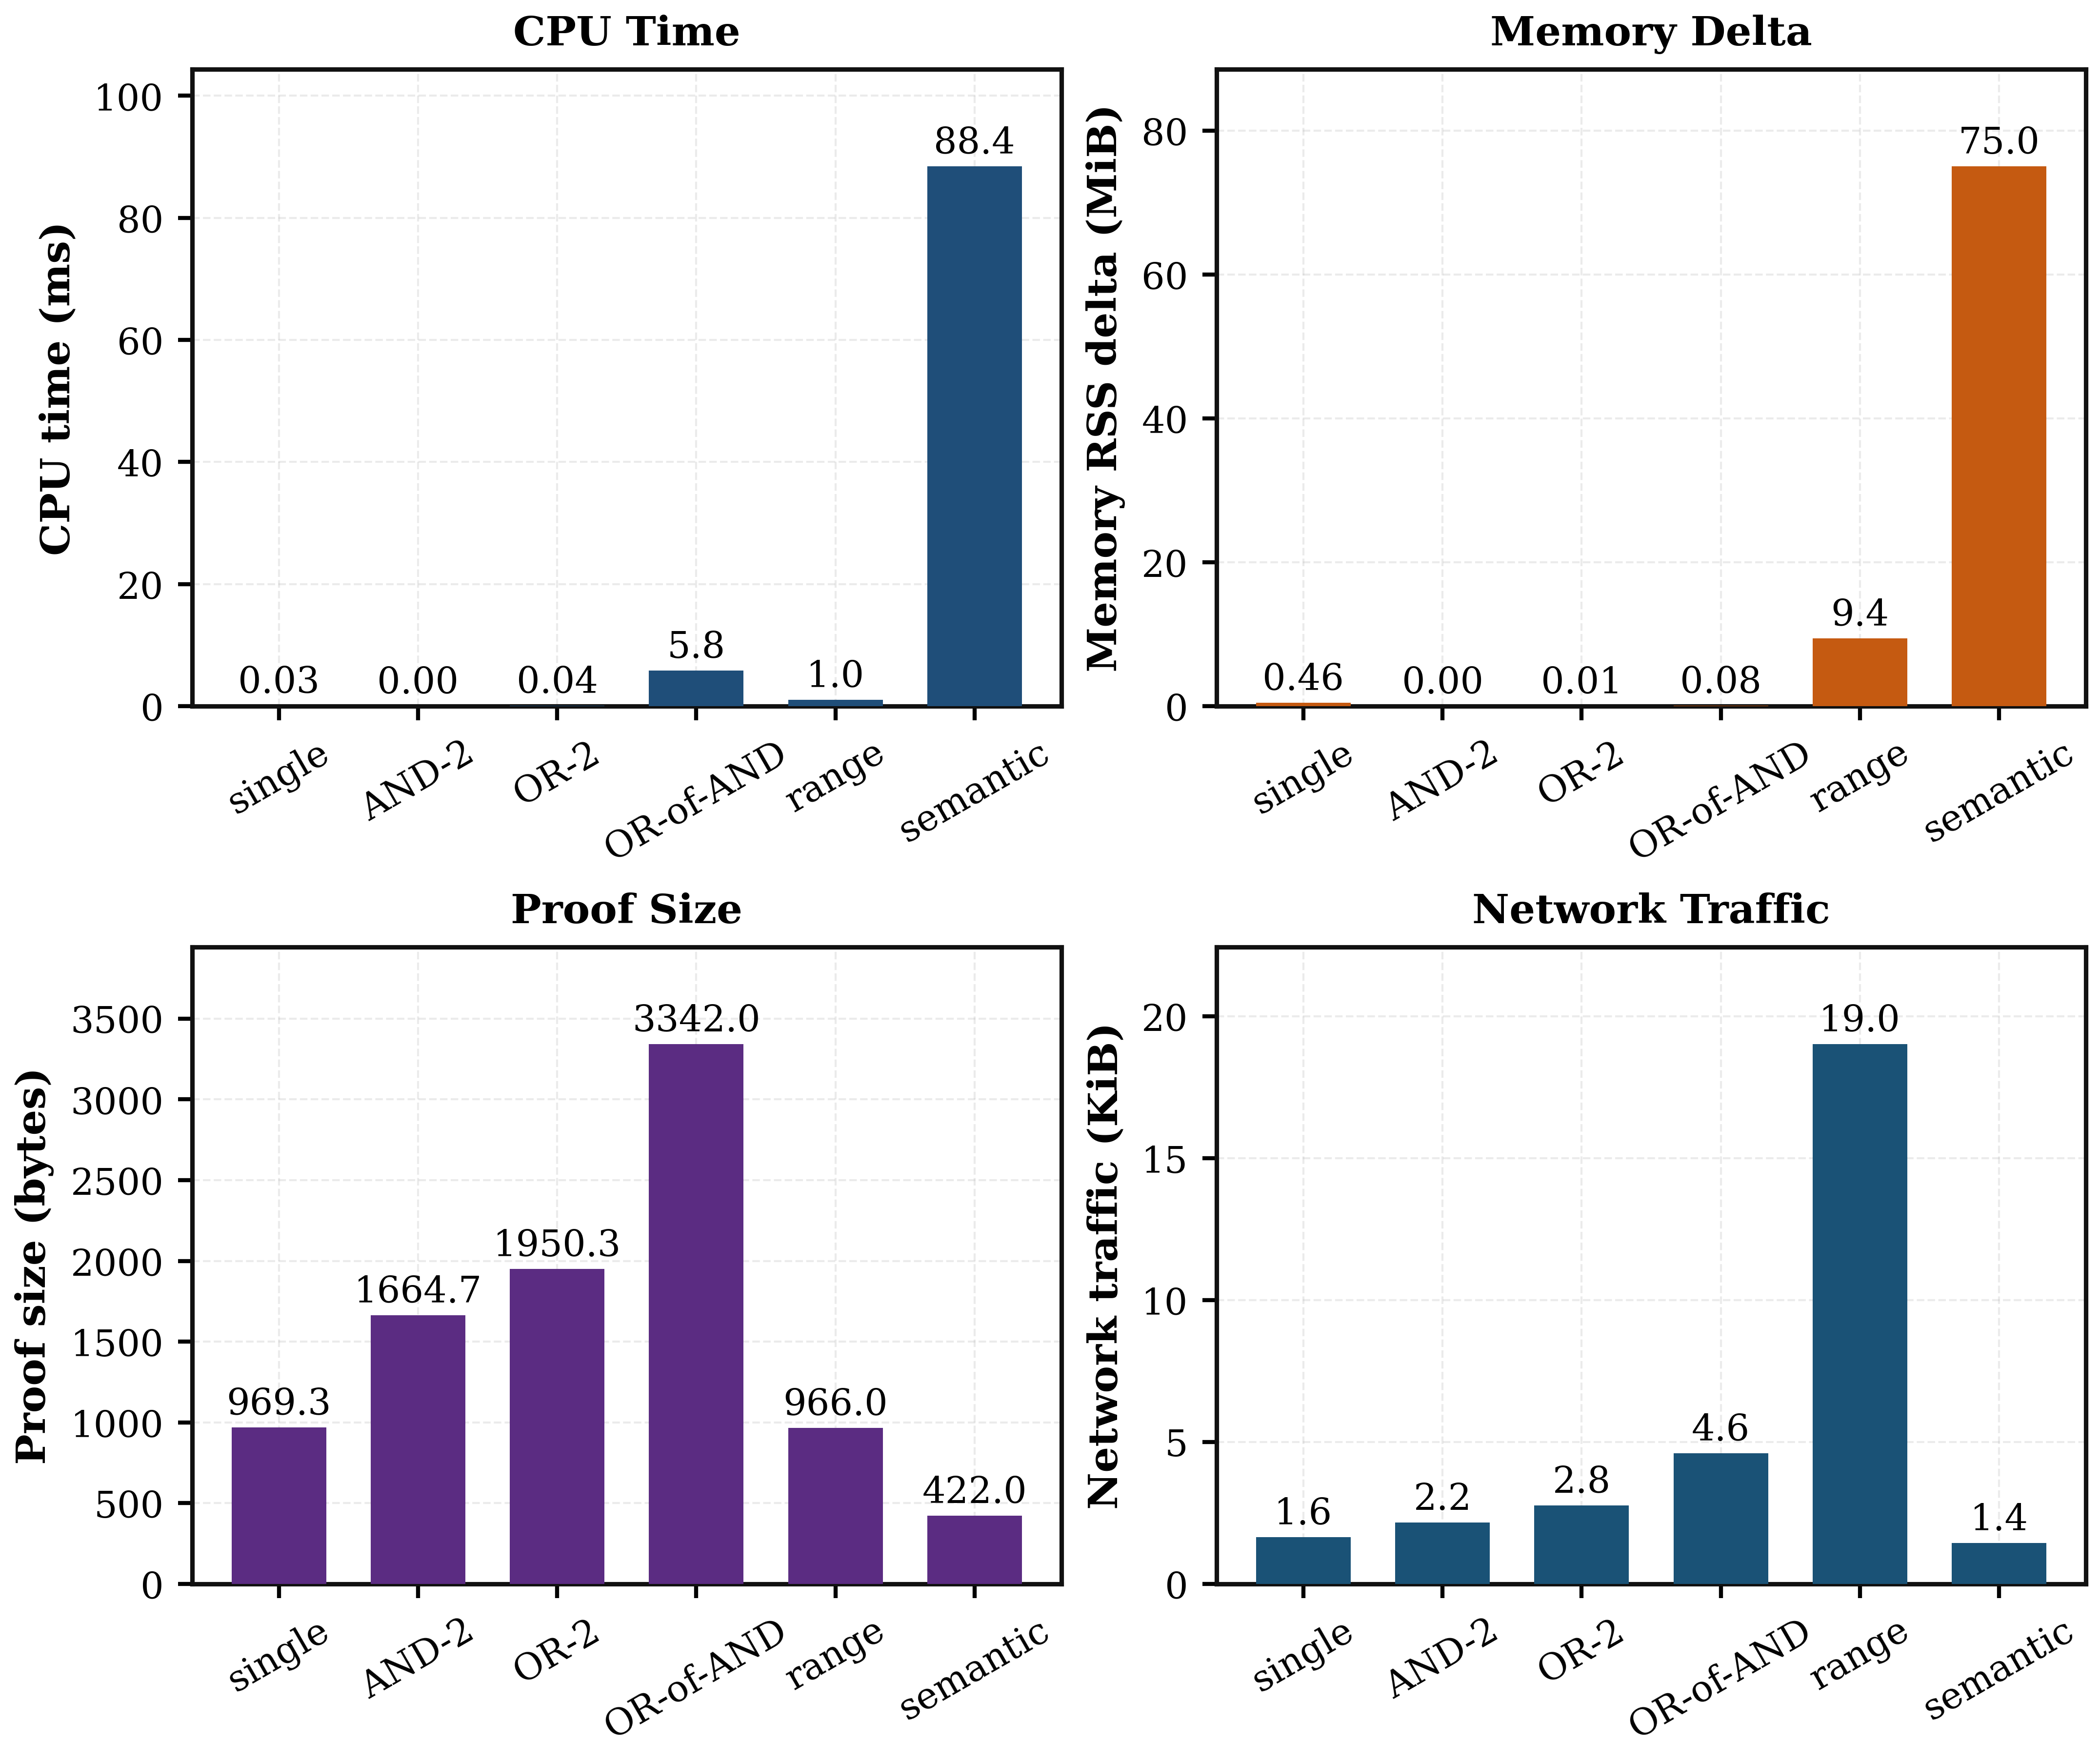
\includegraphics[width=0.48\textwidth]{pics/fig2_resource_overhead.png}\hfill
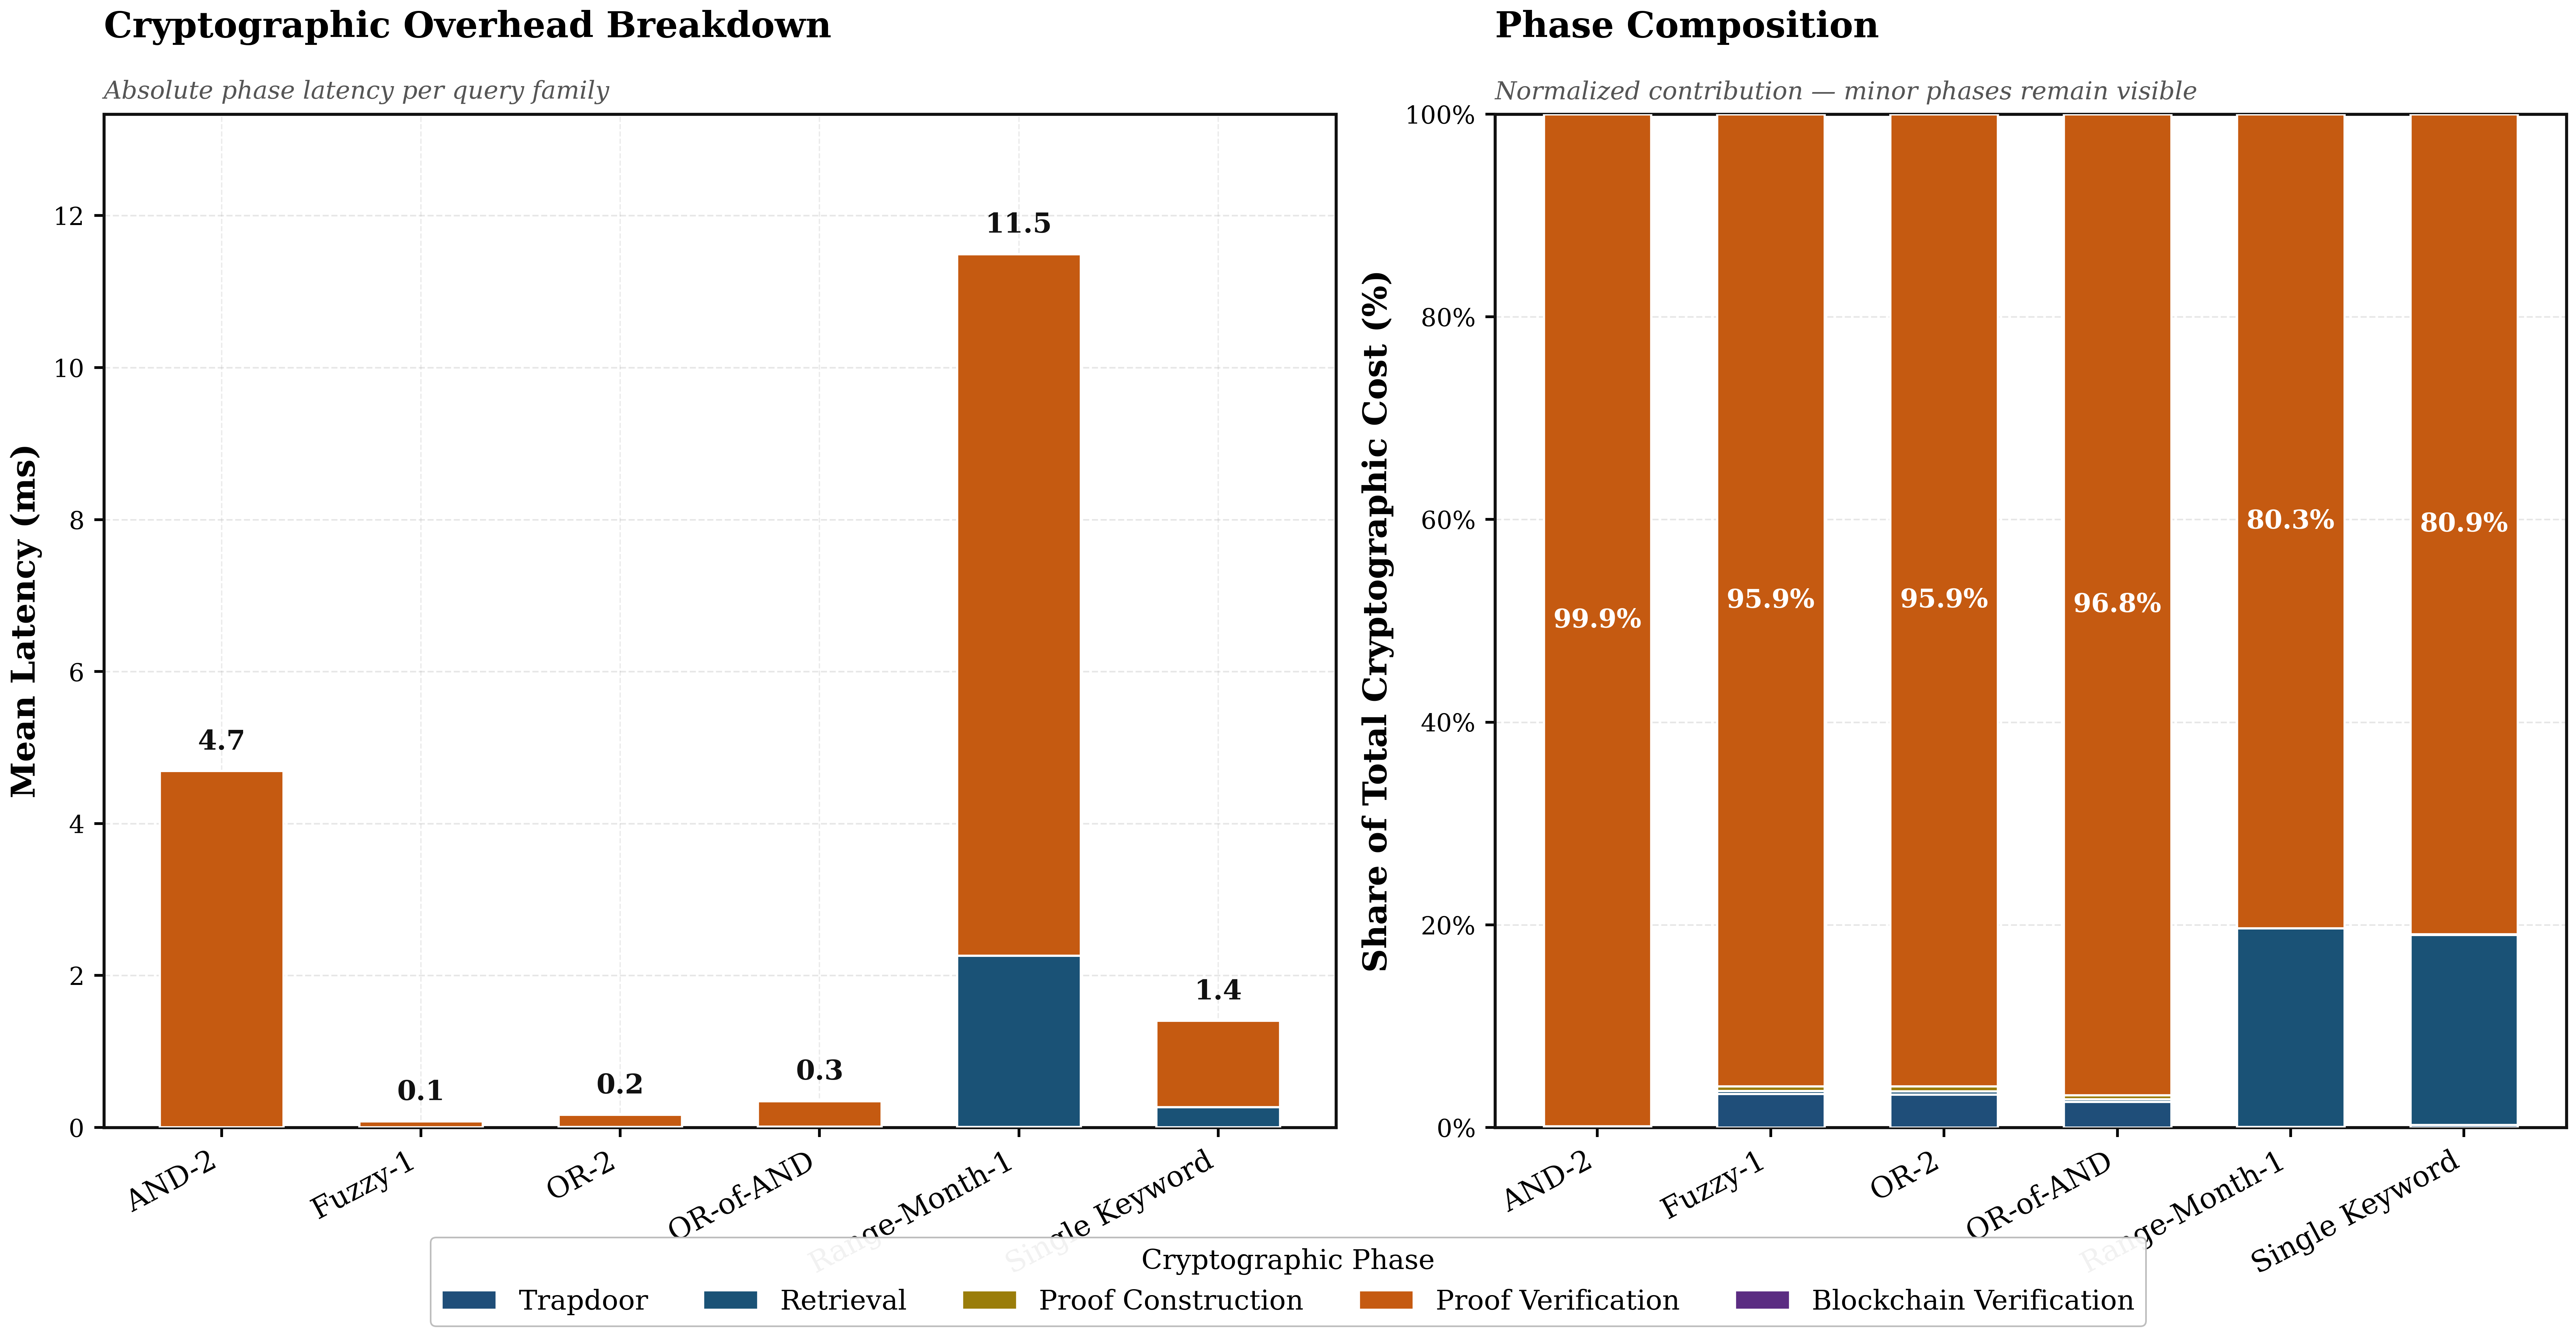
\includegraphics[width=0.48\textwidth]{pics/fig8_crypto_breakdown.png}
\caption{Resource overhead by query family (left) and latency decomposition by pipeline stage (right).}
\label{fig:crypto}
\end{figure*}

\subsection{Scalability}
\label{4M}

\textbf{Posting-list size.}
Mean latency increased from 2.6901~ms for lists of 1--10 documents to 4{,}829.4158~ms above 10{,}001 documents. Verification contributed 4{,}003.51~ms in the largest bucket, confirming that result-set processing remains linear in \(|R|\). Proof size remained nearly constant at 970--982~bytes because only \(s\) witnesses were transmitted.

\textbf{Clause count.}
Conjunctive latency increased from 2.5961~ms at two clauses to 13.6511~ms at ten clauses, approximately 1.38~ms per additional clause. Proof size increased from 1{,}670 to 7{,}212~bytes. Disjunctive and DNF workloads followed the same trend.

\textbf{Concurrency.}
Concurrency levels of 1, 5, 10, and 25 achieved 100\% success without
measured queueing or latency inflation.  For the representative authenticated
conjunctive family (AND-2), throughput remained approximately 379--400\,req/s,
indicating stable but primarily serialized verification rather than multicore
scaling.  Simpler query families (e.g., range queries) achieve higher
per-server throughput; AND-2 represents the typical authenticated-search
workload.  Horizontal scaling requires multi-process workers and a shared
nonce registry.

\begin{figure*}[!t]
\centering
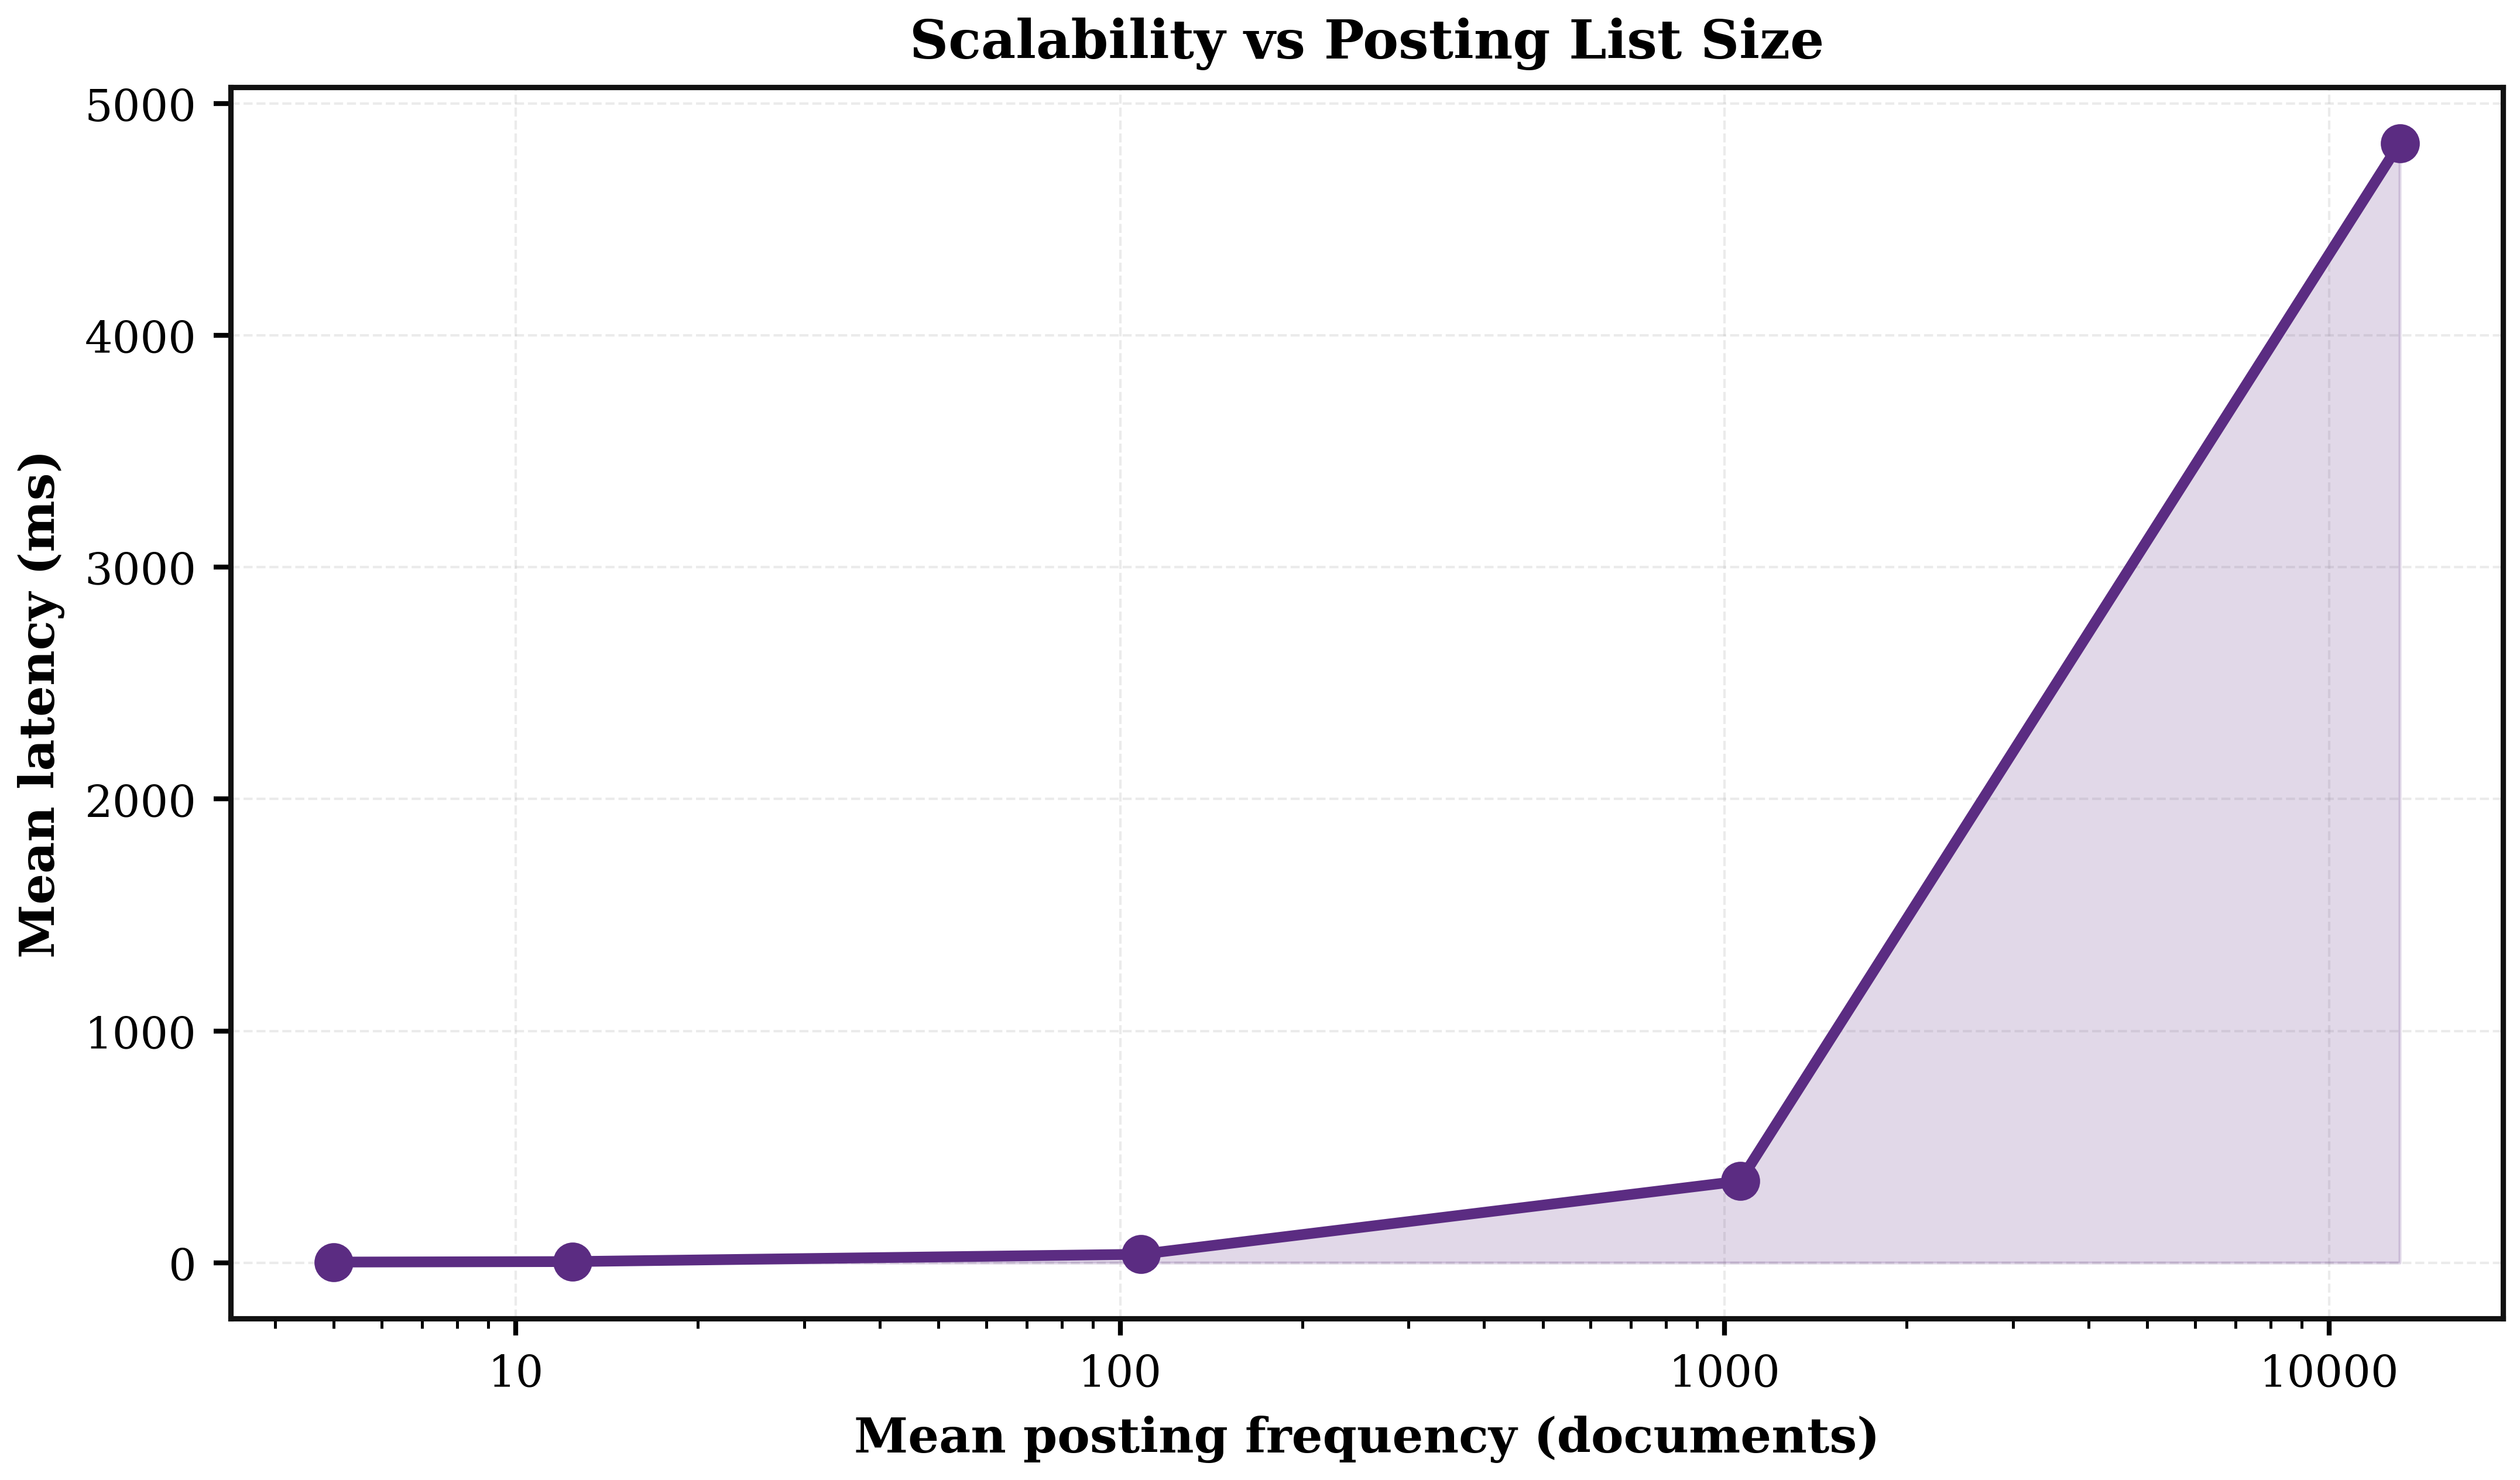
\includegraphics[width=0.42\textwidth]{pics/fig5_scalability_posting_list.png}\hfill
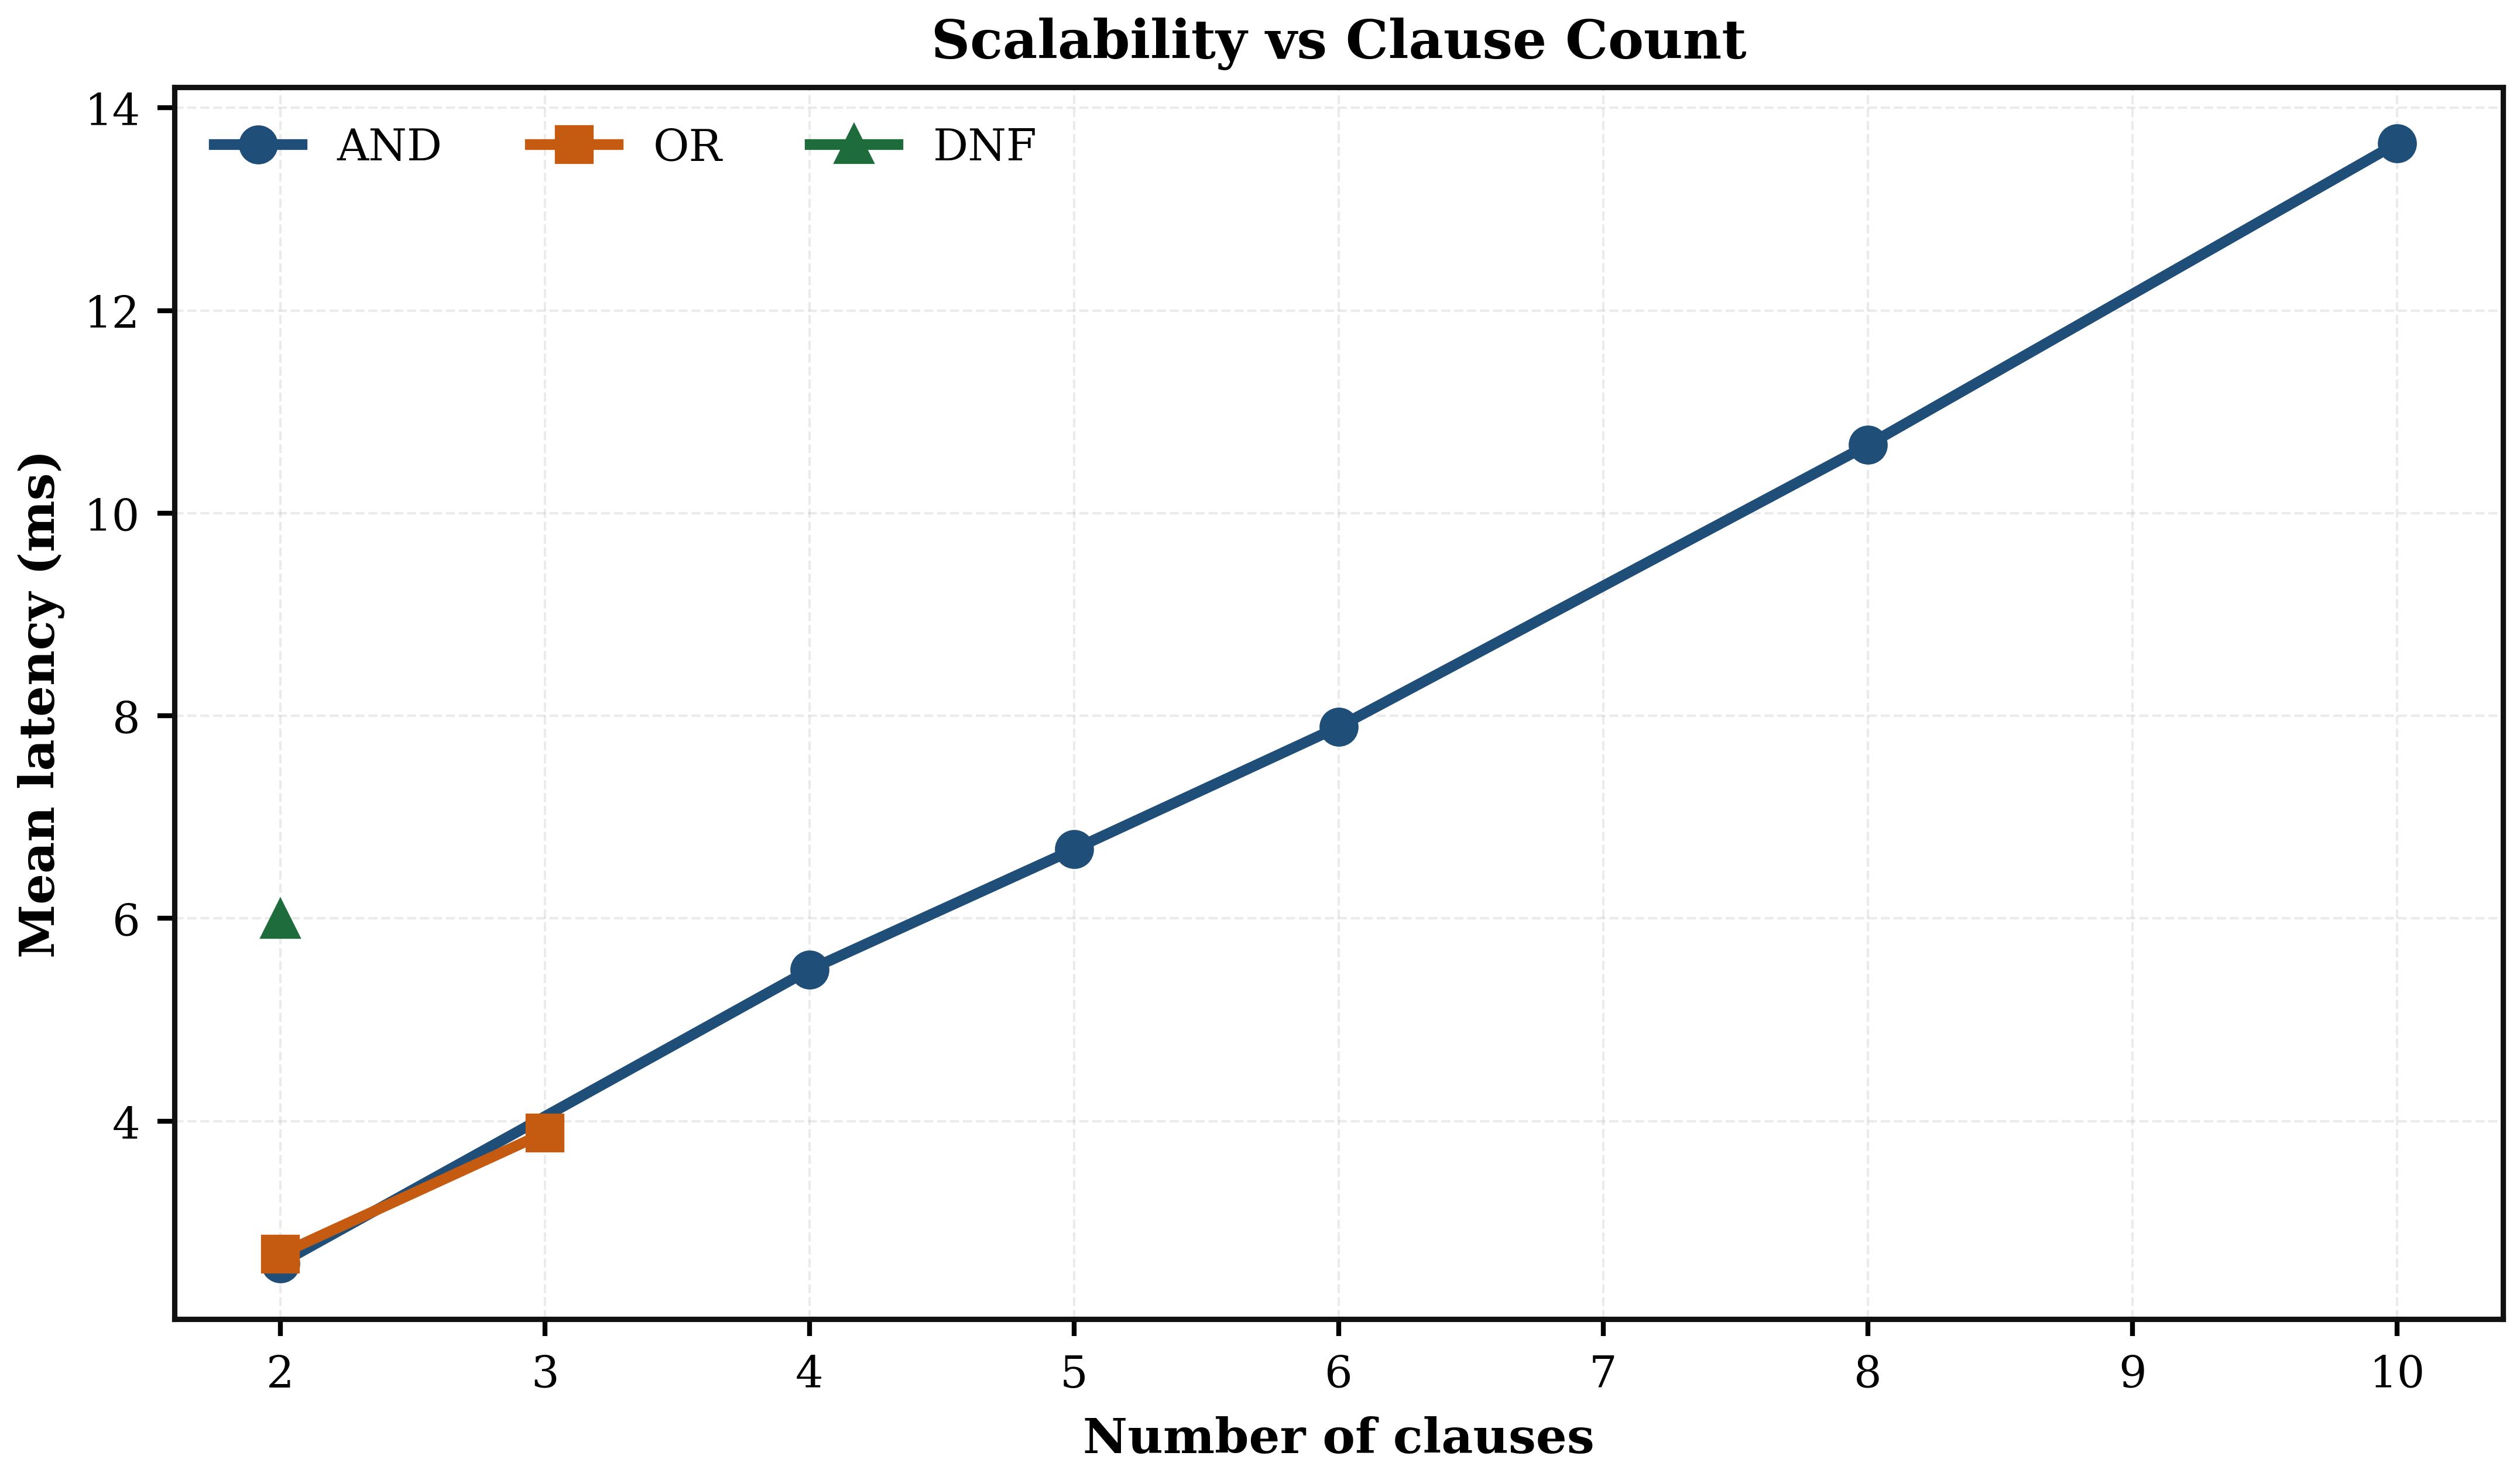
\includegraphics[width=0.42\textwidth]{pics/fig6_scalability_clause_count.png}\hfill
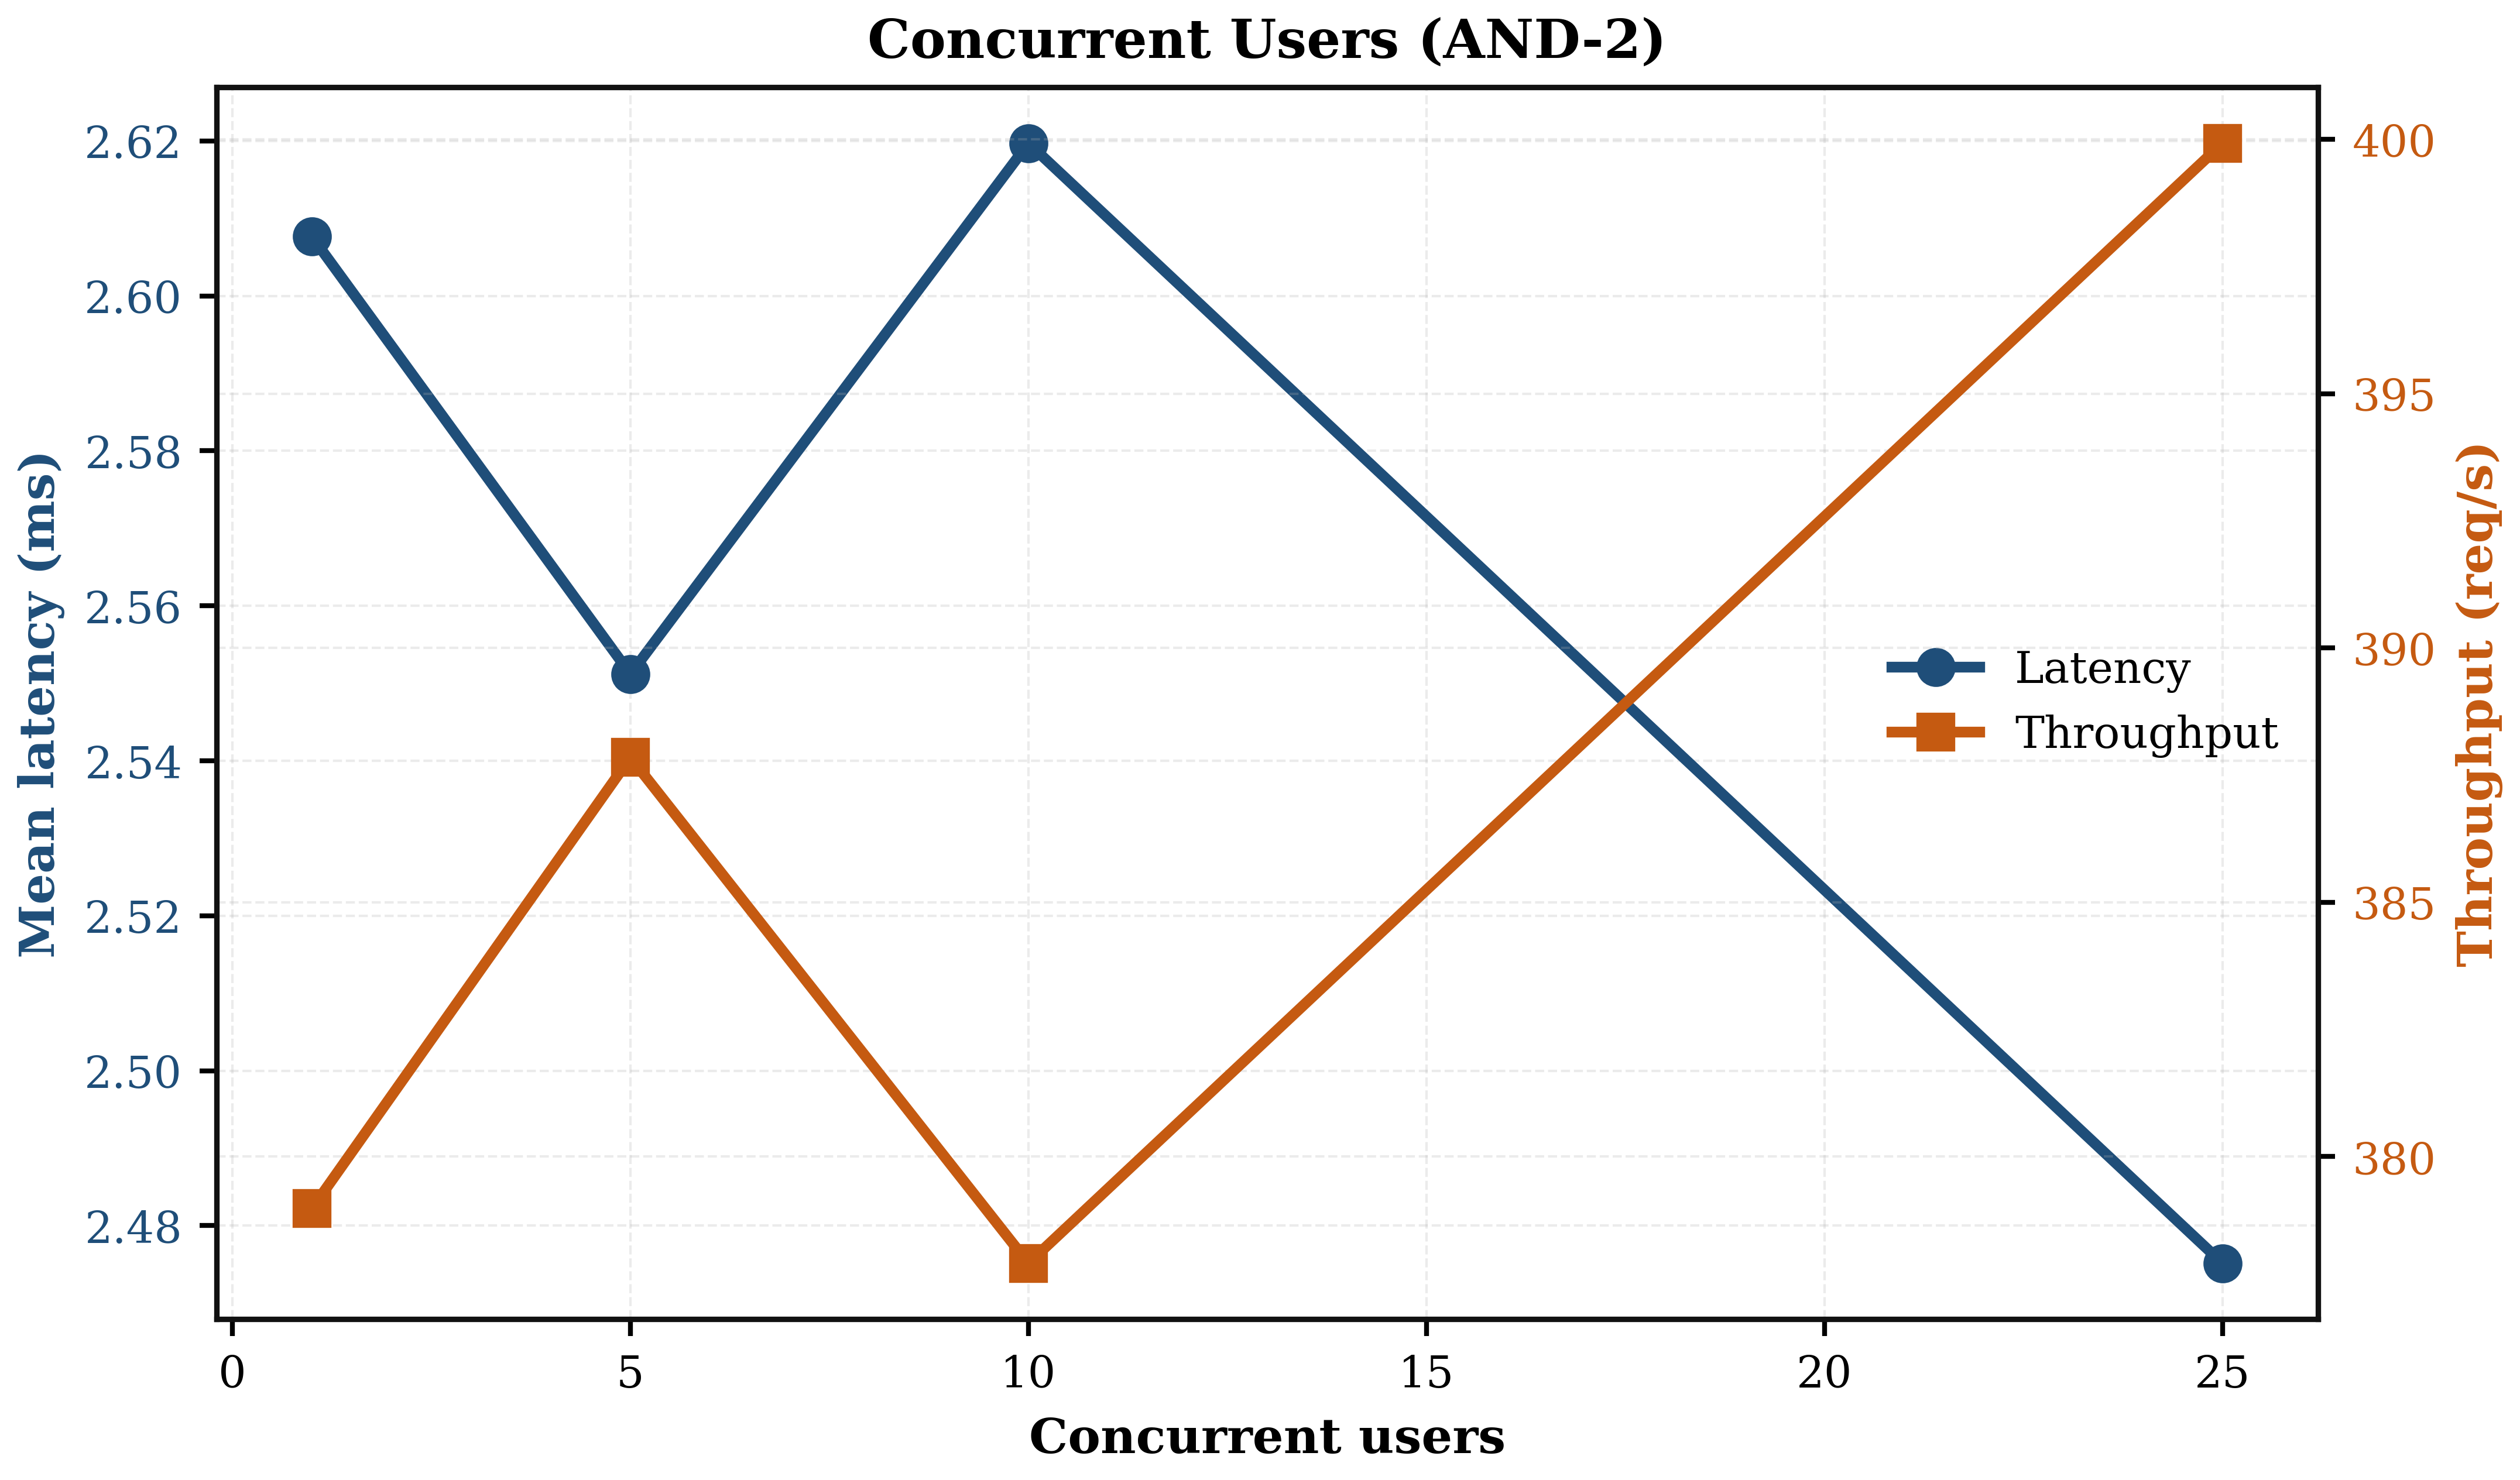
\includegraphics[width=0.42\textwidth]{pics/fig7_concurrent_users.png}
\caption{Scalability with posting-list size (left), clause count (centre), and concurrency (right, AND-2 representative).}
\label{fig:scale}
\end{figure*}

\subsection{Replay and Stale-Proof Protection}
\label{4N}

Across 200 live-API tests, PrivSearch accepted all first requests and rejected all 200 replays. Mean replay-rejection latency was 0.7897~ms (P95: 1.1734~ms), compared with 581.4113~ms for an accepted authenticated write. The in-process registry check accounted for 0.0036~ms; the remaining rejection time arose from HTTP handling. The experiment used required mode, a 300~s TTL and clock-skew allowance, and 200 resident keys. Capacity-pressure and restart behavior were not evaluated; the guarantee remains subject to Corollary~\ref{cor:evict}.

Each proof also contains its index-state root. Before witness verification, the client compares this root with the current \(\mathrm{Com}(I)\); a proof from a superseded state therefore fails immediately. This stale-proof mechanism is implemented but was not evaluated through a dedicated injection experiment.

\subsection{Tamper-Detection Efficacy}
\label{4Ntd}

We substituted \(t\in\{1,2,5,10\}\) fabricated identifiers into legitimate result sets and sampled \(s\in\{5,10,25,50\}\) returned documents. Each \((t,s)\) configuration was evaluated over 100 trials in small, medium, and large result-set strata. Detection occurs when at least one fabricated identifier is sampled.

\begin{table}[!tb]
\centering
\caption{Empirical tamper-detection rates and corrected theoretical probability
$\bar{p}_{\rm det}$: 11 representative cells from the 48-cell
$(t,s)\times\text{bucket}$ matrix ($N{=}100$ trials each).
$\bar{p}_{\rm det}=\tfrac{1}{N}\sum_i p_{\rm det}(n_i,t,s)$ averages over
the $N$ actual workload result sizes $n_i$ in each bucket, replacing the
prior practice of evaluating only at the bucket mean $\bar{R}$.
Empirical 95\,\% CIs use the Wilson interval.}
\label{tab:tamper}
\small
\begin{tabular}{ccrr r r}
\toprule
$t$ & $s$ & Bucket & $\bar{R}$ &
Empirical [\,95\,\% CI\,] & $\bar{p}_{\rm det}$ \\
\midrule
1 &  5 & small  &   20 & 40\% [31,\,50] & 35.1\% \\
1 & 10 & small  &   20 & 68\% [58,\,76] & 62.7\% \\
1 & 25 & small  &   20 & 95\% [89,\,98] & 92.3\% \\
5 &  5 & small  &   21 & 76\% [67,\,83] & 80.9\% \\
10 & 5 & small  &   24 & 95\% [89,\,98] & 92.8\% \\
\midrule
1 &  5 & medium &  167 & 4\% [2,\,10]   &  4.3\% \\
5 & 25 & medium &  167 & 62\% [52,\,71] & 64.0\% \\
10 & 50 & medium & 167 & 95\% [89,\,98] & 94.6\% \\
\midrule
1 &  5 & large  & 3603 & 0\% [0,\,4]    &  0.3\% \\
1 & 50 & large  & 3603 & 2\% [1,\,7]    &  3.0\% \\
10 & 50 & large & 3603 & 22\% [15,\,31] & 24.2\% \\
\bottomrule
\end{tabular}
\end{table}

Across the complete 48-cell matrix, the mean absolute difference between
empirical and $\bar{p}_{\rm det}$ is 2.2 percentage points, down from
4.0\,pp when theory was evaluated only at $\bar{R}$.  The correction is most
visible in the small-bucket row where $s{=}25$, $\bar{R}{=}20$: evaluating at
the mean gave $p_{\rm det}(20,1,25){=}100\,\%$ (because $s{>}\bar{R}$), yet
the empirical rate was $95\,\%$ and $\bar{p}_{\rm det}{=}92.3\,\%$.
Of the 140 small-bucket workloads, 39 (28\,\%) have $n_i{>}25$, so sampling
of size $s{=}25$ no longer exhausts the answer and detection falls below
certainty.  For workloads where $|R|{\leq}s$, sampling is exhaustive and
detection is guaranteed.

The critical limitation appears on large result sets. At \(\bar R\approx3{,}603\), the default \(s=5\) detected a single fabricated result in none of 100 trials, consistent with the theoretical probability of approximately 0.1\%. Even \(s=50\) detected only 2\%. Hence, fixed-size sampling provides no meaningful single-query protection against isolated fabrication in large answers. Achieving detection floor \(\alpha\) requires \(s\approx\alpha|R|\), surrendering the sublinear work reduction.

Repeated interaction provides cumulative auditing rather than per-query soundness: detection probability after \(q\) independent tampered responses is \(1-(1-p)^q\). Exhaustive verification remains the \(s=|R|\) endpoint, and sampling does not detect omissions as stated in Remark~\ref{rem:omission}.

\subsection{WAN-Style Distributed Validation}
\label{4O}

Local HTTP validator peers were evaluated under injected LAN, regional-WAN, and cross-site-WAN delay and jitter for 2, 4, 7, and 10 nodes. All trials, each using a 50-transaction candidate block and 51\% threshold, succeeded. At 10 cross-site nodes, threshold collection averaged 94.5550~ms versus 125.1294~ms for all-node collection. Signature verification remained below 2.5~ms, making validation network-bound. Because the experiment used local machines with injected delay rather than geographically separated hosts, it provides WAN-style latency evidence but not multi-site deployment evidence or Byzantine-validator validation.

\subsection{Discussion}
\label{4P}

The evaluation establishes that all six query families and real-time replay rejection are executable across 834 workloads. Selective Boolean and fuzzy queries averaged 5.25~ms on Enron and 5.05~ms on healthcare, while broad range and high-cardinality searches remained result-size bound. Authentication dominated latency, whereas asynchronous anchoring contributed no measurable query-path term.

The SeaCQ comparison exposes the principal trade-off: accumulator work decreases by \(|R|/s\), while single-fabrication detection decreases to \(s/|R|\). The default \(s=5\) is therefore suitable only for low-cost auditing or small result sets, not strong per-query integrity for large answers. Deployments requiring deterministic correctness and completeness must use exhaustive verification or stronger authenticated coverage mechanisms. Other limitations include quadratic witness preparation, a process-local nonce registry, static-index leakage, serialized verification, and the absence of geographically distributed query-server evaluation.


\section{Conclusion}
\label{sec:conclusion}

This paper presented PrivSearch, a privacy-preserving authenticated search framework that separates off-chain query execution from asynchronous blockchain anchoring. The framework supports conjunctive, disjunctive, OR-of-AND, temporal-range, bounded-fuzzy, and semantic-v1 queries with nonce-based replay protection. Formal analysis establishes correctness and completeness for the complete verifier, probabilistic soundness for the sampled verifier, replay resistance under nonce residency, latency separation, and simulation-based privacy under explicit leakage.

The prototype was evaluated at 2048-bit accumulator parameters on 834 workloads, including 386 workloads over 281{,}042 healthcare records. Boolean and fuzzy queries averaged 5.25~ms on Enron and 5.05~ms on healthcare, with no verification failures under honest execution. All 200 tested replays were rejected, and all requests succeeded at concurrency levels up to 25. Relative to a same-stack SeaCQ baseline, sampled verification reduces accumulator work by exactly \( |R|/s \), but detects a single invalid result with probability only \(s/|R|\).

This trade-off defines the principal limitation: fixed-size sampling provides weak per-query protection for large results and no omission completeness, while result processing remains linear in \(|R|\). Other limitations include quadratic witness preparation, a process-local nonce registry, and concept-expansion rather than embedding-based semantic retrieval. Future work will investigate dynamic accumulators, adaptive or exhaustive verification, authenticated coverage proofs, shared freshness storage, embedding-based retrieval, and geographically distributed deployment.
 
 
\section*{Acknowledgment}
\footnotesize This work was partly supported by Innovative Human Resource Development for Local Intellectualization program through the IITP grant funded by the Korea government (MSIT) (IITP-2026-RS-2020-II201612, 20\%) and by Priority Research Centers Program through the NRF funded by the MEST (2018R1A6A1A03024003, 20\%) and by the MSIT, Korea, under the ITRC support program (IITP-2026-RS-2024-00438430, 20\%) and by Basic Science Research Program through the National Research Foundation of Korea(NRF) funded by the Ministry of Education(RS-2025-25431637, 20\%) and the regional innovation system \& education (RISE)-(Regional Growth Innovation LAB) program through the Gyeongbuk RISE Center, funded by the Ministry of Education (MOE) and the Gyeongsangbuk-do, Republic of Korea (2026-rise-15-105,20\%)
 
 
\balance
 
\bibliographystyle{IEEEtran}
\bibliography{new_references}
 
\end{document}